\PassOptionsToPackage{table, svgnames, dvipsnames}{xcolor}

\documentclass[a4paper,12pt]{article}
\usepackage[utf8]{inputenc}
\usepackage[a4paper,margin=1in]{geometry}
\usepackage{pdflscape}
\usepackage{setspace}
\usepackage{graphicx} % Required for inserting images
\usepackage{amsmath}
\usepackage{authblk}
\usepackage{caption}
\usepackage{subcaption}
\usepackage{ulem}
\usepackage{multirow}
\usepackage{hyperref}
\usepackage{tikz}
\usepackage{xcolor}
\usepackage{caption}
\usepackage{geometry}
\geometry{a4paper,margin=1in}
\usetikzlibrary{patterns}
\usepackage{pgfplots}
\usepgfplotslibrary{groupplots}
\pgfplotsset{compat=1.18}
\usetikzlibrary{positioning, shapes, arrows.meta}
\usepackage{adjustbox}
\usepackage[margin=1in]{geometry}
\usepackage{setspace}

%REFERENCES
\usepackage{natbib}
\bibliographystyle{apalike}

%LONGTABLE
\usepackage{xcolor}
\usepackage{longtable}


\usepackage{adjustbox, rotating, threeparttable}
\usepackage{makecell, cellspace, caption}
\usepackage{array}
\usepackage{booktabs}

\usepackage{pifont} % シンボルを使うために必要なパッケージ



%脚注
\usepackage{footmisc}


%%%%%%%

\usepackage[utf8]{inputenc}
\usepackage[a4paper,margin=1in]{geometry}
\usepackage{pdflscape}
\usepackage{setspace}
\usepackage{graphicx} % Required for inserting images
\usepackage{amsmath}
\usepackage{authblk}
\usepackage{caption}
\usepackage{subcaption}
\usepackage{ulem}
\usepackage{multirow}
\usepackage{hyperref}
\usepackage{tikz}
\usepackage{xcolor}
\usepackage{caption}
\usepackage{geometry}
\geometry{a4paper,margin=1in}
\usetikzlibrary{patterns}
\usepackage{pgfplots}
\usepgfplotslibrary{groupplots}
\pgfplotsset{compat=1.18}
\usetikzlibrary{positioning, shapes, arrows.meta}
\usepackage{adjustbox}
\usepackage[margin=1in]{geometry}
\usepackage{setspace}


%LONGTABLE
\usepackage[table, svgnames, dvipsnames]{xcolor}
\usepackage{longtable}
\usepackage{adjustbox, rotating, threeparttable}
\usepackage{makecell, cellspace, caption}
\usepackage{booktabs}

\usepackage{array}
\usepackage{graphicx}
\usepackage{pdflscape}
\usepackage{fancyhdr}
\usepackage{siunitx}

\usepackage{lscape}
\usepackage{tabularx}

%脚注
\usepackage{footmisc}

%%%%%%%

\begin{document}

\title{Does the Gender Income Gap Expand in Areas Affected by a Disaster? \\ Evidence from the Great East Japan Earthquake}

\author{Tomoto Masuda}


\date{\today}

\maketitle

\begin{center}
    \textbf{Abstract}
\end{center}

\noindent

This study investigates the impact of the Great East Japan Earthquake, which occurred on March 11, 2011, on gender income disparities in the three most severely affected prefectures: Iwate, Miyagi, and Fukushima. Gender income gaps were analyzed using descriptive statistics from the Japan General Social Survey (JGSS), while employment status and type were examined through difference-in-differences (DID) analysis utilizing Population Census microdata. The results reveal heterogeneous effects of the disaster on the gender income gap. Although male employment improved, females in the affected prefectures experienced greater average income growth in the medium to long term. This convergence in income can be attributed to multiple factors, including the exit of female non-regular workers from the labor market and households' economically rational adaptations to the disaster, particularly women's shock-coping strategies.

\newpage


\tableofcontents


\clearpage
\section{Introduction}

The Great East Japan Earthquake, a magnitude 9.0 event that occurred on March 11, 2011, along with the subsequent nuclear incident, triggered massive evacuations and population displacement. Its profound effects extended well beyond immediate physical and economic damage, continuously reshaping social structures. A critical yet underexplored aspect is the impact of such catastrophic events on gender income gaps.

However, the disaster's effects exhibit substantial heterogeneity not only across genders but also over different time frames, employment types, and industrial sectors. This study seeks to disentangle these complexities and elucidate how their interactions influence the evolution of gender income disparities. This investigation is particularly relevant given Japan's persistent structural gender inequalities, as reflected in its 104th ranking among 146 countries in the World Economic Forum's 2024 Gender Gap Index. This gender disparity is intrinsically linked to the wage differential between regular and non-regular employment, with non-regular workers earning approximately 57.6\% of their regular counterparts' wages\footnote{Wages of Regular and Non-Regular Workers in 2022, Ministry of Health, Labour and Welfare of Japan.}. This wage structure disproportionately affects women, who represent a significantly higher proportion of non-regular workers, thereby perpetuating and potentially exacerbating existing gender-based economic inequalities.


Drawing upon this context, the study analyzes the impact of this external shock on gender income disparities in the most severely affected prefectures (Iwate, Miyagi, and Fukushima), revealing heterogeneous effects across different time horizons by synthesizing two seemingly contradictory theoretical frameworks. First, development economics suggests that shock-coping strategies may attenuate gender gaps through increased female labor supply, particularly in the medium to long term. Second, the Risk Adjustment Hypothesis posits that economic shocks disproportionately exclude women, especially non-regular workers, from the workforce. 

The empirical evidence provides new insight into these competing theories. While men showed more positive outcomes in regular employment, the analysis reveals that females in affected areas experienced greater average income growth over the medium to long term, supporting the shock-coping perspective from development economics. The theoretical framework incorporates the impacts of immediate economic shocks, massive evacuations, and subsequent adaptation mechanisms. While the disaster's immediate aftermath triggered rapid changes in employment patterns, households developed various adaptation strategies over time, including adjustments in labor supply decisions.

\section{Background}

\subsection{Overview of The Great East Japan Earthquake}

The Great East Japan Earthquake of March 2011 resulted in a tripartite catastrophe, comprising a magnitude 9.0 earthquake, a devastating tsunami, and a nuclear accident at the Fukushima Daiichi Nuclear Power Plant. This disaster precipitated a severe humanitarian crisis, causing extensive damage particularly in the Iwate, Miyagi, and Fukushima prefectures in northeast Japan. According to the National Police Agency, 15,900 people lost their lives, and 2,523 individuals remain unaccounted for, primarily due to the massive tsunami that struck the eastern coast of Japan. The affected prefectures accounted for 99.6\% of total fatalities and 99.8\% of total missing persons. Additionally, a total of 3,784 fatalities and casualties were recognized as disaster-related deaths in Japan, resulting from the exacerbation of chronic illnesses or suicide during evacuation. Approximately 90\% of fatalities were attributed to drowning.


\begin{flushleft}
\begin{table}[h!]

  \begin{minipage}[c]{0.4\textwidth}
    \includegraphics[width=\textwidth,height=1.10\textwidth]{epicenter.jpeg}
  \end{minipage}
\begin{minipage}[c]{0.51\textwidth}
    \raggedright
    \scalebox{0.75}{
    \begin{tabular}{|r|c|c|c|}
    \hline
    & \multicolumn{1}{c|}{Iwate} & \multicolumn{1}{c|}{Miyagi} & \multicolumn{1}{c|}{Fukushima} \\
    \hline
    Population (2010) & \multicolumn{1}{r|}{1,330,147} & \multicolumn{1}{r|}{2,348,165} & \multicolumn{1}{r|}{2,029,064} \\
    Deceased & \multicolumn{1}{r|}{4,675} & \multicolumn{1}{r|}{9,544} & \multicolumn{1}{r|}{1,614} \\
    Missing & \multicolumn{1}{r|}{1,110} & \multicolumn{1}{r|}{1,213} & \multicolumn{1}{r|}{196} \\
    Fully destroyed houses & \multicolumn{1}{r|}{20,185} & \multicolumn{1}{r|}{83,932} & \multicolumn{1}{r|}{20,136} \\
    Partially destroyed houses & \multicolumn{1}{r|}{4,562} & \multicolumn{1}{r|}{138,721} & \multicolumn{1}{r|}{65,093} \\
    In-pref. evacuees (Dec 2011) & \multicolumn{1}{r|}{43,953} & \multicolumn{1}{r|}{122,557} & \multicolumn{1}{r|}{95,200} \\
    Out-pref. evacuees (Dec 2011) & \multicolumn{1}{r|}{1,536} & \multicolumn{1}{r|}{8,603} & \multicolumn{1}{r|}{59,464} \\
    \hline
    \end{tabular}
    }
\end{minipage}

  \vspace{-1.6cm}
  \raggedleft{\small Table 1: Direct Damage Status of the Affected Prefectures}
\end{table}
\end{flushleft}

Fukushima Prefecture experienced a compound disaster involving both the tsunami triggered by the earthquake and the subsequent nuclear accident. The nuclear incident, in particular, necessitated large-scale evacuations, significantly disrupting local communities and labor markets. Specifically, in Fukushima, the number of evacuees relocating outside the prefecture was substantial, and the impact has been long-term (Figure~\ref{fig:number_of_evacuees}).


\subsection{Women's Employment Legislation in Japan}

Japan has long recognized the need to address gender disparities in its labor market, particularly as women are disproportionately affected by disasters. In response, the government has enacted a series of laws promoting women's participation and advancement in the workplace.

This movement began with the Equal Employment Opportunity Law (EEOL) in 1985, following Japan's ratification of the Convention on the Elimination of All Forms of Discrimination against Women (CEDAW). This landmark legislation prohibited gender-based discrimination in recruitment, hiring, assignment, and promotion, laying the groundwork for subsequent reforms aimed at enhancing women's labor market participation.

Subsequent laws focused on supporting women in balancing work and family responsibilities. The Child Care Leave Law (1991) provided parents with the right to take leave for child-rearing, while the Part-Time Work Law (1993) sought to improve conditions for part-time workers, a significant proportion of whom are women. The Act on Advancement of Measures to Support Raising Next-Generation Children (2003) encouraged companies to create more family-friendly workplaces by implementing policies such as flexible working hours and parental leave programs.

The Act on Promotion of Women's Participation and Advancement in the Workplace, enacted in 2015 and effective from April 2016, represented a significant advancement. It mandated that larger companies set targets for promoting women's employment and career advancement and required the disclosure of relevant information. This act has fostered a more conducive environment for working women, especially those with child-rearing responsibilities, through initiatives like reduced working hours, restrictions on overtime work, and the establishment of childcare facilities within companies.

Collectively, these legislative efforts aim to reduce gender disparities and improve working conditions for women, forming a legal foundation for supporting women, particularly in disaster-affected areas. The Gender Equality Bureau within the Cabinet Office has implemented various support measures for women's employment in these regions, addressing reconstruction from a gender perspective. These measures cater to women's specific needs, including vocational training, entrepreneurship support, and child-rearing assistance, thereby facilitating women's active participation in the recovery process.


\subsection{Reconstruction Budget Allocation and Implementation}

In February 2012, the Japanese government established the Reconstruction Agency within the Cabinet, shifting focus from emergency disaster response to long-term recovery. While various ministries executed the reconstruction budget, the Reconstruction Agency served as a specialized body responsible for planning, coordinating, and directly implementing recovery initiatives. The government allocated approximately 32.7 trillion yen (USD 272.5 billion) toward reconstruction from fiscal year (FY) 2011 to 2020\footnote{The Japanese government's substantial expenditure on the Great East Japan Earthquake recovery efforts from fiscal year 2011 to 2022 amounted to approximately 40.2 trillion yen. This budget was allocated across various sectors as follows: housing reconstruction and community rebuilding (33.5\%), recovery and regeneration from the nuclear disaster (19.6\%), special local allocation tax for earthquake reconstruction (15.2\%), industrial and livelihood regeneration (11.1\%), support for disaster victims (5.7\%), and other expenses including redemption of reconstruction bonds (14.8\%). Excluding the expenses subject to compensation claims against Tokyo Electric Power Company and the costs for redeeming reconstruction bonds, the actual reconstruction financial resources amounted to 31.9 trillion yen over the 11 years.}. Figure~\ref{fig:Budget} presents the annual expenditure across five key categories. Although not entirely directed toward disaster-hit regions and partly used for nuclear cleanup, the total budget doubled the estimated capital stock damages caused by the earthquake and tsunami, which were up to 16 trillion yen.

\begin{figure}[htbp]
    \centering
    \includegraphics[width=0.9\textwidth]{Reconstruction-Related Budget.jpeg}
    \footnotesize
    \begin{minipage}{0.9\textwidth}
        \textit{Notes:} The budget excludes interest payments and redemption costs for "Reconstruction Bonds" issued to fund reconstruction measures.\\
        \textit{Source:} Author based on the Reconstruction Agency's report ``Status of Execution of the Great East Japan Earthquake Reconstruction-related Budget''.
    \end{minipage}
    \caption{Reconstruction Budget Allocation (FY 2011 to 2022)}
    \label{fig:Budget}
\end{figure}

In FY 2011, 8.8 trillion yen was allocated for initiatives including direct victim support, infrastructure restoration, debris removal, temporary housing construction, radioactive decontamination, and Special Reconstruction Grants for local governments. The government maintained continuous budget allocations beyond the immediate aftermath by establishing a phased reconstruction roadmap consisting of the ``Intensive Reconstruction Period'' (disaster onset to FY 2016), the ``First Reconstruction and Revitalization Period'' (FY 2016 to FY 2021), and the ``Second Reconstruction and Revitalization Period'' (FY 2022 onward). The Reconstruction Agency, established in February 2012, centralized planning and coordination, shifting focus from emergency response to long-term recovery.

\subsection{Post-Great East Japan Earthquake Employment Policies}

The Japanese government implemented a series of employment policies aimed at supporting the affected regions, particularly the three most severely impacted prefectures. These policies can be categorized into three main areas:

Immediate Employment Preservation and Creation: The initial response focused on maintaining existing employment and creating new opportunities through reconstruction projects. A significant employment creation fund was established, generating over 54,000 job opportunities in the three affected prefectures by the end of December 2012.

Integrated Industrial and Employment Policy: 
Recognizing the interdependence of economic recovery and employment stability, the government adopted an integrated approach. This strategy involved utilizing employment creation funds in conjunction with industrial policies to foster sustainable, long-term employment. Approximately 151 billion yen was allocated for the \textit{Employment Recovery Promotion Project} to facilitate comprehensive employment recovery in the disaster-stricken areas.

Addressing Labor Market Mismatch: To resolve the mismatch between job seekers' skills and available positions, the government implemented targeted job placement support and vocational training programs. These initiatives were designed to align the workforce's capabilities with the emerging needs of the recovering regional economies.

In addition to these policies, individual support measures for disaster victims encompassed a wide range of initiatives. Economic support included tax reductions, insurance premium waivers, and various grants such as disaster condolence money. Loan programs were enhanced to cover disaster relief, welfare, and pension-secured loans. The Public Employment Security Offices (\textit{Hello Work})\footnote{Hello Work offices are public employment service centers in Japan that provide various services related to employment, job hunting, and career support, including new public support projects, regional social employment creation initiatives such as social entrepreneurship incubation and human resource development for social enterprises, support funds for female, young, and senior entrepreneurs, and funds to assist the agriculture, forestry, and fisheries industries.} extended unemployment benefits, provided vocational training, and offered job-change allowances, including relocation assistance.

\subsection{Post-Disaster Employment Support and Job Creation in Japan}

On March 28, 2011, the Council for Promotion of Employment Support and Job Creation for Disaster Victims was established with participation from relevant ministries and agencies to formulate comprehensive measures to support employment and promote job creation for affected individuals. The \textit{Japan as One} Work Project was developed during this meeting. The objectives of this project were to create employment opportunities for those affected by the disaster through restoration projects and the utilization of local companies and materials in the affected areas.

Phase 1: Immediate Employment Preservation and Creation: 
Phase 1 focused on restoration projects, including the restoration of infrastructure, removal of debris, preparation of temporary housing, and the repair and reconstruction of damaged buildings. Concurrently, the government enhanced support for maintaining and securing employment for those affected by the disaster through \textit{Hello Work} offices, which are public employment service centers operated by the Japanese government. Additionally, the government expanded employment adjustment subsidies, supported the management restructuring of small and medium-sized firms, and addressed issues related to layoffs, suspension of employment, or dispatch cut-offs.

Phase 2: Integrated Industrial and Employment Policy:
Phase 2 aimed at more steady job creation through restoration projects and other initiatives. A supplementary budget of 2.5 trillion yen was allocated with a target of creating 200,000 new jobs. This budget was directed toward the construction of public disaster housing, repair of public civil engineering facilities, restoration of farmland, agricultural facilities, roads, airports, forest lands, fishing ports, fishing boats, aquaculture facilities, schools, and hospitals. Furthermore, the government allocated an additional supplementary budget of 1.8 trillion yen for maintaining employment, subsidizing companies that employ affected workers, supporting efforts to secure new employment, and stabilizing the lives of those affected.

Phase 3: Long-Term Job Creation and Economic Revitalization:
Phase 3 focused on long-term job creation through the revitalization and reconstruction of regional economies and industries. The target for job creation in Phase 3 was 50,000 new jobs, supported by an allocated budget of 6.1 trillion yen. This phase included financial support for small and medium-sized firms, support for the agriculture, forestry, and fisheries sectors, support for tourism, establishment of reconstruction grants, promotion of comprehensive employment recovery programs in the affected areas, corporate tax deductions, measures addressing damage from nuclear power plants (including the promotion of decontamination projects), and the promotion of human resource development.

The \textit{Japan as One} Work Project, with a total budget of 10.4 trillion yen, aimed to create 700,000 new jobs and retain 1.57 million workers in the affected areas, primarily through employment grants to firms. In addition to government initiatives, disaster support was extensively provided by volunteers, companies, the Self-Defense Forces, international organizations, non-governmental organizations (NGOs), and other countries. A total of 134 countries and regions expressed their willingness to provide aid to Japan within the first 20 days following the disaster (\citet{Norio2011TheComments}).

These policies significantly improved the employment situation in disaster-stricken regions. Despite the initial hardships following the disaster, substantial long-term government support led to positive changes in work opportunities over time.

%%%%%%%%%%%%%%%%%%%%%%%%%%%%%%%%%%%%%%%%%%%%%%%%%%%%%%%%%%%%%%%%%%%

%The exact magnitude of such effects on output is nevertheless widely debated. Some authors argue that earthquakes (and natural disasters in general) have significant negative effects on economic growth (Barro and i Martin 2003, Raddatz 2009). Recent work also notes potential spillovers propagating throughout the economy via trade linkages and supply chains (The et al. 2011, Ruta et al. 2021). Others, however, find mild or even positive effects on growth (Albala-Bertrand 1993, Barone and Mocetti 2014, Caselli and Malhotra 2004, Loayza et al. 2012, Porcelli and Trezzi 2019, Skidmore and Toya 2002).

\section{Literature Review}
\subsection{Time Frames in the Economic Impact of Natural Disasters}

Empirical research consistently demonstrates that natural disasters lead to immediate reductions in income and employment, disproportionately affecting vulnerable populations, including workers in primary industries, non-regular employees, women, and the elderly. These adverse impacts arise from disruptions in environmentally dependent sectors, increased job insecurity, and the limited mobility or fixed incomes of certain groups. Event studies further indicate that although disasters initially decrease regional production, affected areas typically undergo a recovery phase that can result in long-term economic benefits. This resilience highlights the effectiveness of recovery initiatives in mitigating short-term economic challenges.

Recent studies utilizing difference-in-differences (DID) and event study methodologies have identified a J-curve pattern in the economic recovery of developed nations following natural disasters (e.g., \citet{Deryugina2018TheReturns}, \citet{Kahraman2023AEarthquake}, \citet{Porcelli2019TheItaly}). Figure~\ref{fig:conceptual_image} depicts the conceptual framework of the J-curve pattern, with the red line representing the treatment group, such as disaster-affected areas. This pattern unfolds in three distinct stages. Initially, a significant economic downturn occurs due to infrastructure damage and business interruptions, resulting in a sharp decline in economic activity. Subsequently, a reconstruction boom ensues, characterized by increased investments and employment opportunities in rebuilding efforts, which facilitate the recovery of initial losses. Finally, equilibrium restoration takes place as the economy returns to its pre-disaster growth trajectory, resuming its original development path.

\begin{figure}[h!]
    \centering
    \includegraphics[width=0.8\textwidth]{conceptual_image.jpeg}
    \caption{J-Curve Pattern in Post-Disaster Economic Recovery}
    \label{fig:conceptual_image}
\end{figure}


This three-phase dynamics model provides valuable insights into both the immediate disruptions and the subsequent processes of economic revitalization. Its applicability across various contexts facilitates the examination of sector-specific and gender-related impacts (\citet{Canessa2021WomensShocks}). Understanding these temporal dynamics aids in elucidating the mechanisms behind gender income disparities caused by disasters.

\citet{Deryugina2018TheReturns} conducted an event study on Hurricane Katrina, revealing a J-curve pattern in labor income within the affected area. Similarly, the analysis of the three prefectures impacted by the 2011 Great East Japan Earthquake demonstrates a comparable J-pattern in Gross Regional Product (GRP)\footnote{The impact on GRP is estimated using the following event study model with or without inverse probability weighting (IPW):

\begin{equation}
\ln(GRP_{it}) = \alpha_i + \lambda_t + \sum_{k=2006}^{2017} \beta_k \cdot Treat_i \cdot 1[t-2010=k] + \epsilon_{it}
\end{equation}

The results indicate three distinct phases in the economic response to the disaster (Figure~\ref{fig:event_study_results}). In Phase 1, an immediate and severe negative impact occurred, with GRP decreasing by 9.3\% in 2011. Phase 2 is characterized by a recovery period beginning in 2013, culminating in a peak positive growth of 2.6\% in 2014. Phase 3 reflects sustained positive effects extending through 2017, with economic indicators gradually normalizing.}. This trajectory aligns with the J-curve pattern observed in the aftermath of Hurricane Katrina and is consistent with the findings of \citet{Toyoda2008EconomicYears}, who analyze the 1995 Great Hanshin-Awaji (Kobe) Earthquake in Japan. The study reveals that while direct losses in the manufacturing and commercial sectors were significant, the recovery phase was bolstered by Japan’s structured disaster management system. This system prioritized the rapid reconstruction of physical capital, positively impacting the GRP of the affected areas.

%%%%%%%%%%%%%%%%%%%%%%%%%%%%%%%%%%%

\subsection{Risk Adjustment Hypothesis}

This literature review examines the contrasting perspectives of the Risk Adjustment Hypothesis and the Shock Coping Strategy theory concerning the income impacts on women in disaster-affected areas.

The Risk Adjustment Hypothesis in labor economics posits that during economic shocks or natural disasters, women are more vulnerable to labor market exclusion and face higher risks of deteriorating work conditions or unemployment compared to men. This vulnerability arises because women are often overrepresented in non-regular employment positions, which are typically the first to be reduced during economic downturns. Non-regular workers function as ``adjustment valves,'' absorbing economic shocks and thereby serving as mechanisms to mitigate broader economic impacts. However, this role disproportionately affects women, highlighting gender-based disparities in employment stability and the uneven distribution of economic resilience across worker categories during crises. For instance, \citet{Kim2014ARetention} examines the economic impact of the 2010 earthquake in Haiti, focusing on changes in household composition and employment retention. The study found that the earthquake caused a significant reduction in employment rates, from 52.6\% prior to the earthquake to 28.6\% five months post-event. Gender disparities were evident, with only 34.2\% of women retaining their employment compared to 55.6\% of men.

Similarly, \citet{Groger2016InternalTyphoon} identified significant income shocks from Typhoon Ketsana in Vietnam using satellite imagery and household panel data. The research revealed that affected households experienced a 10\% income decline, primarily due to crop losses. The study also found that internal labor migration to urban areas served as a crucial coping mechanism, with households leveraging both existing migrant networks and sending new migrants to mitigate economic impacts through remittances. These findings underscore the gender-specific challenges faced during economic shocks, aligning with the Risk Adjustment Hypothesis by demonstrating how women are disproportionately affected in times of crisis.

\subsection{Shock Coping Strategy}


In contrast, the Shock Coping Strategy theory within development economics posits that households may increase their labor supply in response to natural disasters to mitigate income losses. This behavior is integrated into a broader framework of non-market insurance mechanisms, which are essential for post-disaster recovery and risk management. Empirical studies have shown that labor markets can serve as ex-post risk coping mechanisms following natural disasters. Specifically, households, and women in particular, may enhance their participation in the labor market to compensate for deficits in household income.

For instance, \citet{Porcelli2019TheItaly} conducted a counterfactual analysis utilizing a balanced panel of 95 Italian provinces to assess the impact of 22 earthquakes on output and employment from 1986 to 2011. The study, which compared affected provinces with similar neighboring regions, found that the economic contraction following seismic events was generally minimal. In some cases, the net effect on output and employment was positive, as reconstruction efforts surpassed the destruction of physical capital.

Similarly, \citet{Deryugina2018TheReturns} examined the long-term economic impact of Hurricane Katrina on residents of New Orleans. Although victims initially faced significant income losses and reduced employment, their incomes and employment rates recovered within a few years, eventually exceeding those of a control group. This recovery was partly attributable to increased labor market participation as households adapted to the post-disaster economic landscape.

Furthermore, \citet{Canessa2021WomensShocks} demonstrate that natural disasters can lead to an increase in women's labor force participation. Utilizing georeferenced longitudinal household panel data and a difference-in-differences approach, the study found that severe flooding in Bangladesh resulted in a 13-percentage-point increase in the probability of women obtaining employment. This effect was particularly pronounced among lower-income households and women previously engaged in unpaid family farm work. The findings indicate that women entered the workforce to alleviate income losses, especially in agriculture-dependent households. Additionally, women who transitioned to paid employment outside family farms experienced enhanced household decision-making power, supporting theories of economic empowerment through independent income.

This study seeks to address gaps in the limited literature on the impact of natural disasters on gender disparities by distinguishing between short-term and long-term effects. It reconciles contradictory findings from existing research, which suggest both the exacerbation and reduction of gender gaps, thereby offering a more nuanced understanding of how natural disasters affect gender inequality in labor markets.

%%%%%%%%%%%%%%%%%%%%%%%%%%%%%%%%%%%%


%%%%%%%%%%%%%%%%%%%%%%%%%%%%%%%%%%%%%%%%%%%

\section{Methodology and Empirical Strategy}


\subsection{Data Sets}

To examine the causal relationship and underlying mechanisms through which disasters impact the gender income gap in affected regions, this study employs two microdata sets that facilitate the analysis of both income and employment effects. Table \ref{tab:microdata} details the individual-level microdata sets utilized. The Japanese General Social Surveys (JGSS) provide biennial cross-sectional individual data from 2000 to 2018, comprising approximately 20,000 respondents annually, aged between 20 and 89 years. The Population Census offers cross-sectional individual data every five years from 2000 to 2020, with annual sample sizes ranging from 1.21 to 1.25 million individuals (1\% of the population). To ensure the robustness of the findings, the study also tests the disaster impact using alternative datasets, including various economic and labor statistics. This methodological approach aims to confirm the consistency of results across different samples and mitigate potential sample-specific biases.


\begin{table}[htbp]
    \centering
    \caption{Individual-level Microdata Sets}
    \label{tab:microdata}
    \begin{threeparttable}
    \renewcommand{\arraystretch}{1.2}
    \setlength{\tabcolsep}{8pt} % 列間の余白を調整
    \small
    \resizebox{0.95\textwidth}{!}{ % 表全体を0.95倍に縮小
    \begin{tabular}{p{0.33\textwidth}p{0.25\textwidth}p{0.10\textwidth}p{0.32\textwidth}}
        \toprule
        \textbf{Survey Name} & \textbf{Survey Years} & \textbf{Type} & \textbf{Sample Size} \\
        \midrule
        Japanese General Social Surveys (JGSS) & 
        2000--2003, 2005--2006, 2008, 2010, 2012, 2015--2018 & 
        Cross- sectional & 
        Approximately 20,000 respondents (aged 20--89) each year \\
        \addlinespace[1em]
        Population Census & 
        2000, 2005, 2010, 2015, 2020 & 
        Cross- sectional & 
        1.21--1.25 million individuals each year \\
        \bottomrule
    \end{tabular}
    }
    \begin{tablenotes}
      \footnotesize
      \item \textit{Notes:} Population Census microdata provided by National Statistics Center. JGSS provided by \\ JGSS Research Center at Osaka University of Commerce.
    \end{tablenotes}
    \end{threeparttable}
\end{table}

%%%%%%%%%%%%%%%%%%%%%%%%%%%%%%%%%%%%%%%%%%%%%%%%%%%%%%%%%%%%%%%%

\subsection{Empirical Strategy for Assessing Disaster Impact}

This study commences with a descriptive analysis of labor market outcomes in disaster-affected areas using prefecture-level statistics. Subsequently, individual-level data from the Japanese General Social Surveys (JGSS) are employed to examine changes in mean annual income from main jobs by gender. The analysis compares three disaster-affected prefectures with other prefectures before and after the disaster. The JGSS sample is divided into two groups based on whether the survey was conducted before or after the earthquake.

Given that employment patterns are critical determinants of gender income disparities, analyzing changes in employment types is essential for understanding the disaster's impact on gender inequality. Utilizing individual-level data from the Population Census, a statistical analysis is conducted to assess the impact of the March 2011 disaster on employment status and employment types in Fukushima. A Difference-in-Differences (DID) approach is employed, which is advantageous for isolating the disaster's impact by comparing changes over time between affected and unaffected regions. Fukushima Prefecture serves as the treatment group, while other prefectures act as the control group.

The individual-level microdataset from the Population Census consists of cross-sectional data for 2010 and 2015. This dataset is based on a random sample representing 1\% of the population, stratified by residential area, with samples drawn independently for each year\footnote{Although the Japanese Population Census is a complete enumeration survey, the anonymized individual data represent a 1\% sample of the total population. Sampling is conducted with equal probability: ordinary households are sampled at the household level, while institutional households are sampled at the individual level. These samples are then integrated to form the final dataset \href{https://www.stat.go.jp/english/data/kokusei/index.html}{(Web: Population Census).}}.

The sample is stratified by gender to evaluate differential impacts of the disaster on employment outcomes between males and females. It is further refined by focusing on individuals aged 15 and over and excluding major metropolitan areas to maintain estimation accuracy.

Employment outcome variables are analyzed using detailed census employment categories. Table \ref{tab:employment_status} presents the six employment types utilized in the study, derived from Population Census classifications. The first three categories—regular employees, executives, and self-employed individuals—are aggregated as regular workers. The latter three categories—temporary agency-dispatched workers, part-time or temporary employees, and family workers—are classified as non-regular workers. The DID analysis is conducted separately for regular and non-regular workers, as well as for each specific employment type using binary variables. For example, the outcome variable may be a binary indicator for 'Regular worker' (1 for regular workers, 0 for others).

The DID model is specified as follows:

\begin{equation}
Y_{ipt} = \alpha + \beta_1 \text{Post}_t + \beta_2 (\text{Fukushima}p \cdot \text{Post}t) + \gamma X_{ipt} + \delta_p + \epsilon_{ipt}
\end{equation}

In this model, $Y_{ipt}$ represents the outcome variable for employment status or employment type for individual $i$ in prefecture $p$ at time $t$. The term $\delta_p$ accounts for prefecture fixed effects, while $\beta_1 \text{Post}_t$ captures temporal changes affecting all regions. The coefficient $\beta_2$ on the interaction term $(\text{Fukushima}_p \cdot \text{Post}_t)$ serves as the parameter of interest, indicating the disaster's impact on employment outcomes in Fukushima Prefecture. The vector $X_{ipt}$ includes individual control variables such as age group, marital status, residence duration, relationship with household head, residence type, and household size. Error terms are clustered at the prefecture level to ensure robust statistical inference.

Considering that the gender gap is the primary research interest, the model is estimated separately for male and female workers aged 15 and above to account for potential gender differences in the disaster's impact on employment type. Robust standard errors clustered at the prefecture level are utilized. Three model specifications are estimated for each gender: a basic model including only the treatment and time variables, a model adding controls for age and marital status, and a full model incorporating all control variables.

To evaluate the robustness of the findings and validate the parallel trends assumption essential for the DID approach, a placebo test is conducted using cross-sectional data from 2000 and 2005, the pre-disaster period. A potential confounder that could bias the estimates is differential economic growth trajectories between treated and control regions prior to the disaster. The placebo test examines whether systematic differences existed between the groups before the treatment, thereby validating the parallel trends assumption.

Importantly, while concerns about the parallel trends assumption may arise, they are unlikely to directly affect the gender gap in DID coefficients, as any bias is expected to influence both gender groups similarly. Even if control variables—including age group, marital status, residence duration, relationship with household head, residence type, and household size—are affected by the disaster and potentially introduce bias to the DID estimator, the difference in coefficients between males and females is likely to remain robust. This robustness holds provided that any such bias impacts both gender groups in the same direction, thereby maintaining the reliability of the gender-based comparison despite individual biases in DID estimates.

%%%%%%%%%%%%%%%%%%%%%%%%%%%%%%%%%%%%%%%%%%%%%
\section{Labor Market Structure and Gender Income Disparities: Pre- and Post-Disaster Analysis}

This section examines the structure of the Fukushima labor market, which experienced a significant outflow of evacuees relocating outside the prefecture following the disaster. Utilizing data from the 2010 Population Census, an overview of industries and employment types by gender is presented, alongside an exploration of the disaster's impact on out-migration. Subsequently, changes in mean annual income from primary occupations are analyzed, highlighting gender differences, comparing affected and unaffected prefectures, and assessing shifts between pre-disaster and post-disaster periods.

\subsection{Employment Sector and Type in Fukushima}

An analysis of the proportion of employed individuals aged 15 and older by industry and gender in Fukushima Prefecture reveals that manufacturing accounts for the highest share among males at 23.5\%, followed by construction at 12.9\%. In contrast, construction constitutes only 2.6\% of female employment (Figure~\ref{fig:fukushima_employment_2010}).

Examination of Fukushima Prefecture's workforce reveals notable disparities (Figure~\ref{fig:fukushima_Proportion_Employed}). The Agriculture, Forestry, and Fisheries sector, most affected by the tsunami and nuclear disaster, has the highest proportion of workers aged 65 and above for both genders. Conversely, the Construction industry, benefiting from reconstruction demand, is comprised of 86.1\% males. These pre-existing gender and age disparities in employment distribution significantly influence how natural disasters impact different demographic groups within the workforce.

In Fukushima Prefecture, employment types among individuals aged 15 and older vary significantly by gender across occupations (Figure~\ref{fig:proportion_2010}). While 62.7\% of male workers are regular employees, only 40.1\% of female workers hold such positions. Conversely, 37.9\% of female workers are part-time or temporary employees, compared to 9.8\% of male workers. This gender disparity in employment status can lead to disproportionate impacts during disasters. Notably, in the Agriculture, Forestry, and Fisheries sector, 73.0\% of men are self-employed, whereas 81.2\% of female workers are family workers. This suggests a gendered division of labor in family businesses, with husbands serving as owners and wives as employees. Consequently, female labor may act as a buffer during crises, rendering it more susceptible to fluctuations than male labor.

%%%%%%%%%%%%%%%%%%%%%%%%%%%%%%%%%%%%%%%%%%%%%



%%%%%%%%%%%%%%%%%%%%%%%%%%%%%%%%%%%%%%%%%%%%%

%福島県は、全ての年齢階級で転出超過。特に、福島第一原発の事故により、15歳未満の層とその親世代(特に女性)の転出超過が大きい。

\subsection{Gender-Differentiated Impacts on Labor Market Outcomes in Fukushima}

Initially, this section examines whether labor force participation in Fukushima Prefecture increased more than the national average following the disaster. Figure~\ref{fig:fukushima_labour_force_participation_rate} presents a comparative analysis of Fukushima's labor force participation rates against the national average before and after the 2011 disaster. The analysis reveals no evidence of a larger increase in participation rates in Fukushima relative to the national average between the pre-disaster year (2010) and the post-disaster periods (2015 and 2020). Conversely, the national average demonstrated a more substantial increase during this timeframe. This suggests that the changes in average income among individuals in the affected areas before and after the disaster are not attributable to shifts in labor force participation for either gender.

Nevertheless, the disaster led to an exceptionally severe employment situation. Initially, there was a sharp increase in job seekers and unemployment insurance recipients. However, the employment situation gradually improved, primarily due to a surge in job openings related to post-disaster reconstruction, particularly in the construction sector. As illustrated in Figure~\ref{fig:fukushima_employment_combined}, the proportion of employed individuals aged 15 and above in Fukushima Prefecture by industry experienced notable changes between 2010 and 2015 when disaggregated by gender. Specifically, the construction sector for males increased by 3.3 percentage points, rising from 12.9\% in 2010 to 16.2\% in 2015. In contrast, the construction industry for females exhibited a modest growth of 1 percentage point, increasing from 2.6\% to 3.6\%.

Figure~\ref{fig:new_job_openings} illustrates the number of new job openings and applicants, as well as trends in the Effective Job Openings-to-Applicants Ratio in Fukushima Prefecture compared to the nationwide figures. These data are recorded at Hello Work, Japan’s public employment security office, which maintains a comprehensive database of current job vacancies accessible to all citizens\footnote{Hello Work job listings represent only a partial view of the overall labor market. According to the Ministry of Health, Labour and Welfare's 'Survey on Employment Trends' in 2013, out of 7.49 million new hires nationwide, 35.8\% were through media/advertising, 21.8\% through personal connections, and 20.2\% through Hello Work. Recently, high-income white-collar positions increasingly use online platforms or direct hiring rather than Hello Work. Hello Work listings may be skewed towards certain sectors, such as healthcare and social welfare. Additionally, Hello Work is more commonly used for recruitment in small and medium-sized enterprises.}.

After the 2011 disaster, Fukushima's job openings-to-applicants ratio surpassed the national average until 2016, driven by a reconstruction boom. This led to a sharp increase in job openings, especially in restoration projects. Post-2016, as reconstruction demand peaked, the ratio fell below the national average. Job openings remained high but declined, while applications steadily decreased, indicating increased employment absorption due to the continuously high number of job openings.

Figure~\ref{fig:fukushima_Women_ratio_on_applicant} shows a long-term trend in the proportion of women job seekers among total new job applications submitted to Hello Work in Fukushima Prefecture. A higher proportion suggests a narrowing gender employment gap. The graph reveals that in Fukushima Prefecture, prior to the disaster, from 2008 to the earthquake, the proportion of male job seekers increased due to the impact of the Lehman Shock. However, post-disaster, there has been a gradual increase in the proportion of female job seekers. In the disaster-affected areas, there is a potential long-term trend of increasing female labor force participation.

Figure~\ref{fig:women_ratio_fukushima} presents a time-series graph depicting the proportion of active female job seekers among total job applications submitted to Hello Work in Fukushima Prefecture. Labor market trends in Fukushima over the past two decades reveal three distinct phases. During the 2008-2010 global financial crisis, the proportion of female job seekers decreased, suggesting a greater impact on male employment. Following the 2011 disaster, there was a sustained increase in the proportion of female job seekers, a trend that persisted throughout the post-disaster period. Since 2020, the COVID-19 pandemic has resulted in a slight decline in the female share of job seekers, potentially indicating a shift in labor market dynamics.

Figure~\ref{fig:women_ratio_fukushima2} illustrates both short-term (upper graph) and long-term (lower graph) changes in unemployment insurance recipients in Fukushima Prefecture following the disaster. Regarding short-term effects, while overall recipient numbers spiked briefly before returning to pre-disaster levels within a year, the proportion of female recipients also showed a notable increase. This percentage rose from 52-53\% pre-disaster to a peak of 57.2\% in August 2011, five months post-earthquake, before gradually declining. Notably, this peak was 1.7 percentage points higher than the nationwide figure. This trend aligns with reports of heightened short-term employment challenges for women, particularly in heavily impacted coastal areas where female-dominated industries like seafood processing, which employed many part-time female workers, suffered significant damage. Conversely, long-term effects reveal a contrasting trend, with the proportion of female recipients in Fukushima declining relative to the national average. This disparity reached its maximum in 2017, with Fukushima's 55.4\% being 4.7 percentage points lower than the nationwide figure of 60.1\%. A longitudinal health survey conducted by Tohoku University in tsunami-affected areas reveals that women experienced greater employment vulnerability compared to men in the aftermath of the disaster\footnote{The data is derived from a longitudinal health survey conducted by Tohoku University in Shichigahama Town, Miyagi Prefecture (2011-2020), focusing on residents whose houses were severely damaged by the tsunami. The survey found significantly higher unemployment rates among women and elderly workers (65 and above), especially in the primary sector, attributable to both widespread damage to the sector and the higher proportion of non-regular employment among these demographics.}.

Figure~\ref{fig:employment_insurance_decisions} presents a line graph illustrating the number of unemployment insurance decisions in Fukushima Prefecture, along with the proportion of female applicants relative to total applicants. The graph also includes the national average for comparison. From this graph, it is evident that in Fukushima Prefecture, the proportion of female applicants for unemployment insurance has shown a declining trend post-disaster. This suggests a potential improvement in labor market conditions for female workers in the disaster-affected areas over the longer term.



\subsection{Disaster Impact on Annual Income: JGSS Data Analysis}

Individual-level data from the Japanese General Social Surveys (JGSS) are utilized to examine changes in mean annual income from main job by gender, comparing the three disaster-affected prefectures with other prefectures before and after the disaster. The JGSS sample was divided into two groups based on whether the survey was conducted before or after the 2011 earthquake, achieved by creating a dummy variable indicating the survey year relative to the earthquake.


\begin{table}[h]
\centering
\caption{Longitudinal Sample Size by Disaster Area Status and Survey Year, 2000-2018}
\label{tab:distribution}
\resizebox{\textwidth}{!}{%
\begin{tabular}{lcccccccccccccc}
\toprule
 & \multicolumn{13}{c}{Survey Year} & \\
\cmidrule(lr){2-14}
 & 2000 & 2001 & 2002 & 2003 & 2005 & 2006 & 2008 & 2010 & 2012 & 2015 & 2016 & 2017 & 2018 & Total \\
\midrule
Non-disaster area & 2,753 & 2,664 & 2,812 & 3,462 & 1,943 & 4,084 & 4,009 & 4,772 & 4,461 & 1,976 & 922 & 714 & 1,810 & 36,382 \\
Disaster-affected area & 140 & 126 & 141 & 201 & 80 & 170 & 211 & 231 & 206 & 103 & 46 & 30 & 106 & 1,791 \\
\midrule
Total & 2,893 & 2,790 & 2,953 & 3,663 & 2,023 & 4,254 & 4,220 & 5,003 & 4,667 & 2,079 & 968 & 744 & 1,916 & 38,173 \\
\bottomrule
\end{tabular}%
}
\label{table:Longitudinal_sample}
\end{table}


The results indicate that women in disaster-affected prefectures experienced a significant increase in income after the disaster, as presented in Table~\ref{table:mean_of_annual_income} and Figure~\ref{fig:Kernel_density}.

Table~\ref{table:mean_of_annual_income} reveals that women residing in the three prefectures impacted by the disaster observed a notable increase in their mean annual income from main jobs. Specifically, income rose by 9.79\% during the post-disaster period (2012-2018) compared to the pre-disaster period (2000-2010). Although this increase approaches statistical significance (p = 0.065), it suggests a positive economic impact for women in these regions. In contrast, income changes for women in unaffected prefectures were minimal, with a 1.83\% increase that was not statistically significant (p = 0.143). The kernel density graph (\ref{fig:Kernel_density}) further supports these findings, displaying a rightward shift in the income distribution for affected women, indicating higher income levels post-disaster. Further investigation is required to understand the mechanisms underlying the observed long-term improvements in income from main job among women in disaster-affected areas.


%%%%%%%%

\section{Gender-Specific Labor Market Transformations}

\subsection{Shifts in Employment Type by Gender: Fukushima vs. Nationwide, 2010-2020}

The medium- to long-term increase in women’s income in Fukushima Prefecture following the disaster is driven by gender differences in changes to industrial structures, employment types, and workforce outflow. 

Table~\ref{table:Number_of_workers} compares the number of workers by employment type for Fukushima Prefecture and nationwide, utilizing population census data from 2010 (pre-disaster), 2015, and 2020. This comparison allows for the assessment of long-term impacts on employment patterns. The data highlights how Fukushima's unique circumstances, including the nuclear accident, have notably affected its labor market, as evidenced by deviations from the national average in workforce changes by employment type.

Nationally, the total number of workers decreased for males (-5.7\%) and increased for females (+4.3\%) from 2010 to 2020. In contrast, Fukushima experienced declines for both genders (males -8.8\%, females -7.1\%), likely accelerated by the outflow of the working population, particularly among the younger generation, due to post-disaster evacuation. This suggests a potential labor supply shortage during reconstruction.

An examination of employment types reveals stark contrasts. Part-time workers in Fukushima decreased (males -6.6\%, females -9.3\%) compared to national trends (males -0.1\%, females +3.0\%). Similarly, dispatched workers and self-employed individuals in Fukushima, particularly females, experienced more significant declines than the national average. These patterns indicate potential structural changes in Fukushima's local economy post-disaster.

While regular employment remains male-dominated and non-regular employment is predominantly female, notable shifts in female non-regular employment have occurred. In Fukushima, a significant decline in female non-regular employment, coupled with an accelerated population outflow, may have contributed to the rise in average income, especially for female workers. However, trends in regular employment differ markedly. Nationally, there was a significant increase in females' regular employment (+13.8\%), whereas Fukushima's increase was more modest (+2.7\%). This suggests that the rise in average income for females in Fukushima may be attributed more to the relative decrease (outflow) of non-regular workers rather than an increase in regular employment opportunities for females. This point will be clarified in the next section by examining changes in the number of male and female workers in Fukushima, with a focus on occupational shifts.

%%%%%%%%%%%%%%%%%%%%%%%%%%
\begin{table}[htbp]
\centering
\vspace{0.2em}
\caption{Number of workers by employment type and gender - Fukushima, Nationwide}

\resizebox{\textwidth}{!}{%
\begin{tabular}{lllllllllll}
\hline
\multirow{2}{*}{} & \multirow{2}{*}{\makecell[l]{Survey\\Year}} & \multirow{2}{*}{\makecell[l]{Total\\population}} & \multirow{2}{*}{\makecell[l]{Population of\\working age}} & \multirow{2}{*}{\makecell[l]{Total\\workers}} & \multirow{2}{*}{\makecell[l]{Regular\\employees}} & \multirow{2}{*}{\makecell[l]{Executives}} & \multirow{2}{*}{\makecell[l]{Self-\\employed}} & \multirow{2}{*}{\makecell[l]{Dispatched\\workers}} & \multirow{2}{*}{\makecell[l]{Part-time\\workers}} & \multirow{2}{*}{\makecell[l]{Family\\workers}} \\
 &  &  &  &  &  &  &  &  &  & \\
\hline
\addlinespace[0.5em]
\multicolumn{11}{l}{\textbf{Fukushima Pref}} \\
\addlinespace[0.5em]
Male & 2010 & 984,682 & 835,901 & \multicolumn{1}{l}{523,911} & \multicolumn{1}{l}{331,909} & \multicolumn{1}{l}{35,545} & \multicolumn{1}{l}{80,671} & \multicolumn{1}{l}{11,810} & \multicolumn{1}{l}{52,081} & \multicolumn{1}{l}{11,895} \\
 & 2015 & 945,660 (-4.0\%) & 813,542 (-2.7\%) & \multicolumn{1}{l}{525,200 (0.2\%)} & \multicolumn{1}{l}{342,500 (3.2\%)} & \multicolumn{1}{l}{34,490 (-3.0\%)} & \multicolumn{1}{l}{70,590 (-12.5\%)} & \multicolumn{1}{l}{12,680 (7.4\%)} & \multicolumn{1}{l}{54,800 (5.2\%)} & \multicolumn{1}{l}{10,140 (-14.8\%)} \\
 & 2020 & 903,864 (-8.2\%) & 777,758 (-6.9\%) & \multicolumn{1}{l}{477,770 (-8.8\%)} & \multicolumn{1}{l}{313,760 (-5.5\%)} & \multicolumn{1}{l}{35,330 (-0.6\%)} & \multicolumn{1}{l}{62,420 (-22.6\%)} & \multicolumn{1}{l}{10,040 (-15.0\%)} & \multicolumn{1}{l}{48,640 (-6.6\%)} & \multicolumn{1}{l}{7,580 (-36.3\%)} \\
\addlinespace[0.3em]
Female & 2010 & 1,044,382 & 905,008 & \multicolumn{1}{l}{400,036} & \multicolumn{1}{l}{162,482} & \multicolumn{1}{l}{12,336} & \multicolumn{1}{l}{21,410} & \multicolumn{1}{l}{12,224} & \multicolumn{1}{l}{148,763} & \multicolumn{1}{l}{42,821} \\
 & 2015 & 968,379 (-7.3\%) & 849,031 (-6.2\%) & \multicolumn{1}{l}{385,410 (-3.7\%)} & \multicolumn{1}{l}{162,690 (0.1\%)} & \multicolumn{1}{l}{12,360 (0.2\%)} & \multicolumn{1}{l}{19,660 (-8.2\%)} & \multicolumn{1}{l}{12,030 (-1.6\%)} & \multicolumn{1}{l}{143,350 (-3.6\%)} & \multicolumn{1}{l}{35,320 (-17.5\%)} \\
 & 2020 & 929,288 (-11.0\%) & 815,308 (-9.9\%) & \multicolumn{1}{l}{371,830 (-7.1\%)} & \multicolumn{1}{l}{166,900 (2.7\%)} & \multicolumn{1}{l}{12,320 (-0.1\%)} & \multicolumn{1}{l}{18,130 (-15.3\%)} & \multicolumn{1}{l}{10,430 (-14.7\%)} & \multicolumn{1}{l}{134,950 (-9.3\%)} & \multicolumn{1}{l}{29,100 (-32.0\%)} \\
\hline
\addlinespace[0.5em]
\multicolumn{11}{l}{\textbf{Nationwide}} \\
\addlinespace[0.5em]
Male & 2010 & 62,327,737 & 53,154,614 & \multicolumn{1}{l}{32,738,782} & \multicolumn{1}{l}{21,002,407} & \multicolumn{1}{l}{2,433,694} & \multicolumn{1}{l}{4,291,165} & \multicolumn{1}{l}{639,470} & \multicolumn{1}{l}{3,883,461} & \multicolumn{1}{l}{488,585} \\
 & 2015 & 61,841,738 (-0.8\%) & 52,879,791 (-0.5\%) & \multicolumn{1}{l}{31,720,790 (-3.1\%)} & \multicolumn{1}{l}{20,536,000 (-2.2\%)} & \multicolumn{1}{l}{2,213,220 (-9.1\%)} & \multicolumn{1}{l}{3,959,660 (-7.7\%)} & \multicolumn{1}{l}{652,830 (2.1\%)} & \multicolumn{1}{l}{3,942,620 (1.5\%)} & \multicolumn{1}{l}{416,460 (-14.8\%)} \\
 & 2020 & 61,349,581 (-1.6\%) & 52,098,467 (-2.0\%) & \multicolumn{1}{l}{30,871,667 (-5.7\%)} & \multicolumn{1}{l}{20,065,078 (-4.5\%)} & \multicolumn{1}{l}{2,364,280 (-2.9\%)} & \multicolumn{1}{l}{3,600,577 (-16.1\%)} & \multicolumn{1}{l}{638,324 (-0.2\%)} & \multicolumn{1}{l}{3,877,779 (-0.1\%)} & \multicolumn{1}{l}{325,629 (-33.4\%)} \\
\addlinespace[0.3em]
Female & 2010 & 65,729,615 & 57,122,871 & \multicolumn{1}{l}{24,627,898} & \multicolumn{1}{l}{9,433,752} & \multicolumn{1}{l}{746,640} & \multicolumn{1}{l}{1,286,990} & \multicolumn{1}{l}{891,120} & \multicolumn{1}{l}{10,436,445} & \multicolumn{1}{l}{1,832,951} \\
 & 2015 & 65,253,007 (-0.7\%) & 56,874,386 (-0.4\%) & \multicolumn{1}{l}{24,914,620 (1.2\%)} & \multicolumn{1}{l}{9,729,320 (3.1\%)} & \multicolumn{1}{l}{711,090 (-4.8\%)} & \multicolumn{1}{l}{1,247,870 (-3.0\%)} & \multicolumn{1}{l}{880,160 (-1.2\%)} & \multicolumn{1}{l}{10,795,720 (3.4\%)} & \multicolumn{1}{l}{1,550,460 (-15.4\%)} \\
 & 2020 & 64,796,518 (-1.4\%) & 56,160,102 (-1.7\%) & \multicolumn{1}{l}{25,675,371 (4.3\%)} & \multicolumn{1}{l}{10,731,753 (13.8\%)} & \multicolumn{1}{l}{769,919 (3.1\%)} & \multicolumn{1}{l}{1,264,299 (-1.8\%)} & \multicolumn{1}{l}{883,817 (-0.8\%)} & \multicolumn{1}{l}{10,745,470 (3.0\%)} & \multicolumn{1}{l}{1,280,113 (-30.2\%)} \\
\hline
\end{tabular}%
}
\addlinespace[0.12em]
\raggedright
\scriptsize
\textit{Note}: "Total workers" represent the number of workers in the population of working age (15 years and over) by gender for Fukushima Prefecture and Japan as a whole. Workers with "employment type not classifiable" are not included in the table and are excluded from the Total workers count. Percentages in parentheses represent the growth rate compared to the number of workers in 2010.\\
\textit{Source}: 2010, 2015 and 2020 Population Census.\\
\label{table:Number_of_workers}
\end{table}
%%%%%%%%%%%%%%%%%%%%%%%%%%


\subsection{Occupational and Employment Shifts in Fukushima}

Table~\ref{table:difference_workers_fukushima} in the Appendix presents changes in the number of male and female workers aged 15 and over in Fukushima by occupation and employment type from 2010 to 2015. For this study, employment types are classified as follows: Regular workers include 'Regular employees', 'Executives', and 'Self-employed'. Non-regular workers comprise 'Dispatched workers', 'Part-time/temporary workers', and 'Family workers' (Table~\ref{table:employment_category}).

Firstly, the total change reveals a significant gender gap, with males increasing by 1,289 and females decreasing by 14,626. By occupation, both genders experienced declines in Sales, Service, Agriculture, Forestry and Fishery, and Manufacturing. However, males saw a substantial increase in Construction and Mining by 13,740, offsetting much of the decline, whereas the female increase in this sector was only 328, insufficient to counterbalance the overall decrease in female employment.

Secondly, the trends in employment type exhibit notable gender disparities. For Regular workers, both males and females experienced slight decreases, with males decreasing by 545 and females by 1,518. Among males, there was a decline in self-employed workers, particularly in agriculture, forestry and fisheries, offset by an increase in regular employees, especially in the construction sector. In contrast, females did not display the same pronounced shift in employment categories. The most significant difference is observed in non-regular employment: males increased by 1,834, whereas females decreased markedly by 13,108. This substantial decline in female non-regular workers is particularly noteworthy and warrants further examination.

Female workers experienced steeper declines in part-time and temporary positions (-5,413 compared to +2,719 for males) and in dispatched workers (-194 compared to +870 for males). In Manufacturing, Sales, and Service, female part-time and temporary workers saw sharper declines than males, with Manufacturing alone showing a decrease of 3,236 for females versus 768 for males. Additionally, there was a significant reduction in Family workers for both genders, particularly females (-7,501 compared to -1,755 for males), reflecting changing economic pressures on traditional family-run businesses. This trend is especially pronounced in the Agriculture, Forestry and Fishery sector, where female Family workers decreased by 3,754. Notably, in this same sector, male workers experienced a substantial decline in self-employed types (-5,608). This reflects the gender roles in Agriculture, Forestry and Fishery, where men predominantly identify as 'Self-employed' and women as 'Family workers'. These small family businesses often feature husbands as owners and wives as potentially unpaid employees. The significant decrease in female Family workers and non-regular employment may explain the substantial increase in average income for women post-disaster, as unpaid or low-paid positions predominantly held by females were disproportionately affected, potentially leading to higher average incomes among those remaining in the workforce.

Figure~\ref{fig:proportion_2010} presents 100\% stacked graphs for 2010, illustrating the proportion of workers by occupation, employment type, and gender in Fukushima. The 2010 (pre-disaster) data reveals significant gender disparities in employment types. While 62.7\% of male workers are Regular employees, only 40.1\% of females hold such positions. Conversely, 37.9\% of females are Part-time or Temporary workers, compared to just 9.8\% of males. This imbalance suggests that female workers may be more vulnerable to economic shocks during disasters. In the Agriculture, Forestry, and Fishery sectors, a clear gendered division of labor emerges in family businesses. Seventy-three percent of males are Self-employed, while 81.2\% of females are Family workers, indicating a pattern where husbands typically own the businesses and wives serve as employees. This structure potentially makes female labor more susceptible to fluctuations during crises, acting as a buffer for economic shocks.

Comparing the 2010 and 2015 data (Figure~\ref{fig:proportion_2015}) reveals subtle shifts in employment patterns. While there was a slight overall increase in Part-time and Temporary work, this was counterbalanced by a decrease in Family workers. These changes suggest a complex adaptation of the labor market in response to the disaster. The immediate post-disaster phase exposed significant labor market inefficiencies, a phenomenon widely acknowledged by researchers and government officials alike (e.g., \citet{Kondo2017TheWorkers}, \citet{Umezawa2014TheGovernment}). These inefficiencies disproportionately affected women compared to men, primarily due to a pronounced skills mismatch in the Construction and Mining sectors. This disparity can be attributed to Japan's traditional gender roles, which result in significantly lower female representation in these industries. Consequently, these post-disaster circumstances have the potential to exacerbate existing gender-based employment disparities.

The next section statistically demonstrates that, due to the disaster's effects on local labor markets, the proportion of female non-regular workers in Fukushima significantly declined after the disaster.

%%%%%%%%%%%%%%%%%%%%%%%%%%%%%%%%%%%%
\section{Gender-Specific Employment Changes after the Disaster}
\subsection{Differential Effects on Employment Status by Gender}

The DID analysis utilizing individual-level census data indicates that the disaster had a significant impact on employment in Fukushima Prefecture compared to other prefectures. Specifically, male employment increased by between 2.1 and 2.6 percentage points, while female employment experienced a smaller rise of 0.5 percentage points (Table~\ref{table:DID_Employment_Status}). These findings suggest that the disaster had a more substantial positive effect on men's employment than on women's employment in the affected area.

The placebo test (2000-2005, Table~\ref{table:DID_Employment_Status_Placebo}) indicates the existence of pre-trends, suggesting that the magnitude of the impact might be biased. However, the test reveals significant negative pre-trends for males, ranging from -1.1 to -1.4 percentage points, and a slightly negative pre-trend for females of -0.4 percentage points.


This contrasts with the positive post-disaster impact observed in the original analysis, implying that the disaster reversed prior employment trends, particularly for males. Prior to the disaster, there appears to have been a decreasing trend in employment. Nonetheless, the disaster may have triggered a shift, prompting both men and women of working age in Fukushima to enter the labor force and seek employment. This change could indicate that the disaster altered the labor market dynamics in Fukushima, possibly due to a reconstruction boom or as a result of coping strategies in response to the disaster. Additionally, the outflow of the working population from Fukushima likely led to a labor shortage (\citet{Zhang2014Radiation-DrivenAccident}). However, this evidence on employment effects appears inconsistent with the finding of long-term improvements in income from main job among women in disaster-affected areas.

%%%%%%%%%%%%%%%%%%%%%%%%%%%%%%%%%%%%%%%%%%%%%%%%%%%%%

\begin{table}[htbp]
\centering
\caption{DID Estimates of Disaster Impact on Employment Status}

\vspace{-0.2cm}

\resizebox{\linewidth}{!}{%
\begin{tabular}{@{}l*{6}{c}@{}}
          &\multicolumn{3}{c}{Male}                                &\multicolumn{3}{c}{Female}                              \\\cmidrule(lr){2-4}\cmidrule(lr){5-7}
          &\multicolumn{1}{c}{(1)}         &\multicolumn{1}{c}{(2)}         &\multicolumn{1}{c}{(3)}         &\multicolumn{1}{c}{(4)}         &\multicolumn{1}{c}{(5)}         &\multicolumn{1}{c}{(6)}         \\
\toprule
Disaster Impact (DID)&    0.023\sym{***}&    0.021\sym{***}&    0.026\sym{***}&    0.005\sym{***}&   -0.000         &    0.005\sym{***}\\
          &  (0.002)         &  (0.002)         &  (0.002)         &  (0.001)         &  (0.001)         &  (0.001)         \\
\addlinespace
Post-Disaster Period&   -0.006\sym{***}&    0.017\sym{***}&    0.022\sym{***}&    0.011\sym{***}&    0.029\sym{***}&    0.033\sym{***}\\
          &  (0.002)         &  (0.002)         &  (0.002)         &  (0.001)         &  (0.001)         &  (0.001)         \\
\addlinespace
Married   &                  &    0.191\sym{***}&    0.117\sym{***}&                  &   -0.062\sym{***}&   -0.046\sym{***}\\
          &                  &  (0.005)         &  (0.002)         &                  &  (0.005)         &  (0.005)         \\
\midrule
Age Group   &       No         &      Yes         &      Yes         &       No         &      Yes         &      Yes         \\
Residence Duration&       No         &       No         &      Yes         &       No         &       No         &      Yes         \\
Relationship with Head&       No         &       No         &      Yes         &       No         &       No         &      Yes         \\
Residence Type&       No         &       No         &      Yes         &       No         &       No         &      Yes         \\
Household Size&       No         &       No         &      Yes         &       No         &       No         &      Yes         \\
$\textit{N}$&  540,474         &  540,474         &  540,474         &  598,422         &  598,422         &  598,422         \\
$\textit{R}^2$&    0.003         &    0.385         &    0.430         &    0.003         &    0.295         &    0.318         \\
Control Mean&    0.644         &    0.644         &    0.644         &    0.455         &    0.455         &    0.455         \\
\bottomrule
\end{tabular}}
\\\multicolumn{7}{@{}p{\linewidth}}{\footnotesize Standard errors clustered at prefecture level in parentheses}\\
\multicolumn{7}{@{}p{\linewidth}}{\footnotesize $*p<0.1$, $**p<0.05$, $***p<0.01$}\\
\multicolumn{7}{@{}p{\linewidth}}{\footnotesize \textit{Note}: This table presents OLS estimates of the impact of the disaster on employment status for both males and females (aged 15 years and over) under different model specifications, excluding metropolitan areas. The outcome variable is a binary indicator where individuals are categorized as employed if they were working, and as not employed if they were seeking work (completely unemployed), engaged in housework, attending school, or in other situations. All models include prefecture fixed effects, and the error term is clustered at the prefecture level. Control Mean represents the average employment rate in non-Fukushima prefectures before the disaster period.}
\label{table:DID_Employment_Status}

\end{table}

%%%%%%%%%%%%%%%%%%%%%%%%%%%%%%%%%%%%%%%%%%%%%%%%%%%%%

\subsection{Differential Effects on Regular and Non-Regular Workers by Gender}

Table \ref{table:DID_OLS} presents the DID estimates for the probability of transitioning to regular employment, with each specification varying based on the included control variables. The results align with the hypothesis outlined in the preceding section, indicating a decrease in the proportion of non-regular workers among female employees in Fukushima following the disaster. For males in the treatment group, the Disaster Impact (DID) coefficient is positive and statistically significant across all specifications, increasing the probability of regular employment by ranging from 1.0 to 1.6 percentage points (p $<$ 0.01). On the other hand, for females in the treatment group, the disaster increased the likelihood of regular employment by 0.6 percentage points, also statistically significant at the 5\% level. Consequently, this implies a decrease in the probability of non-regular employment for both men and women in Fukushima, with men experiencing a larger shift toward regular employment, either due to large-scale reconstruction projects or substantial labor force mobility in the affected areas.

To add to this, the effect of marriage on the probability of regular employment exhibits a substantial gender disparity. For men, marriage significantly increases the likelihood of regular employment (0.148, p $<$ 0.01), whereas for women, it significantly decreases this probability (-0.059, p $<$ 0.01). This pronounced difference in employment probabilities following marriage strongly suggests the persistence of traditional gender roles in Japanese society. Such a trend has far-reaching implications, particularly during crises. It indicates that women, especially mothers, are likely to assume the primary role in childcare, which may lead them to more readily choose evacuation to other prefectures during emergencies. Conversely, men, who have a higher proportion of regular employment, may find it more challenging to abandon their jobs and opt for evacuation.

The placebo test (2000--2005, Table \ref{tab:placebo_Regular_Worker}) reveals significant negative impacts on regular worker status for both genders, a reversal from the positive effects observed in the main analysis (2010--2015). This substantial reversal of the pre-trends indicates that the disaster caused major changes in the labor market. The coefficients with opposite signs compared to the main DID estimates, casting doubt on the parallel trends assumption. However, these pre-disaster trends were reversed in the post-disaster periods of 2010 and 2015, indicating a shift in employment dynamics following the disaster.

These results provide statistical support for the earlier arguments, indicating that the exit of female non-regular workers---i.e., low-income workers---from Fukushima's labor market likely contributed to an increase in average income for females in the region. This phenomenon was not observed for males.


%-------------------------------
%DID impact on Regular worker status
%-------------------------------

\begin{table}[htbp]
\centering
\caption{DID Estimates of Disaster Impact on Regular Worker Status}

\vspace{-0.2cm}

\resizebox{\linewidth}{!}{%
\begin{tabular}{@{}l*{6}{c}@{}}
          &\multicolumn{3}{c}{Male}                                &\multicolumn{3}{c}{Female}                              \\\cmidrule(lr){2-4}\cmidrule(lr){5-7}
          &\multicolumn{1}{c}{(1)}         &\multicolumn{1}{c}{(2)}         &\multicolumn{1}{c}{(3)}         &\multicolumn{1}{c}{(4)}         &\multicolumn{1}{c}{(5)}         &\multicolumn{1}{c}{(6)}         \\
\toprule
Disaster Impact (DID)&    0.010\sym{***}&    0.011\sym{***}&    0.016\sym{***}&    0.005\sym{***}&    0.002         &    0.005\sym{***}\\
          &  (0.002)         &  (0.002)         &  (0.002)         &  (0.001)         &  (0.001)         &  (0.001)         \\
\addlinespace
Post-Disaster Period&   -0.009\sym{***}&    0.013\sym{***}&    0.018\sym{***}&    0.006\sym{***}&    0.016\sym{***}&    0.017\sym{***}\\
          &  (0.002)         &  (0.002)         &  (0.002)         &  (0.001)         &  (0.001)         &  (0.001)         \\
\addlinespace
Married   &                  &    0.253\sym{***}&    0.148\sym{***}&                  &   -0.116\sym{***}&   -0.059\sym{***}\\
          &                  &  (0.005)         &  (0.003)         &                  &  (0.004)         &  (0.004)         \\
\midrule
Age Group &       No         &      Yes         &      Yes         &       No         &      Yes         &      Yes         \\
Residence Duration&       No         &       No         &      Yes         &       No         &       No         &      Yes         \\
Relationship with Head&       No         &       No         &      Yes         &       No         &       No         &      Yes         \\
Residence Type&       No         &       No         &      Yes         &       No         &       No         &      Yes         \\
Household Size&       No         &       No         &      Yes         &       No         &       No         &      Yes         \\
$\textit{N}$&   540474         &   540474         &   540474         &   598422         &   598422         &   598422         \\
$\textit{R}^2$&    0.003         &    0.343         &    0.400         &    0.003         &    0.142         &    0.164         \\
Control Mean&    0.536         &    0.536         &    0.536         &    0.210         &    0.210         &    0.210         \\
\bottomrule
\end{tabular}}
\\\multicolumn{7}{@{}p{\linewidth}}{\footnotesize Standard errors clustered at prefecture level in parentheses}\\
\multicolumn{7}{@{}p{\linewidth}}{\footnotesize $*p<0.1$, $**p<0.05$, $***p<0.01$}\\
\multicolumn{7}{@{}p{\linewidth}}{\footnotesize \textit{Note}: This table reports OLS estimates of the disaster's impact on regular worker status for males and females under various model specifications. Metropolitan areas (Tokyo, Kanagawa, Saitama, Chiba, Osaka, Kyoto, Hyogo, and Aichi) are excluded, and the sample is restricted to individuals aged 15 and above. The dependent variable is a binary indicator for regular worker status, including individuals categorized as unknown. All models include prefecture fixed effects, with standard errors clustered at the prefecture level. The marital status variable equals 1 for those with a spouse present and 0 for those never married, widowed, or divorced. Control Mean refers to the pre-disaster mean of the dependent variable for the non-Fukushima control group.}

\label{table:DID_OLS}

\end{table}

%-------------------------------


%%%%%%%%%%%%%%%%%%%%%%%%%%%%%%%%%%%%%%%%%%%%%%%%%%%%%%

The same DID analysis on the probability of being a non-regular worker (Table \ref{table:DID_Non_Regular_Worker}) reveals a significant positive impact on non-regular worker status for males in Fukushima, indicating an increase of ranging from 1.0 to 1.2 percentage points. In contrast, no statistically significant effect is observed for females, or even model (5) shows negative impact (-0.002, p $<$ 0.05). Conversely, the placebo test (2000--2005, Table \ref{table:Placebo_DID_Non_Regular_Worker}) demonstrates opposite trends compared to the main analysis (2010--2015), showing a significant decrease in non-regular worker status for males and a significant increase for females in the pre-disaster period. The disaster induced this trend reversal. These results also support the hypothesis that evacuation shifted the composition of remaining female workers toward regular employment, introducing an upward bias in income.


%-------------------------------
%DID impact on Non-Regular worker status
%-------------------------------

\begin{table}[htbp]
\centering
\caption{DID Estimates of Disaster Impact on Non-Regular Worker Status}

\vspace{-0.2cm}

\resizebox{\linewidth}{!}{%
\begin{tabular}{@{}l*{6}{c}@{}}
          &\multicolumn{3}{c}{Male}                                &\multicolumn{3}{c}{Female}                              \\\cmidrule(lr){2-4}\cmidrule(lr){5-7}
          &\multicolumn{1}{c}{(1)}         &\multicolumn{1}{c}{(2)}         &\multicolumn{1}{c}{(3)}         &\multicolumn{1}{c}{(4)}         &\multicolumn{1}{c}{(5)}         &\multicolumn{1}{c}{(6)}         \\
\toprule
Disaster Impact (DID)&    0.012\sym{***}&    0.010\sym{***}&    0.010\sym{***}&    0.000         &   -0.002\sym{**} &    0.000         \\
          &  (0.001)         &  (0.001)         &  (0.002)         &  (0.001)         &  (0.001)         &  (0.001)         \\
\addlinespace
Post-Disaster Period&    0.004\sym{**} &    0.005\sym{***}&    0.003\sym{**} &    0.005\sym{***}&    0.013\sym{***}&    0.016\sym{***}\\
          &  (0.001)         &  (0.001)         &  (0.001)         &  (0.001)         &  (0.001)         &  (0.001)         \\
\addlinespace
Married   &                  &   -0.062\sym{***}&   -0.031\sym{***}&                  &    0.054\sym{***}&    0.013\sym{***}\\
          &                  &  (0.002)         &  (0.002)         &                  &  (0.003)         &  (0.004)         \\
\midrule
Age Group &       No         &      Yes         &      Yes         &       No         &      Yes         &      Yes         \\
Residence Duration&       No         &       No         &      Yes         &       No         &       No         &      Yes         \\
Relationship with Head&       No         &       No         &      Yes         &       No         &       No         &      Yes         \\
Residence Type&       No         &       No         &      Yes         &       No         &       No         &      Yes         \\
Household Size&       No         &       No         &      Yes         &       No         &       No         &      Yes         \\
$\textit{N}$&   540474         &   540474         &   540474         &   598422         &   598422         &   598422         \\
$\textit{R}^2$&    0.001         &    0.037         &    0.047         &    0.001         &    0.101         &    0.109         \\
Control Mean&    0.108         &    0.108         &    0.108         &    0.245         &    0.245         &    0.245         \\
\bottomrule
\end{tabular}}
\\\multicolumn{7}{@{}p{\linewidth}}{\footnotesize Standard errors clustered at prefecture level in parentheses}\\
\multicolumn{7}{@{}p{\linewidth}}{\footnotesize $*p<0.1$, $**p<0.05$, $***p<0.01$}\\
\multicolumn{7}{@{}p{\linewidth}}{\footnotesize \textit{Note}: This table reports OLS estimates of the disaster's impact on non-regular worker status for males and females under various model specifications. Metropolitan areas (Tokyo, Kanagawa, Saitama, Chiba, Osaka, Kyoto, Hyogo, and Aichi) are excluded, and the sample is restricted to individuals aged 15 and above. The dependent variable is a binary indicator for non-regular worker status, including individuals categorized as unknown. All models include prefecture fixed effects, with standard errors clustered at the prefecture level. The marital status variable equals 1 for those with a spouse present and 0 for those never married, widowed, or divorced. Control Mean refers to the pre-disaster mean of the dependent variable for the non-Fukushima control group.}

\label{table:DID_Non_Regular_Worker}

\end{table}

%-------------------------------

%%%%%%%%%%%%%%%%%%%%%%%%%%%%%%%%%%%%%


%-------------------------------
%DiD impact on Each Employment Type
%-------------------------------

\subsection{Differential Effects on Each Employment Type by Gender}

This section employs the same DID specification to examine the differential effects of the disaster on various employment types. Table \ref{table:DID_Each_Employment_Type} demonstrates that for male respondents, the probability of becoming regular employee increased by 2.4 percentage points following the disaster, a result that is statistically significant at the 1\% level. This suggests that the disaster positively impacted the stability and availability of regular employment opportunities for men. In stark contrast, the impact on female regular employees demonstrates no statistically significant effect, indicating that the disaster adversely influenced their likelihood of securing regular employment.

Furthermore, the analysis reveals that females experienced negative impacts in several non-regular employment categories. Specifically, there was a detrimental effect on the likelihood of women becoming dispatched workers by 0.3 percentage points, part-time workers by 0.1 percentage points, and family workers by 0.1 percentage points. These negative outcomes highlight that while the disaster may have enhanced regular employment prospects for men, it simultaneously suggests an exit of female non-regular workers from the Fukushima labor market. This indicates that the disaster not only reshaped the employment landscape but also intensified gender disparities, leading to a situation where women faced greater instability and diminished opportunities to remain in the workforce.

The placebo test results (Table \ref{table:Placebo_DID_Each_Employment_Type}) reveal that several employment types experienced significant changes in employment probabilities during the 2000--2005 period. Notably, both males and females showed a significant decrease in the likelihood of becoming regular employees. Additionally, executives and dispatched workers exhibited mixed effects across genders, while only females in the self-employed and dispatched worker categories experienced significant changes. In contrast to the primary analysis, the placebo test did not indicate consistent negative impacts on female employment in part-time and family worker categories. These findings suggest that the adverse effects observed in the main analysis are specific to the post-disaster period and are not present in the placebo period.

These outcomes suggest that the employment changes identified in the primary analysis are unlikely to be driven by pre-existing gender disparities or secular trends. The opposite effects in the placebo periods reinforce the conclusion that the disaster exerted a distinct and causal influence on the employment dynamics observed in the 2010 and 2015 data.

Overall, these results underscore a gendered disparity in the employment effects of the disaster. The positive shift in regular employment for men is juxtaposed with the adverse effects on women in non-regular roles. Nevertheless, as revealed by the JGSS analysis, the income of women in the disaster-affected areas increased significantly more than that of men.

\begin{landscape}
\thispagestyle{fancy}
\fancyhf{}  % ヘッダーとフッターをクリア
\fancyhead[R]{\rotatebox[origin=c]{90}{\thepage}}  % ページ番号を90度回転して下部右に配置
\renewcommand{\headrulewidth}{0pt}  % ヘッダーラインを削除
\begin{table}[htbp]
\centering
\caption{DID Estimates of Disaster Impact on Different Employment Types by Gender}


\resizebox{\linewidth}{!}{%
\begin{tabular}{@{}l*{17}{c}@{}}
          &\multicolumn{2}{c}{Regular Employee} &\multicolumn{2}{c}{Executive}        &\multicolumn{2}{c}{Self-employed}    &\multicolumn{2}{c}{Dispatched Worker}&\multicolumn{2}{c}{Part-time Worker} &\multicolumn{2}{c}{Family Worker}    &\multicolumn{2}{c}{Unknown Worker}   \\\cmidrule(lr){2-3}\cmidrule(lr){4-5}\cmidrule(lr){6-7}\cmidrule(lr){8-9}\cmidrule(lr){10-11}\cmidrule(lr){12-13}\cmidrule(lr){14-15}
          &\multicolumn{1}{c}{(1)}&\multicolumn{1}{c}{(2)}&\multicolumn{1}{c}{(3)}&\multicolumn{1}{c}{(4)}&\multicolumn{1}{c}{(5)}&\multicolumn{1}{c}{(6)}&\multicolumn{1}{c}{(7)}&\multicolumn{1}{c}{(8)}&\multicolumn{1}{c}{(9)}&\multicolumn{1}{c}{(10)}&\multicolumn{1}{c}{(11)}&\multicolumn{1}{c}{(12)}&\multicolumn{1}{c}{(13)}&\multicolumn{1}{c}{(14)}\\
          &\multicolumn{1}{c}{Male}&\multicolumn{1}{c}{Female}&\multicolumn{1}{c}{Male}&\multicolumn{1}{c}{Female}&\multicolumn{1}{c}{Male}&\multicolumn{1}{c}{Female}&\multicolumn{1}{c}{Male}&\multicolumn{1}{c}{Female}&\multicolumn{1}{c}{Male}&\multicolumn{1}{c}{Female}&\multicolumn{1}{c}{Male}&\multicolumn{1}{c}{Female}&\multicolumn{1}{c}{Male}&\multicolumn{1}{c}{Female}\\
\toprule
Disaster Impact (DID)&    0.024\sym{***}&    0.001         &   -0.000         &    0.003\sym{***}&   -0.007\sym{***}&    0.001\sym{*}  &   -0.001         &   -0.003\sym{***}&    0.001         &   -0.001         &   -0.002\sym{***}&   -0.001\sym{*}  &    0.011\sym{***}&    0.005\sym{***}\\
          &  (0.001)         &  (0.001)         &  (0.001)         &  (0.000)         &  (0.001)         &  (0.000)         &  (0.000)         &  (0.000)         &  (0.001)         &  (0.001)         &  (0.000)         &  (0.001)         &  (0.001)         &  (0.001)         \\
\addlinespace
Post-Disaster Period&    0.029\sym{***}&    0.018\sym{***}&   -0.003\sym{***}&   -0.000         &   -0.008\sym{***}&   -0.000         &    0.001\sym{***}&    0.001\sym{***}&    0.004\sym{***}&    0.019\sym{***}&   -0.001\sym{***}&   -0.004\sym{***}&   -0.001         &   -0.000         \\
          &  (0.001)         &  (0.001)         &  (0.001)         &  (0.000)         &  (0.001)         &  (0.000)         &  (0.000)         &  (0.000)         &  (0.001)         &  (0.001)         &  (0.000)         &  (0.000)         &  (0.001)         &  (0.001)         \\
\addlinespace
Married   &    0.123\sym{***}&   -0.042\sym{***}&    0.025\sym{***}&   -0.002\sym{***}&   -0.000         &   -0.015\sym{***}&   -0.009\sym{***}&   -0.006\sym{***}&   -0.029\sym{***}&    0.004         &    0.004\sym{***}&    0.018\sym{***}&    0.003\sym{***}&   -0.003\sym{**} \\
          &  (0.003)         &  (0.005)         &  (0.001)         &  (0.001)         &  (0.002)         &  (0.001)         &  (0.001)         &  (0.001)         &  (0.002)         &  (0.003)         &  (0.001)         &  (0.001)         &  (0.001)         &  (0.001)         \\
\addlinespace
Age Group &      Yes         &      Yes         &      Yes         &      Yes         &      Yes         &      Yes         &      Yes         &      Yes         &      Yes         &      Yes         &      Yes         &      Yes         &      Yes         &      Yes         \\
\addlinespace
Residence Duration &      Yes         &      Yes         &      Yes         &      Yes         &      Yes         &      Yes         &      Yes         &      Yes         &      Yes         &      Yes         &      Yes         &      Yes         &      Yes         &      Yes         \\
\addlinespace
Relationship with Head &      Yes         &      Yes         &      Yes         &      Yes         &      Yes         &      Yes         &      Yes         &      Yes         &      Yes         &      Yes         &      Yes         &      Yes         &      Yes         &      Yes         \\
\addlinespace
Residence Type &      Yes         &      Yes         &      Yes         &      Yes         &      Yes         &      Yes         &      Yes         &      Yes         &      Yes         &      Yes         &      Yes         &      Yes         &      Yes         &      Yes         \\
\addlinespace
Household Size &      Yes         &      Yes         &      Yes         &      Yes         &      Yes         &      Yes         &      Yes         &      Yes         &      Yes         &      Yes         &      Yes         &      Yes         &      Yes         &      Yes         \\
\midrule
$\textit{N}$&  540,474         &  598,422         &  540,474         &  598,422         &  540,474         &  598,422         &  540,474         &  598,422         &  540,474         &  598,422         &  540,474         &  598,422         &  540,474         &  598,422         \\
$\textit{R}^2$&    0.389         &    0.183         &    0.026         &    0.008         &    0.060         &    0.014         &    0.010         &    0.016         &    0.046         &    0.112         &    0.022         &    0.039         &    0.108         &    0.060         \\
Control Mean&    0.400         &    0.173         &    0.043         &    0.013         &    0.093         &    0.024         &    0.011         &    0.012         &    0.071         &    0.185         &    0.011         &    0.039         &    0.015         &    0.009         \\
\bottomrule
\end{tabular}}
\raggedright
\\\\{\linewidth}{\tiny Standard errors clustered at prefecture level in parentheses}\\\\
\vspace{-0.2cm}
\\\\{\linewidth}{\tiny $*p<0.1$, $**p<0.05$, $***p<0.01$}\\\\
\\
\vspace{0.1cm}
  {\setlength{\baselineskip}{0.9\baselineskip}
  \parbox{\linewidth}{\tiny
  \textit{Note}: This table presents DID estimates of the impact of the disaster on different employment types by gender. The dependent variable for each model is a binary indicator for the respective employment type. All models include prefecture fixed effects, age group, residence duration, relationship with head, residence type, and household size fixed effects. The error term is clustered at the prefecture level. The binary variable for marital status assigns 1 to those with a spouse present and 0 to those never married, widowed, or divorced. Metropolitan areas (Tokyo, Kanagawa, Saitama, Chiba, Osaka, Kyoto, Hyogo, and Aichi) are excluded from the analysis. Control Mean represents the mean of the dependent variable for the control group (non-Fukushima) in the pre-disaster period.}}

\label{table:DID_Each_Employment_Type}

\end{table}
\end{landscape}
%%%%%%%%%%%%%%%%%%%%%%%%%%%%%%%%%%%%%



%福島県は、全ての年齢階級で転出超過。特に、福島第一原発の事故により、15歳未満の層とその親世代(特に女性)の転出超過が大きい。


%To further understand these changes, the next section will examine post-disaster evacuation patterns in Fukushima, potentially linking population movements to the observed shifts in gender-specific labor market dynamics.



\subsection{The Impact of Evacuation on Fukushima's Labor Force}

This trend can be attributed to the evacuation's effect on labor force composition. The nuclear accident induced substantial demographic shifts in Fukushima. The large-scale migration of younger working individuals, particularly mothers and children, likely impacted the region’s labor market and average income levels. Immediately following the disaster, evacuation orders encompassed approximately 12\% of the prefecture's area, including 12 municipalities surrounding the Fukushima nuclear power plant. This led to long-term and widespread displacement of residents both within and outside the prefecture\footnote{As of 2024, the area designated as 'difficult-to-return zones' has been reduced to 2.2\% of Fukushima Prefecture’s area.}.

According to data from the Reconstruction Agency, as of December 2011, nine months after the earthquake, 59,464 people had evacuated from Fukushima Prefecture. Additionally, there were 95,200 evacuees within Fukushima Prefecture itself. Consequently, a total of 154,664 individuals (representing 7.6\% of Fukushima's total population in 2010) were displaced. By 2015, while the number had decreased, it remained significant at 101,272 (representing 5.3\% of Fukushima's total population in 2015). Of these, 57,775 were evacuees within Fukushima Prefecture, and 43,497 had evacuated to areas outside the prefecture.

As shown in Figure~\ref{fig:number_of_net_migration}, official net migration plummeted to -31,381 in 2011 and -13,843 in 2012\footnote{The net migration data is sourced from the 'Basic Resident Registration Population Migration Report' by the Statistics Bureau, Ministry of Internal Affairs and Communications. It is important to note that these figures only account for individuals who officially reported their relocation to administrative agencies. Many evacuees likely did not formally register their moves.}. This exodus was most pronounced among children under 15 and adults aged 25--44, likely representing family units. Notably, female outmigration surpassed that of males in the 25--44 age group, corroborated by substantial decreases in kindergarten and elementary school enrollments. This pattern suggests a disproportionate evacuation of children and mothers due to nuclear safety concerns. However, by 2014--2015, a partial reversal emerged, characterized by net positive male migration, indicating a gender-imbalanced return trend. The proportion of female net outmigration to total net outmigration in 2014 and 2015 surged to 140.2\% and 122.4\% respectively, indicating a larger positive net migration for males than for females.

This complex migration pattern underscores the profound demographic impact of the disaster on Fukushima, with initial family-centric outmigration followed by a male-led return phase. The gender disparity in return migration can be partly attributed to the reconstruction boom, which primarily benefited male-dominated industries like construction. This created greater economic incentives for men to return, while women, less likely to benefit from these opportunities, showed a slower rate of return. Furthermore, evacuation patterns were not uniform across employment types. Non-regular workers, who typically have more flexible work arrangements, were more likely to evacuate compared to regular workers, highlighting the role of employment stability in migration decisions during and after the disaster (Table~\ref{table:difference_workers_fukushima}).
%%%%%%%%%%%%%%%%%%%%%%%%%%%%%%%%%%%%%

%%%%%%%%%%%%%%%%%%%%%%%%%%%%%%%%%%
\section{Conclusion and Future Research Directions}

\subsection{Current Challenges and Future Methodological Considerations}

Both the Japan General Social Survey (JGSS) and Population Census microdata are cross-sectional and do not track individuals over time; consequently, they cannot account for biases introduced by outmigration. This limitation may overestimate the disaster's positive effect on average income for women in affected prefectures, as it fails to consider the outmigration of lower-income female non-regular workers, introducing potential selection bias. The apparent increase in women's average income observed in cross-sectional data could lead to misleading policy implications. Another significant limitation is the reliance on census data from 2010 and 2015, which may not accurately capture the short-term employment dynamics immediately following the disaster, thereby hindering an accurate assessment of the immediate economic consequences.

To address these limitations, future studies should employ panel data to provide a more precise estimation of the real impact on gender income disparity in the affected prefectures over both short and long terms. Panel data allows for controlling outmigration effects from Fukushima, addressing a critical source of potential selection bias, and facilitating the examination of dynamic relationships between variables over time, thereby enhancing the robustness of the results. Utilizing long-term panel data will enable the assessment of both immediate and lasting impacts of the disaster on income. Additionally, future research should develop a more sophisticated household decision model that incorporates the temporal phases of disaster response—from the immediate aftermath through recovery to long-term equilibrium—to better understand how the disaster disrupted traditional gender norms and influenced household labor allocation decisions. Such a model, building on agricultural household frameworks and development economics literature, would provide deeper insights into the mechanisms driving gender-specific employment and income changes in disaster-affected regions.

\subsection{Future Research Framework}

The exact magnitude of natural disasters' impact on economic output is widely debated. The Great East Japan Earthquake exemplifies the complexity of the reconstruction process and rational household responses when communities are disrupted by disasters. Figure~\ref{fig:conceptual_model} illustrates changes in female workers' income over time in disaster-affected areas compared to male workers, serving as a conceptual framework for understanding the overall effect. $T_{0}$ denotes the time point when the disaster occurred.

In Phase 1, according to the Risk Adjustment Hypothesis, an exogenous shock alters the production function for both sellers and buyers, disproportionately affecting female employment due to the higher prevalence of non-regular workers among women. In Phase 2, the female employment recovery rate surpasses that of males, driven by two factors: household shock coping strategies necessitating women to seek higher-paying jobs, and selection bias caused by evacuation, which alters the composition of female workers remaining in the affected area. In Phase 3, in the long term, the impact of the disaster gradually diminishes, and the income levels of women in the affected areas converge towards normal levels (returning to the steady state).


\begin{figure}[h!]
    \centering
    \includegraphics[width=0.9\textwidth]{Final_conceptual_model.jpeg}  % 幅を本文の80%に設定
    \caption{Conceptual Framework for Understanding Disaster's Effect on Gender Income Gap}
    \label{fig:conceptual_model}
\end{figure}

Initially, the Great East Japan Earthquake disproportionately adversely affected female workers. Nevertheless, the earthquake and subsequent nuclear disaster potentially accelerated women's labor market participation by fundamentally disrupting communities constrained by traditional gender roles. In the short term, the disaster and nuclear accident exerted a more severe negative impact on female workers. However, in the long term, this catastrophic event, while devastating, may have inadvertently challenged long-standing societal norms, thereby facilitating increased engagement of women in the workforce. The conceptual framework for analyzing gender dynamics and the impacts of the disaster employs a fundamental model that captures changes in female workers' income over time and quantifies its cumulative effect on the income:

\begin{equation}
\int_{T_0}^{T_2} \left[ YF_F(t) - YF_C(t) \right] \, dt
\end{equation}

where $YF_F(t)$ represents the income of female workers in the disaster-affected area at time $t$, and $YF_C(t)$ denotes the counterfactual scenario, assuming the disaster did not occur, based on the parallel trends observed between the treatment group (female workers) and control group (male workers) in the pre-disaster period. Here, $T_{2}$ signifies the end of the impact period (the conclusion of Phase 3).

In this model, the present value of the disaster's impact on the income is encapsulated by the integral. The result of the integration corresponds to the area of the hatched sections (\ding{172}+\ding{173}) in the graph, representing the aggregate of negative effects during the immediate post-disaster period and positive effects during the disaster recovery phase.

For a more detailed analysis, the model can be decomposed as follows:

\begin{equation}
\int_{T_0}^{T_1} \left[ YF_F(t) - YF_C(t) \right] \, dt + \int_{T_1}^{T_2} \left[ YF_F(t) - YF_C(t) \right] \, dt
\end{equation}

where $T_{1}$ denotes the point in time at which the actual female workers' income trajectory intersects with the counterfactual trajectory, as depicted by the red dashed line in the graph. This equation facilitates the separate calculation of the negative impact (\ding{172}) and the positive impact (\ding{173}), while also computing their sum.

Employing this model enables the quantification of the disaster's overall impact on the female workers’
income, facilitating an analysis that accounts for both the immediate negative shock in the post-disaster period and the subsequent growth during the recovery phase. By addressing the selection bias introduced by evacuation, the approach provides a comprehensive framework for evaluating the dynamic effects of disasters on gender-specific outcomes within the affected area.
%%%%%%%%%%%%%%%%%%%%%%%%
\clearpage
\appendix
%\thispagestyle{empty} % このページのページ番号を消す

\vspace*{0.5in} % タイトルを上に移動
\noindent\makebox[\textwidth][c]{%
  \begin{minipage}{\paperwidth}
    \centering
    \LARGE\textbf{Appendix} % \hugeから\LARGEに変更してサイズを一段階小さく
  \end{minipage}}

\renewcommand{\thesubsection}{\Alph{subsection}}

\vspace{1em} % タイトルと図表の間のスペースを少し減らす



%%%%%%%%%%%%%%%%%%%%%%%%%%

\begin{figure}[htbp]
    \centering
    \caption{J-Curve Pattern in the Case of the Great East Japan Earthquake}
    \label{fig:jcurve}
    \includegraphics[width=0.75\textwidth]{event_study_results.jpeg}
    \label{fig:event_study_results}
\end{figure}



%%%%%%%%%%%%%%%%%%%%%%%%%%

\begin{figure}[h!]
  \centering
  \includegraphics[width=0.9\textwidth]{number_of_evacuees.jpg}
  \footnotesize
  \begin{minipage}{0.9\textwidth}
      \textit{Note:} The total number of evacuees in the three disaster-affected prefectures includes both those evacuated within and outside their home prefecture.\\
      \textit{Source:} Reconstruction Agency, Government of Japan
  \end{minipage}
  \caption{Trends in Evacuee Numbers by Prefecture}
  \label{fig:number_of_evacuees}
\end{figure}

%%%%%%%%%%%%%%%%%%%%%%%%%%%%%%%%%%%%%%%%%%%%%
%福島の純人口流出

\begin{figure}[h!]
    \centering
    \includegraphics[width=0.9\textwidth]{Number of net migration}  % 幅を本文の80%に設定
    \caption{The Number of Net Migration and The Proportion of Female Net Out-migration to Total Net Out-migration in Fukushima}
    \label{fig:number_of_net_migration}
\end{figure}

%%%%%%%%%%%%%%%%%%%%%%%%%%%%%%%%%%%%%%%%%%%%%

%%%%%%%%%%%%%%%%%%%%%%%%%%%%%%%%%%%%%%%%%%%%%

%福島県の男女別15歳以上就業者について、産業別の割合をみると、男性は「製造業」が23.5%と最も高く、次いで「建設業」が12.9%となっている。女性では建設業はわずか2.6%に留まる。

%2010年と2015年をまとめたグラフ

\begin{figure}[!htbp]
    \centering
    
    \begin{subfigure}[b]{\textwidth}
        \centering
        % (a) 2010年のグラフ
        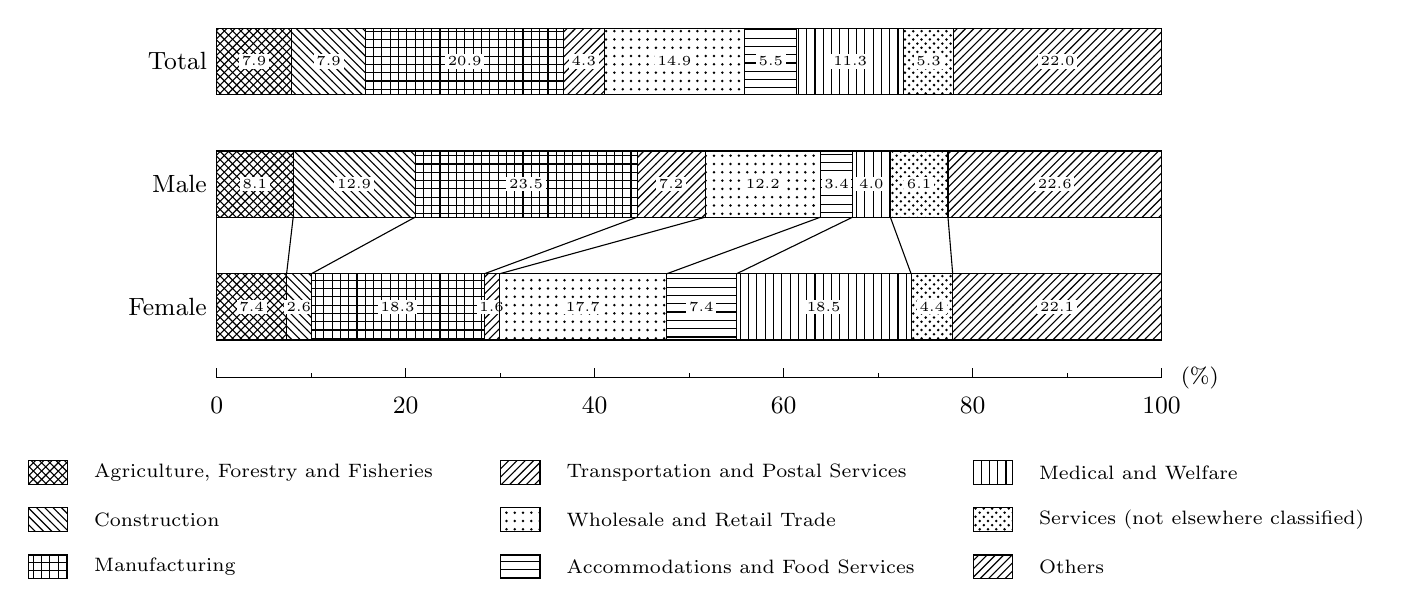
\begin{tikzpicture}[scale=1.20]
            \definecolor{color1}{RGB}{200,200,200} 
            \definecolor{color2}{RGB}{150,150,150} 
            \definecolor{color3}{RGB}{100,100,100}
            \definecolor{color4}{RGB}{250,200,200}
            \definecolor{color5}{RGB}{200,150,150}
            \definecolor{color6}{RGB}{150,100,100}
            \definecolor{color7}{RGB}{100,50,50}
            \definecolor{color8}{RGB}{50,0,0}
            \definecolor{color9}{RGB}{0,0,0}
            
            % Total bar
            \draw[fill=color1, pattern=crosshatch] (2,9) rectangle (2.79,9.7) node[pos=0.5, fill=white, inner sep=1pt] {\tiny 7.9};
            \draw[fill=color2, pattern=north west lines] (2.79,9) rectangle (3.58,9.7) node[pos=0.5, fill=white, inner sep=1pt] {\tiny 7.9};
            \draw[fill=color3, pattern=grid] (3.58,9) rectangle (5.67,9.7) node[pos=0.5, fill=white, inner sep=1pt] {\tiny 20.9};
            \draw[fill=color4, pattern=north east lines] (5.67,9) rectangle (6.10,9.7) node[pos=0.5, fill=white, inner sep=1pt] {\tiny 4.3}; 
            \draw[fill=color5, pattern=dots] (6.10,9) rectangle (7.59,9.7) node[pos=0.5, fill=white, inner sep=1pt] {\tiny 14.9}; 
            \draw[fill=color6, pattern=horizontal lines] (7.59,9) rectangle (8.14,9.7) node[pos=0.5, fill=white, inner sep=1pt] {\tiny 5.5};
            \draw[fill=color7, pattern=vertical lines] (8.14,9) rectangle (9.27,9.7) node[pos=0.5, fill=white, inner sep=1pt] {\tiny 11.3};
            \draw[fill=color8, pattern=crosshatch dots] (9.27,9) rectangle (9.80,9.7) node[pos=0.5, fill=white, inner sep=1pt] {\tiny 5.3};
            \draw[fill=color9, pattern=north east lines] (9.80,9) rectangle (12,9.7) node[pos=0.5, fill=white, inner sep=1pt] {\tiny 22.0}; 
            
            % Male bar
            \draw[fill=color1, pattern=crosshatch] (2,7.7) rectangle (2.81,8.4) node[pos=0.5, fill=white, inner sep=1pt] {\tiny 8.1};
            \draw[fill=color2, pattern=north west lines] (2.81,7.7) rectangle (4.10,8.4) node[pos=0.5, fill=white, inner sep=1pt] {\tiny 12.9};
            \draw[fill=color3, pattern=grid] (4.10,7.7) rectangle (6.45,8.4) node[pos=0.5, fill=white, inner sep=1pt] {\tiny 23.5};
            \draw[fill=color4, pattern=north east lines] (6.45,7.7) rectangle (7.17,8.4) node[pos=0.5, fill=white, inner sep=1pt] {\tiny 7.2}; 
            \draw[fill=color5, pattern=dots] (7.17,7.7) rectangle (8.39,8.4) node[pos=0.5, fill=white, inner sep=1pt] {\tiny 12.2}; 
            \draw[fill=color6, pattern=horizontal lines] (8.39,7.7) rectangle (8.73,8.4) node[pos=0.5, fill=white, inner sep=1pt] {\tiny 3.4};
            \draw[fill=color7, pattern=vertical lines] (8.73,7.7) rectangle (9.13,8.4) node[pos=0.5, fill=white, inner sep=1pt] {\tiny 4.0};
            \draw[fill=color8, pattern=crosshatch dots] (9.13,7.7) rectangle (9.74,8.4) node[pos=0.5, fill=white, inner sep=1pt] {\tiny 6.1};
            \draw[fill=color9, pattern=north east lines] (9.74,7.7) rectangle (12,8.4) node[pos=0.5, fill=white, inner sep=1pt] {\tiny 22.6};
            
            % Female bar
            \draw[fill=color1, pattern=crosshatch] (2,6.4) rectangle (2.74,7.1) node[pos=0.5, fill=white, inner sep=1pt] {\tiny 7.4};
            \draw[fill=color2, pattern=north west lines] (2.74,6.4) rectangle (3.00,7.1) node[pos=0.5, fill=white, inner sep=1pt] {\tiny 2.6};
            \draw[fill=color3, pattern=grid] (3.00,6.4) rectangle (4.83,7.1) node[pos=0.5, fill=white, inner sep=1pt] {\tiny 18.3};
            \draw[fill=color4, pattern=north east lines] (4.83,6.4) rectangle (4.99,7.1) node[pos=0.5, fill=white, inner sep=1pt] {\tiny 1.6}; 
            \draw[fill=color5, pattern=dots] (4.99,6.4) rectangle (6.76,7.1) node[pos=0.5, fill=white, inner sep=1pt] {\tiny 17.7}; 
            \draw[fill=color6, pattern=horizontal lines] (6.76,6.4) rectangle (7.50,7.1) node[pos=0.5, fill=white, inner sep=1pt] {\tiny 7.4};
            \draw[fill=color7, pattern=vertical lines] (7.50,6.4) rectangle (9.35,7.1) node[pos=0.5, fill=white, inner sep=1pt] {\tiny 18.5};
            \draw[fill=color8, pattern=crosshatch dots] (9.35,6.4) rectangle (9.79,7.1) node[pos=0.5, fill=white, inner sep=1pt] {\tiny 4.4};
            \draw[fill=color9, pattern=north east lines] (9.79,6.4) rectangle (12,7.1) node[pos=0.5, fill=white, inner sep=1pt] {\tiny 22.1}; 
            
            % Male to Female guidelines
            \draw[thin] (2,7.7) -- (2,7.1);
            \draw[thin] (2.81,7.7) -- (2.74,7.1);
            \draw[thin] (4.10,7.7) -- (3.00,7.1);
            \draw[thin] (6.45,7.7) -- (4.83,7.1);
            \draw[thin] (7.17,7.7) -- (4.99,7.1);
            \draw[thin] (8.39,7.7) -- (6.76,7.1);
            \draw[thin] (8.73,7.7) -- (7.50,7.1);
            \draw[thin] (9.13,7.7) -- (9.35,7.1);
            \draw[thin] (9.74,7.7) -- (9.79,7.1);
            \draw[thin] (12,7.7) -- (12,7.1);
            
            % Labels
            \node[anchor=east] at (2,9.35) {\small Total};
            \node[anchor=east] at (2,8.05) {\small Male};
            \node[anchor=east] at (2,6.75) {\small Female};
            
            % X-axis
            \draw (2,6) -- (12,6);
            \foreach \x in {0,20,40,60,80,100}
                \draw (2+\x/10,6) -- (2+\x/10,6.1) node[anchor=north] at (2+\x/10,5.9) {\small \x};
            \foreach \x in {10,30,50,70,90}
                \draw (2+\x/10,6) -- (2+\x/10,6.05);
            \node[anchor=west, font=\footnotesize] at (12.1,6) {(\%)};
            
            % Legend
            \node[anchor=west, fill=color1, pattern=crosshatch, minimum width=0.5cm, minimum height=0.3cm, draw] at (0,5) {};
            \node[anchor=west] at (0.6,5) {\scriptsize Agriculture, Forestry and Fisheries};
            \node[anchor=west, fill=color2, pattern=north west lines, minimum width=0.5cm, minimum height=0.3cm, draw] at (0,4.5) {};
            \node[anchor=west] at (0.6,4.5) {\scriptsize Construction};
            \node[anchor=west, fill=color3, pattern=grid, minimum width=0.5cm, minimum height=0.3cm, draw] at (0,4) {};
            \node[anchor=west] at (0.6,4) {\scriptsize Manufacturing};
            \node[anchor=west, fill=color4, pattern=north east lines, minimum width=0.5cm, minimum height=0.3cm, draw] at (5,5) {};
            \node[anchor=west] at (5.6,5) {\scriptsize Transportation and Postal Services};
            \node[anchor=west, fill=color5, pattern=dots, minimum width=0.5cm, minimum height=0.3cm, draw] at (5,4.5) {};
            \node[anchor=west] at (5.6,4.5) {\scriptsize Wholesale and Retail Trade};
            \node[anchor=west, fill=color6, pattern=horizontal lines, minimum width=0.5cm, minimum height=0.3cm, draw] at (5,4) {};
            \node[anchor=west] at (5.6,4) {\scriptsize Accommodations and Food Services};
            \node[anchor=west, fill=color7, pattern=vertical lines, minimum width=0.5cm, minimum height=0.3cm, draw] at (10,5) {};
            \node[anchor=west] at (10.6,5) {\scriptsize Medical and Welfare};
            \node[anchor=west, fill=color8, pattern=crosshatch dots, minimum width=0.5cm, minimum height=0.3cm, draw] at (10,4.5) {};
            \node[anchor=west] at (10.6,4.5) {\scriptsize Services (not elsewhere classified)};
            \node[anchor=west, fill=color9, pattern=north east lines, minimum width=0.5cm, minimum height=0.3cm, draw] at (10,4) {};
            \node[anchor=west] at (10.6,4) {\scriptsize Others};
        \end{tikzpicture}
        \caption{2010}
        \label{fig:fukushima_employment_2010}
    \end{subfigure}
    
    \vspace{1cm}
    
    \begin{subfigure}[b]{\textwidth}
        \centering
        % (b) 2015年のグラフ
        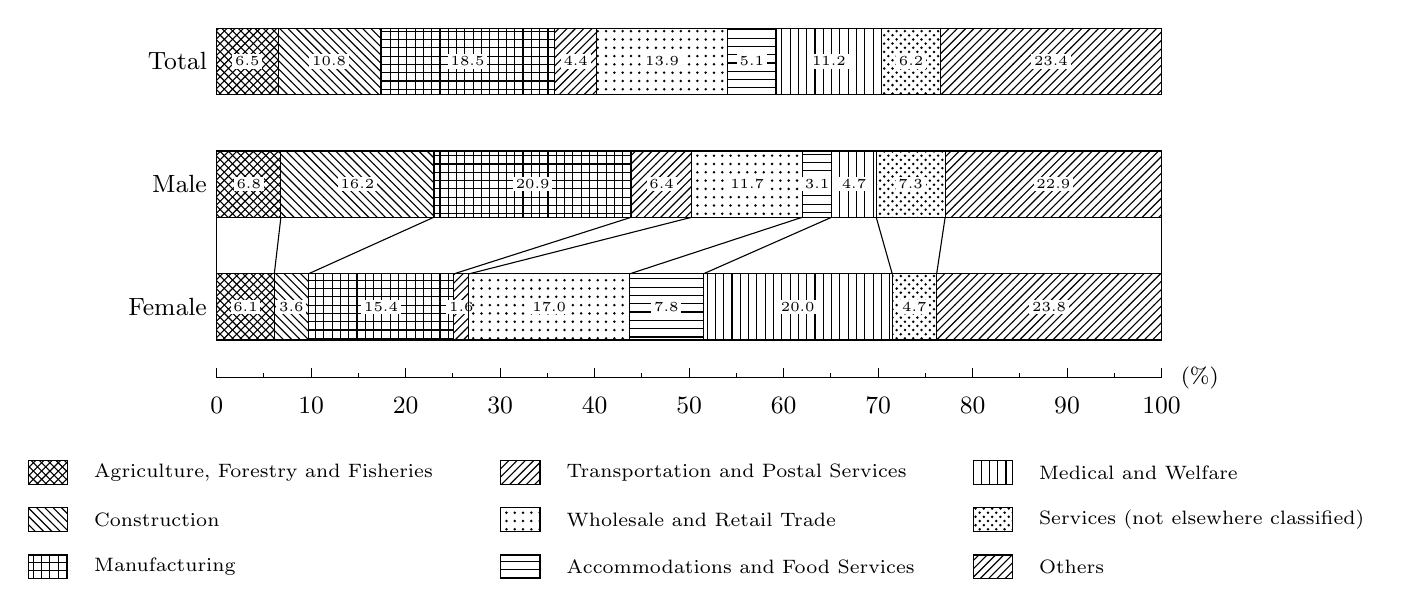
\begin{tikzpicture}[scale=1.20]
            \definecolor{color1}{RGB}{200,200,200} 
            \definecolor{color2}{RGB}{150,150,150} 
            \definecolor{color3}{RGB}{100,100,100}
            \definecolor{color4}{RGB}{250,200,200}
            \definecolor{color5}{RGB}{200,150,150}
            \definecolor{color6}{RGB}{150,100,100}
            \definecolor{color7}{RGB}{100,50,50}
            \definecolor{color8}{RGB}{50,0,0}
            \definecolor{color9}{RGB}{0,0,0}
            
            % Total bar
            \draw[fill=color1, pattern=crosshatch] (2.00,9) rectangle (2.65,9.7) node[pos=0.5, fill=white, inner sep=1pt] {\tiny 6.5};
            \draw[fill=color2, pattern=north west lines] (2.65,9) rectangle (3.73,9.7) node[pos=0.5, fill=white, inner sep=1pt] {\tiny 10.8};
            \draw[fill=color3, pattern=grid] (3.73,9) rectangle (5.58,9.7) node[pos=0.5, fill=white, inner sep=1pt] {\tiny 18.5};
            \draw[fill=color4, pattern=north east lines] (5.58,9) rectangle (6.02,9.7) node[pos=0.5, fill=white, inner sep=1pt] {\tiny 4.4}; 
            \draw[fill=color5, pattern=dots] (6.02,9) rectangle (7.41,9.7) node[pos=0.5, fill=white, inner sep=1pt] {\tiny 13.9}; 
            \draw[fill=color6, pattern=horizontal lines] (7.41,9) rectangle (7.92,9.7) node[pos=0.5, fill=white, inner sep=1pt] {\tiny 5.1};
            \draw[fill=color7, pattern=vertical lines] (7.92,9) rectangle (9.04,9.7) node[pos=0.5, fill=white, inner sep=1pt] {\tiny 11.2};
            \draw[fill=color8, pattern=crosshatch dots] (9.04,9) rectangle (9.66,9.7) node[pos=0.5, fill=white, inner sep=1pt] {\tiny 6.2};
            \draw[fill=color9, pattern=north east lines] (9.66,9) rectangle (12,9.7) node[pos=0.5, fill=white, inner sep=1pt] {\tiny 23.4}; 
            
            % Male bar
            \draw[fill=color1, pattern=crosshatch] (2.00,7.7) rectangle (2.68,8.4) node[pos=0.5, fill=white, inner sep=1pt] {\tiny 6.8};
            \draw[fill=color2, pattern=north west lines] (2.68,7.7) rectangle (4.30,8.4) node[pos=0.5, fill=white, inner sep=1pt] {\tiny 16.2};
            \draw[fill=color3, pattern=grid] (4.30,7.7) rectangle (6.39,8.4) node[pos=0.5, fill=white, inner sep=1pt] {\tiny 20.9};
            \draw[fill=color4, pattern=north east lines] (6.39,7.7) rectangle (7.03,8.4) node[pos=0.5, fill=white, inner sep=1pt] {\tiny 6.4}; 
            \draw[fill=color5, pattern=dots] (7.03,7.7) rectangle (8.20,8.4) node[pos=0.5, fill=white, inner sep=1pt] {\tiny 11.7}; 
            \draw[fill=color6, pattern=horizontal lines] (8.20,7.7) rectangle (8.51,8.4) node[pos=0.5, fill=white, inner sep=1pt] {\tiny 3.1};
            \draw[fill=color7, pattern=vertical lines] (8.51,7.7) rectangle (8.98,8.4) node[pos=0.5, fill=white, inner sep=1pt] {\tiny 4.7};
            \draw[fill=color8, pattern=crosshatch dots] (8.98,7.7) rectangle (9.71,8.4) node[pos=0.5, fill=white, inner sep=1pt] {\tiny 7.3};
            \draw[fill=color9, pattern=north east lines] (9.71,7.7) rectangle (12,8.4) node[pos=0.5, fill=white, inner sep=1pt] {\tiny 22.9};
            
            % Female bar
            \draw[fill=color1, pattern=crosshatch] (2.00,6.4) rectangle (2.61,7.1) node[pos=0.5, fill=white, inner sep=1pt] {\tiny 6.1};
            \draw[fill=color2, pattern=north west lines] (2.61,6.4) rectangle (2.97,7.1) node[pos=0.5, fill=white, inner sep=1pt] {\tiny 3.6};
            \draw[fill=color3, pattern=grid] (2.97,6.4) rectangle (4.51,7.1) node[pos=0.5, fill=white, inner sep=1pt] {\tiny 15.4};
            \draw[fill=color4, pattern=north east lines] (4.51,6.4) rectangle (4.67,7.1) node[pos=0.5, fill=white, inner sep=1pt] {\tiny 1.6}; 
            \draw[fill=color5, pattern=dots] (4.67,6.4) rectangle (6.37,7.1) node[pos=0.5, fill=white, inner sep=1pt] {\tiny 17.0}; 
            \draw[fill=color6, pattern=horizontal lines] (6.37,6.4) rectangle (7.15,7.1) node[pos=0.5, fill=white, inner sep=1pt] {\tiny 7.8};
            \draw[fill=color7, pattern=vertical lines] (7.15,6.4) rectangle (9.15,7.1) node[pos=0.5, fill=white, inner sep=1pt] {\tiny 20.0};
            \draw[fill=color8, pattern=crosshatch dots] (9.15,6.4) rectangle (9.62,7.1) node[pos=0.5, fill=white, inner sep=1pt] {\tiny 4.7};
            \draw[fill=color9, pattern=north east lines] (9.62,6.4) rectangle (12,7.1) node[pos=0.5, fill=white, inner sep=1pt] {\tiny 23.8}; 
            
            % Male to Female guidelines
            \draw[thin] (2.00,7.7) -- (2.00,7.1);
            \draw[thin] (12,7.7) -- (12,7.1);
            
            \draw[thin] (2.68,7.7) -- (2.61,7.1);      % Agriculture, Forestry and Fisheries
            \draw[thin] (4.30,7.7) -- (2.97,7.1);      % Construction
            \draw[thin] (6.39,7.7) -- (4.51,7.1);      % Manufacturing
            \draw[thin] (7.03,7.7) -- (4.67,7.1);      % Transportation and Postal Services
            \draw[thin] (8.20,7.7) -- (6.37,7.1);      % Wholesale and Retail Trade
            \draw[thin] (8.51,7.7) -- (7.15,7.1);      % Accommodations and Food Services
            \draw[thin] (8.98,7.7) -- (9.15,7.1);      % Medical and Welfare
            \draw[thin] (9.71,7.7) -- (9.62,7.1);      % Services (not elsewhere classified)
            
            % Labels
            \node[anchor=east] at (2,9.35) {\small Total};
            \node[anchor=east] at (2,8.05) {\small Male};
            \node[anchor=east] at (2,6.75) {\small Female};
            
            % X-axis
            \draw (2,6) -- (12,6);
            \foreach \x in {0,10,20,30,40,50,60,70,80,90,100}
                \draw (2+\x/10,6) -- (2+\x/10,6.1) node[anchor=north] at (2+\x/10,5.9) {\small \x};
            \foreach \x in {5,15,25,35,45,55,65,75,85,95}
                \draw (2+\x/10,6) -- (2+\x/10,6.05);
            \node[anchor=west, font=\footnotesize] at (12.1,6) {(\%)};
            
            % Legend
            \node[anchor=west, fill=color1, pattern=crosshatch, minimum width=0.5cm, minimum height=0.3cm, draw] at (0,5) {};
            \node[anchor=west] at (0.6,5) {\scriptsize Agriculture, Forestry and Fisheries};
            \node[anchor=west, fill=color2, pattern=north west lines, minimum width=0.5cm, minimum height=0.3cm, draw] at (0,4.5) {};
            \node[anchor=west] at (0.6,4.5) {\scriptsize Construction};
            \node[anchor=west, fill=color3, pattern=grid, minimum width=0.5cm, minimum height=0.3cm, draw] at (0,4) {};
            \node[anchor=west] at (0.6,4) {\scriptsize Manufacturing};
            \node[anchor=west, fill=color4, pattern=north east lines, minimum width=0.5cm, minimum height=0.3cm, draw] at (5,5) {};
            \node[anchor=west] at (5.6,5) {\scriptsize Transportation and Postal Services};
            \node[anchor=west, fill=color5, pattern=dots, minimum width=0.5cm, minimum height=0.3cm, draw] at (5,4.5) {};
            \node[anchor=west] at (5.6,4.5) {\scriptsize Wholesale and Retail Trade};
            \node[anchor=west, fill=color6, pattern=horizontal lines, minimum width=0.5cm, minimum height=0.3cm, draw] at (5,4) {};
            \node[anchor=west] at (5.6,4) {\scriptsize Accommodations and Food Services};
            \node[anchor=west, fill=color7, pattern=vertical lines, minimum width=0.5cm, minimum height=0.3cm, draw] at (10,5) {};
            \node[anchor=west] at (10.6,5) {\scriptsize Medical and Welfare};
            \node[anchor=west, fill=color8, pattern=crosshatch dots, minimum width=0.5cm, minimum height=0.3cm, draw] at (10,4.5) {};
            \node[anchor=west] at (10.6,4.5) {\scriptsize Services (not elsewhere classified)};
            \node[anchor=west, fill=color9, pattern=north east lines, minimum width=0.5cm, minimum height=0.3cm, draw] at (10,4) {};
            \node[anchor=west] at (10.6,4) {\scriptsize Others};
        \end{tikzpicture}
        \caption{2015}
        \label{fig:fukushima_employment_2015}
    \end{subfigure}
    
    % Combined Note and Source
    \vspace{0.5cm}
    \begin{minipage}{\textwidth}
        \footnotesize
        \textit{Note}: "Others" includes "Mining and Quarrying of Stone and Gravel", "Electricity, Gas, Heat Supply and Water", "Information and Communications", "Finance and Insurance", "Real Estate and Goods Rental and Leasing", "Scientific Research, Professional and Technical Services", "Living-Related and Personal Services and Amusement Services", "Education, Learning Support", "Compound Services", "Government (except elsewhere classified)" and "Industries Unable to Classify".
        
        \vspace{0.1cm}
        
        \textit{Source}: Statistics Bureau, Ministry of Internal Affairs and Communications, Japan. "2010 and 2015 Population Census."
    \end{minipage}
    
    \caption{Proportion of Employed Persons Aged 15 and Over by Industry and Gender - Fukushima (2010 and 2015)} 
    \label{fig:fukushima_employment_combined}
\end{figure}

%%%%%%%%%%%%%%%%%%%%%%%%%%%%%%%%%%%%%%%%%%%%%%

%福島県の職業(Occupation)別の男女別15歳以上就業者について、従業上の地位別(Employment type)の割合をみると、全職業(Total)では、男性の場合、「正規の職員・従業員」の割合は「事務従事者」が62.7%だが女性では40.1%である。一方、「パート・アルバイト・その他」の割合は、女性が36.8%に対して男性は9.8%である。自然災害が非正規労働者により大きな負の影響を及ぼすことが知られており、このような雇用形態のジェンダー格差は、そのまま自然災害影響のジェンダーギャップとして現れる。特筆すべきは、農林水産業では73.0%の男性が「Self-employed」と回答しているのに対し、女性の方は81.2%が「Family worker」と回答していることである。つまりFamily businessにおいては夫がオーナーであり、妻はその従業員であるという性別役割分担の存在が見てとれる。これは自然災害時に、夫よりも妻の労働の増減が危機に対する調整弁の役割を果たすことを意味する。

\begin{figure}[!t]
\begin{adjustbox}{width=\textwidth}
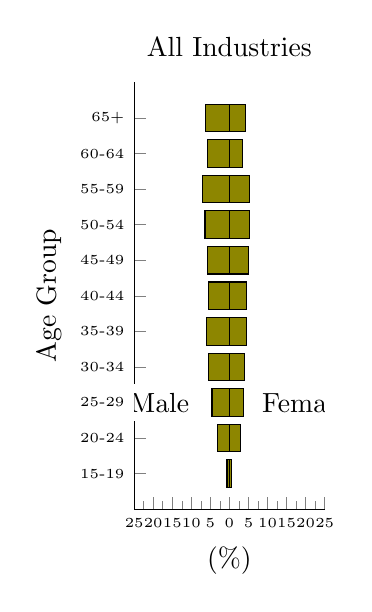
\begin{tikzpicture}
\begin{axis}[
    width=0.33\textwidth,
    height=7cm,
    xbar stacked,
    xmin=-25,
    xmax=25,
    xtick={-25, -20, -15, -10, -5, 0, 5, 10, 15, 20, 25},
    xticklabels={25, 20, 15, 10, 5, 0, 5, 10, 15, 20, 25},
    xlabel={(\%)},
    ylabel={Age Group},
    ytick={1,2,3,4,5,6,7,8,9,10,11},
    yticklabels={15-19, 20-24, 25-29, 30-34, 35-39, 40-44, 45-49, 50-54, 55-59, 60-64, 65+},
    title={All Industries},
    axis y line*=left,
    axis x line*=bottom,
    bar width=3.5mm,
    xticklabel style={font=\tiny},
    yticklabel style={font=\tiny},
    xlabel style={font=\normalsize},
    minor x tick num=1,
    grid style={line width=.1pt, draw=gray!20},
    major grid style={line width=.2pt,draw=gray!50},
]
\addplot[xbar, fill=olive] coordinates {(-6.2968,11) (-5.7348,10) (-7.0630,9) (-6.4160,8) (-5.8457,7) (-5.4109,6) (-6.0469,5) (-5.5079,4) (-4.5710,3) (-3.1366,2) (-0.6502,1)};
\addplot[xbar, fill=olive] coordinates {(4.1861,11) (3.5393,10) (5.1758,9) (5.2826,8) (4.9579,7) (4.4568,6) (4.5115,5) (4.0165,4) (3.6677,3) (2.9304,2) (0.5957,1)};
\node[anchor=east, fill=white] at (axis cs:-8,3) {Male};
\node[anchor=west, fill=white] at (axis cs:6,3) {Female};
\end{axis}
\end{tikzpicture}
\hfill
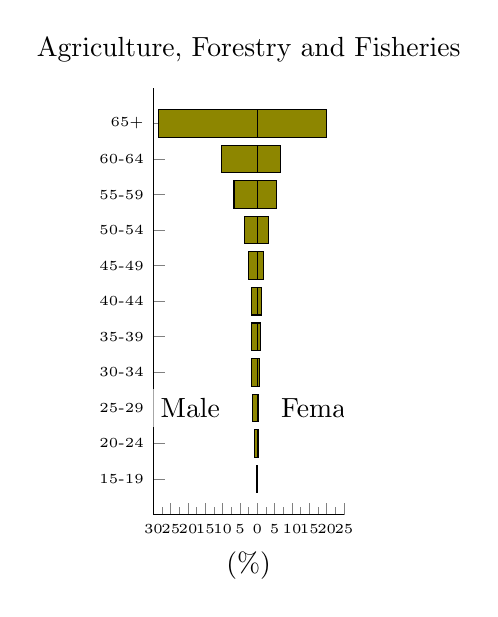
\begin{tikzpicture}
\begin{axis}[
    width=0.33\textwidth,
    height=7cm,
    xbar stacked,
    xmin=-30,
    xmax=25,
    xtick={-30, -25, -20, -15, -10, -5, 0, 5, 10, 15, 20, 25},
    xticklabels={30, 25, 20, 15, 10, 5, 0, 5, 10, 15, 20, 25},
    xlabel={(\%)},
    ytick={1,2,3,4,5,6,7,8,9,10,11},
    yticklabels={15-19, 20-24, 25-29, 30-34, 35-39, 40-44, 45-49, 50-54, 55-59, 60-64, 65+},
    yticklabel pos=right,
    title={Agriculture, Forestry and Fisheries},
    axis y line*=left,
    axis x line*=bottom,
    bar width=3.5mm,
    xticklabel style={font=\tiny},
    yticklabel style={font=\tiny},
    xlabel style={font=\normalsize},
    minor x tick num=1,
    grid style={line width=.1pt, draw=gray!20},
    major grid style={line width=.2pt,draw=gray!50},
]
\addplot[xbar, fill=olive] coordinates {(-28.5896,11) (-10.3951,10) (-6.7607,9) (-3.8248,8) (-2.5634,7) (-1.6352,6) (-1.6058,5) (-1.6520,4) (-1.2908,3) (-0.8218,2) (-0.1694,1)};
\addplot[xbar, fill=olive] coordinates {(20.0734,11) (6.5899,10) (5.5664,9) (3.2718,8) (1.7640,7) (1.1144,6) (0.8792,5) (0.6888,4) (0.4494,3) (0.2394,2) (0.0546,1)};
\node[anchor=east, fill=white] at (axis cs:-8,3) {Male};
\node[anchor=west, fill=white] at (axis cs:4,3) {Female};
\end{axis}
\end{tikzpicture}
\hfill
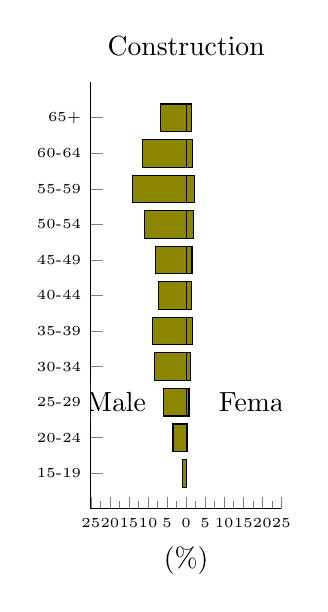
\begin{tikzpicture}
\begin{axis}[
    width=0.33\textwidth,
    height=7cm,
    xbar stacked,
    xmin=-25,
    xmax=25,
    xtick={-25, -20, -15, -10, -5, 0, 5, 10, 15, 20, 25},
    xticklabels={25, 20, 15, 10, 5, 0, 5, 10, 15, 20, 25},
    xlabel={(\%)},
    ytick={1,2,3,4,5,6,7,8,9,10,11},
    yticklabels={15-19, 20-24, 25-29, 30-34, 35-39, 40-44, 45-49, 50-54, 55-59, 60-64, 65+},
    yticklabel pos=right,
    title={Construction},
    axis y line*=left,
    axis x line*=bottom,
    bar width=3.5mm,
    xticklabel style={font=\tiny},
    yticklabel style={font=\tiny},
    xlabel style={font=\normalsize},
    minor x tick num=1,
    grid style={line width=.1pt, draw=gray!20},
    major grid style={line width=.2pt,draw=gray!50},
]
\addplot[xbar, fill=olive] coordinates {(-6.6875,11) (-11.4525,10) (-14.1118,9) (-10.9621,8) (-8.1361,7) (-7.1541,6) (-8.9182,5) (-8.3385,4) (-6.0411,3) (-3.4449,2) (-0.8749,1)};
\addplot[xbar, fill=olive] coordinates {(1.2939,11) (1.7058,10) (2.1069,9) (1.8165,8) (1.5332,7) (1.4439,6) (1.6165,5) (1.2035,4) (0.7380,3) (0.3726,2) (0.0476,1)};
\node[anchor=east, fill=white] at (axis cs:-8,3) {Male};
\node[anchor=west, fill=white] at (axis cs:6,3) {Female};
\end{axis}
\end{tikzpicture}
\end{adjustbox}

% 2行目のグラフ
\begin{adjustbox}{width=\textwidth}
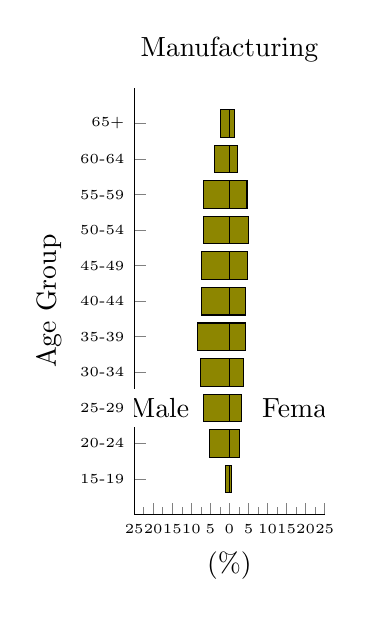
\begin{tikzpicture}
\begin{axis}[
    width=0.33\textwidth,
    height=7cm,
    xbar stacked,
    xmin=-25,
    xmax=25,
    xtick={-25, -20, -15, -10, -5, 0, 5, 10, 15, 20, 25},
    xticklabels={25, 20, 15, 10, 5, 0, 5, 10, 15, 20, 25},
    xlabel={(\%)},
    ylabel={Age Group},
    ytick={1,2,3,4,5,6,7,8,9,10,11},
    yticklabels={15-19, 20-24, 25-29, 30-34, 35-39, 40-44, 45-49, 50-54, 55-59, 60-64, 65+},
    title={Manufacturing},
    axis y line*=left,
    axis x line*=bottom,
    bar width=3.5mm,
    xticklabel style={font=\tiny},
    yticklabel style={font=\tiny},
    xlabel style={font=\normalsize},
    minor x tick num=1,
    grid style={line width=.1pt, draw=gray!20},
    major grid style={line width=.2pt,draw=gray!50},
]
\addplot[xbar, fill=olive] coordinates {(-2.4548,11) (-3.9043,10) (-6.7497,9) (-6.7481,8) (-7.4452,7) (-7.3451,6) (-8.3323,5) (-7.6527,4) (-6.7811,3) (-5.1740,2) (-0.9664,1)};
\addplot[xbar, fill=olive] coordinates {(1.2771,11) (2.1461,10) (4.6067,9) (4.9622,8) (4.8095,7) (4.2896,6) (4.3236,5) (3.6345,4) (3.1567,3) (2.7400,2) (0.5002,1)};
\node[anchor=east, fill=white] at (axis cs:-8,3) {Male};
\node[anchor=west, fill=white] at (axis cs:6,3) {Female};
\end{axis}
\end{tikzpicture}
\hfill
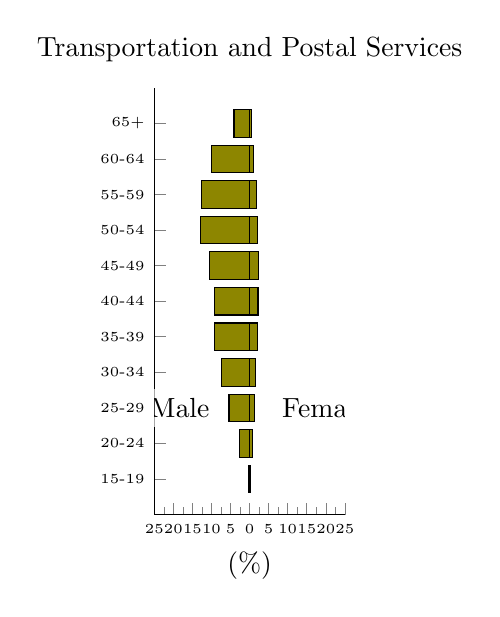
\begin{tikzpicture}
\begin{axis}[
    width=0.33\textwidth,
    height=7cm,
    xbar stacked,
    xmin=-25,
    xmax=25,
    xtick={-25, -20, -15, -10, -5, 0, 5, 10, 15, 20, 25},
    xticklabels={25, 20, 15, 10, 5, 0, 5, 10, 15, 20, 25},
    xlabel={(\%)},
    ytick={1,2,3,4,5,6,7,8,9,10,11},
    yticklabels={15-19, 20-24, 25-29, 30-34, 35-39, 40-44, 45-49, 50-54, 55-59, 60-64, 65+},
    yticklabel pos=right,
    title={Transportation and Postal Services},
    axis y line*=left,
    axis x line*=bottom,
    bar width=3.5mm,
    xticklabel style={font=\tiny},
    yticklabel style={font=\tiny},
    xlabel style={font=\normalsize},
    minor x tick num=1,
    grid style={line width=.1pt, draw=gray!20},
    major grid style={line width=.2pt,draw=gray!50},
]
\addplot[xbar, fill=olive] coordinates {(-4.0825,11) (-10.0013,10) (-12.6223,9) (-12.8891,8) (-10.6053,7) (-9.1725,6) (-9.1152,5) (-7.3627,4) (-5.4052,3) (-2.7445,2) (-0.3836,1)};
\addplot[xbar, fill=olive] coordinates {(0.5070,11) (1.0691,10) (1.8274,9) (2.1030,8) (2.3609,7) (2.2154,6) (2.0787,5) (1.4373,4) (1.1948,3) (0.7164,2) (0.1058,1)};
\node[anchor=east, fill=white] at (axis cs:-8,3) {Male};
\node[anchor=west, fill=white] at (axis cs:6,3) {Female};
\end{axis}
\end{tikzpicture}
\hfill
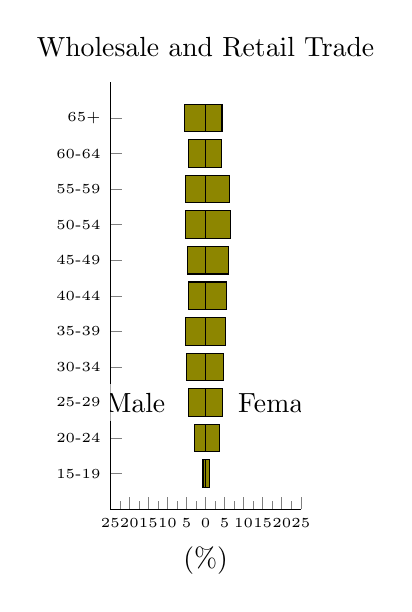
\begin{tikzpicture}
\begin{axis}[
    width=0.33\textwidth,
    height=7cm,
    xbar stacked,
    xmin=-25,
    xmax=25,
    xtick={-25, -20, -15, -10, -5, 0, 5, 10, 15, 20, 25},
    xticklabels={25, 20, 15, 10, 5, 0, 5, 10, 15, 20, 25},
    xlabel={(\%)},
    ytick={1,2,3,4,5,6,7,8,9,10,11},
    yticklabels={15-19, 20-24, 25-29, 30-34, 35-39, 40-44, 45-49, 50-54, 55-59, 60-64, 65+},
    yticklabel pos=right,
    title={Wholesale and Retail Trade},
    axis y line*=left,
    axis x line*=bottom,
    bar width=3.5mm,
    xticklabel style={font=\tiny},
    yticklabel style={font=\tiny},
    xlabel style={font=\normalsize},
    minor x tick num=1,
    grid style={line width=.1pt, draw=gray!20},
    major grid style={line width=.2pt,draw=gray!50},
]
\addplot[xbar, fill=olive] coordinates {(-5.6034,11) (-4.4603,10) (-5.3643,9) (-5.1647,8) (-4.7515,7) (-4.5047,6) (-5.3544,5) (-5.1161,4) (-4.4201,3) (-2.9335,2) (-0.6798,1)};
\addplot[xbar, fill=olive] coordinates {(4.3157,11) (4.1070,10) (6.2549,9) (6.4510,8) (6.0631,7) (5.4397,6) (5.2987,5) (4.7508,4) (4.3911,3) (3.5696,2) (1.0056,1)};
\node[anchor=east, fill=white] at (axis cs:-8,3) {Male};
\node[anchor=west, fill=white] at (axis cs:6,3) {Female};
\end{axis}
\end{tikzpicture}
\end{adjustbox}

% 3行目のグラフ
\begin{adjustbox}{width=\textwidth}
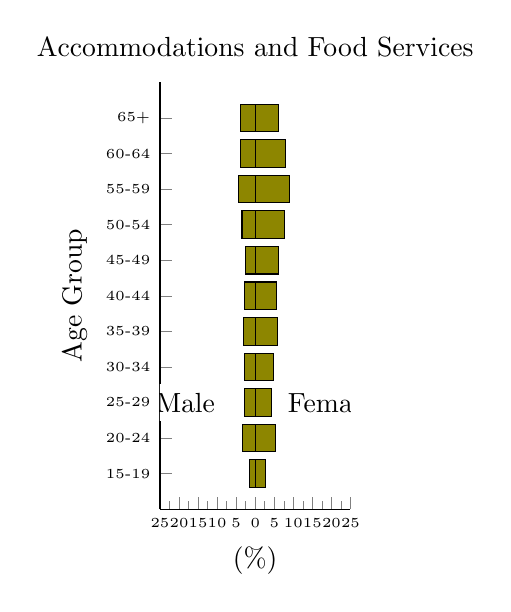
\begin{tikzpicture}
\begin{axis}[
    width=0.33\textwidth,
    height=7cm,
    xbar stacked,
    xmin=-25,
    xmax=25,
    xtick={-25, -20, -15, -10, -5, 0, 5, 10, 15, 20, 25},
    xticklabels={25, 20, 15, 10, 5, 0, 5, 10, 15, 20, 25},
 xlabel={(\%)},
    ylabel={Age Group},
    ytick={1,2,3,4,5,6,7,8,9,10,11},
    yticklabels={15-19, 20-24, 25-29, 30-34, 35-39, 40-44, 45-49, 50-54, 55-59, 60-64, 65+},
    title={Accommodations and Food Services},
    axis y line*=left,
    axis x line*=bottom,
    bar width=3.5mm,
    xticklabel style={font=\tiny},
    yticklabel style={font=\tiny},
    xlabel style={font=\normalsize},
    minor x tick num=1,
    grid style={line width=.1pt, draw=gray!20},
    major grid style={line width=.2pt,draw=gray!50},
]
\addplot[xbar, fill=olive] coordinates {(-3.8505,11) (-3.9093,10) (-4.2855,9) (-3.4547,8) (-2.6611,7) (-2.7884,6) (-3.0647,5) (-2.9217,4) (-2.9119,3) (-3.4410,2) (-1.4697,1)};
\addplot[xbar, fill=olive] coordinates {(6.1236,11) (7.9950,10) (9.0473,9) (7.6775,8) (6.0158,7) (5.6004,6) (5.7866,5) (4.7206,4) (4.3287,3) (5.2163,2) (2.7297,1)};
\node[anchor=east, fill=white] at (axis cs:-8,3) {Male};
\node[anchor=west, fill=white] at (axis cs:6,3) {Female};
\end{axis}
\end{tikzpicture}
\hfill
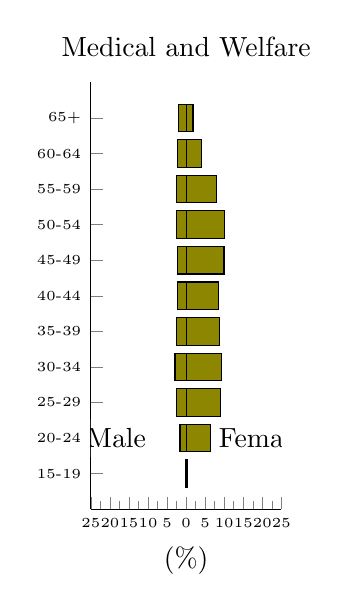
\begin{tikzpicture}
\begin{axis}[
    width=0.33\textwidth,
    height=7cm,
    xbar stacked,
    xmin=-25,
    xmax=25,
    xtick={-25, -20, -15, -10, -5, 0, 5, 10, 15, 20, 25},
    xticklabels={25, 20, 15, 10, 5, 0, 5, 10, 15, 20, 25},
    xlabel={(\%)},
    ytick={1,2,3,4,5,6,7,8,9,10,11},
    yticklabels={15-19, 20-24, 25-29, 30-34, 35-39, 40-44, 45-49, 50-54, 55-59, 60-64, 65+},
    yticklabel pos=right,
    title={Medical and Welfare},
    axis y line*=left,
    axis x line*=bottom,
    bar width=3.5mm,
    xticklabel style={font=\tiny},
    yticklabel style={font=\tiny},
    xlabel style={font=\normalsize},
    minor x tick num=1,
    grid style={line width=.1pt, draw=gray!20},
    major grid style={line width=.2pt,draw=gray!50},
]
\addplot[xbar, fill=olive] coordinates {(-2.0760,11) (-2.1576,10) (-2.4203,9) (-2.4234,8) (-2.3000,7) (-2.1796,6) (-2.5302,5) (-2.9330,4) (-2.5197,3) (-1.6072,2) (-0.1350,1)};
\addplot[xbar, fill=olive] coordinates {(1.8123,11) (4.0820,10) (8.0687,9) (10.0736,8) (9.9229,7) (8.4778,6) (8.8545,5) (9.3578,4) (9.1318,3) (6.4750,2) (0.4615,1)};
\node[anchor=east, fill=white] at (axis cs:-8,2) {Male};
\node[anchor=west, fill=white] at (axis cs:6,2) {Female};
\end{axis}
\end{tikzpicture}
\hfill
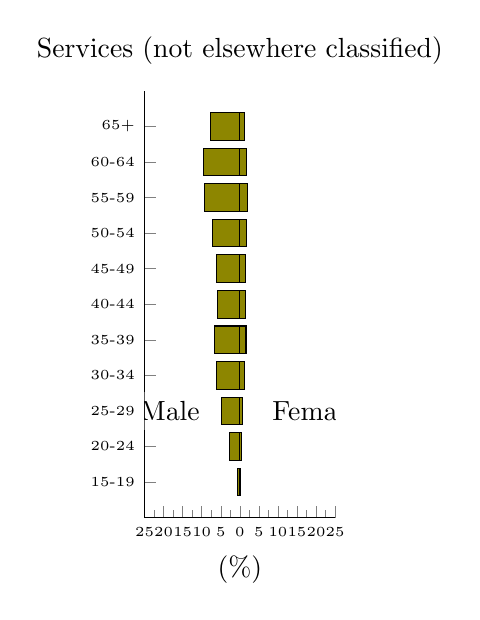
\begin{tikzpicture}
\begin{axis}[
    width=0.33\textwidth,
    height=7cm,
    xbar stacked,
    xmin=-25,
    xmax=25,
    xtick={-25, -20, -15, -10, -5, 0, 5, 10, 15, 20, 25},
    xticklabels={25, 20, 15, 10, 5, 0, 5, 10, 15, 20, 25},
    xlabel={(\%)},
    ytick={1,2,3,4,5,6,7,8,9,10,11},
    yticklabels={15-19, 20-24, 25-29, 30-34, 35-39, 40-44, 45-49, 50-54, 55-59, 60-64, 65+},
    yticklabel pos=right,
    title={Services (not elsewhere classified)},
    axis y line*=left,
    axis x line*=bottom,
    bar width=3.5mm,
    xticklabel style={font=\tiny},
    yticklabel style={font=\tiny},
    xlabel style={font=\normalsize},
    minor x tick num=1,
    grid style={line width=.1pt, draw=gray!20},
    major grid style={line width=.2pt,draw=gray!50},
]
\addplot[xbar, fill=olive] coordinates {(-7.5892,11) (-9.4724,10) (-9.3730,9) (-7.1919,8) (-6.1034,7) (-5.9352,6) (-6.6690,5) (-6.1825,4) (-4.8061,3) (-2.8135,2) (-0.5534,1)};
\addplot[xbar, fill=olive] coordinates {(1.2939,11) (1.7058,10) (2.1069,9) (1.8165,8) (1.5332,7) (1.4439,6) (1.6165,5) (1.2035,4) (0.7380,3) (0.3726,2) (0.0476,1)};
\node[anchor=east, fill=white] at (axis cs:-8,3) {Male};
\node[anchor=west, fill=white] at (axis cs:6,3) {Female};
\end{axis}
\end{tikzpicture}
\end{adjustbox}

\begin{flushleft}
\footnotesize
Source: Statistics Bureau, Ministry of Internal Affairs and Communications, Japan. "2010 Population Census."
\end{flushleft}


\caption{Proportion of Employed Persons Aged 15 and Over by Industry, Age (5-year groups), and Gender - Fukushima (2010)}
\label{fig:fukushima_Proportion_Employed}
\end{figure}

%%%%%%%%%%%%%%%%%%%%%%%%%%%%%%%%%%%%%%%%%%%%
%Labor force participation rate
%%%%%%%%%%%%%%%%%%%%%%%%%%%%%%%%%%%%%%%%%%%%
\begin{figure}[h!]

\begin{subfigure}{\textwidth}
\caption{Fukushima}
\begin{minipage}{0.48\textwidth}
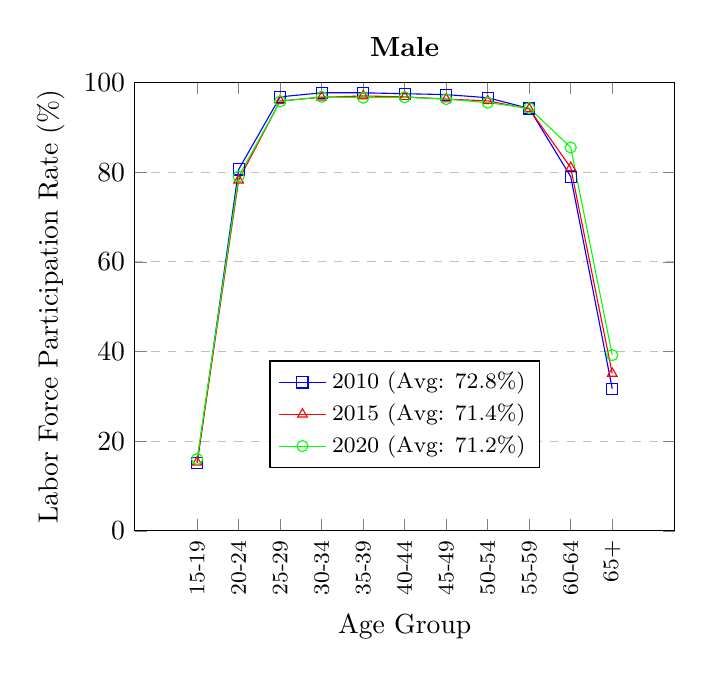
\begin{tikzpicture}
\begin{axis}[
    title={\textbf{Male}},
    xlabel={Age Group},
    ylabel={Labor Force Participation Rate (\%)},
    xmin=0, xmax=12,
    ymin=0, ymax=100,
    xtick={1,2,3,4,5,6,7,8,9,10,11},
    xticklabels={15-19,20-24,25-29,30-34,35-39,40-44,45-49,50-54,55-59,60-64,65+},
    x tick label style={rotate=90,anchor=east,font=\footnotesize},
    legend style={at={(0.5,0.38)},anchor=north,font=\footnotesize,
                  cells={anchor=west},
                  legend columns=1,
                  draw=black,fill=white,align=left},
    ymajorgrids=true,
    grid style=dashed,
    enlarge x limits={abs=0.5},
]

\addplot[color=blue,mark=square,] coordinates {
    (1,15.1)(2,80.6)(3,96.8)(4,97.7)(5,97.7)(6,97.5)(7,97.3)(8,96.6)(9,94.2)(10,79.0)(11,31.7)
};

\addplot[color=red,mark=triangle,] coordinates {
    (1,15.3)(2,78.2)(3,95.9)(4,96.7)(5,97.0)(6,96.8)(7,96.3)(8,95.9)(9,94.1)(10,81.0)(11,35.1)
};

\addplot[color=green,mark=o,] coordinates {
    (1,16.0)(2,79.0)(3,95.8)(4,96.8)(5,96.6)(6,96.7)(7,96.3)(8,95.5)(9,94.3)(10,85.5)(11,39.2)
};

\legend{
    2010 (Avg: 72.8\%),
    2015 (Avg: 71.4\%),
    2020 (Avg: 71.2\%)
}
\end{axis}
\end{tikzpicture}
\end{minipage}
\hfill
\begin{minipage}{0.48\textwidth}
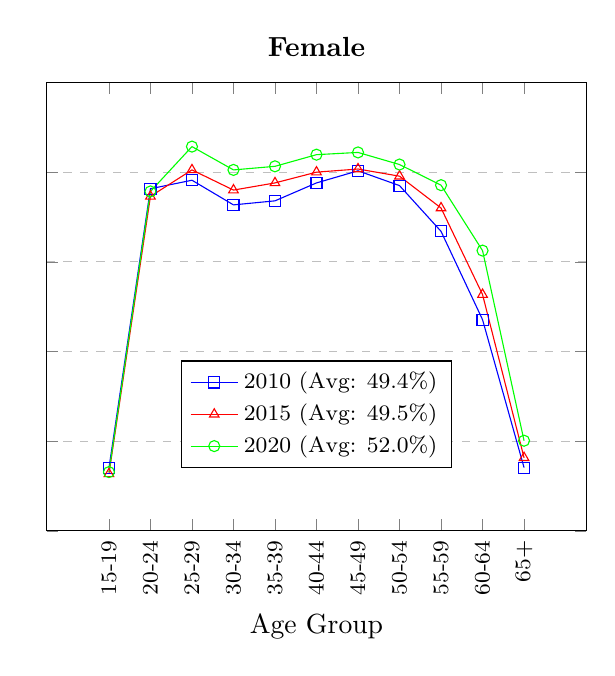
\begin{tikzpicture}
\begin{axis}[
    title={\textbf{Female}},
    xlabel={Age Group},
    ylabel={},
    xmin=0, xmax=12,
    ymin=0, ymax=100,
    xtick={1,2,3,4,5,6,7,8,9,10,11},
    xticklabels={15-19,20-24,25-29,30-34,35-39,40-44,45-49,50-54,55-59,60-64,65+},
    x tick label style={rotate=90,anchor=east,font=\footnotesize},
    legend style={at={(0.5,0.38)},anchor=north,font=\footnotesize,
                  cells={anchor=west},
                  legend columns=1,
                  draw=black,fill=white,align=left},
    ymajorgrids=true,
    grid style=dashed,
    yticklabels={,,},
    enlarge x limits={abs=0.5},
]

\addplot[color=blue,mark=square,] coordinates {
    (1,14.0)(2,76.3)(3,78.2)(4,72.7)(5,73.6)(6,77.6)(7,80.3)(8,77.0)(9,66.8)(10,47.1)(11,14.1)
};

\addplot[color=red,mark=triangle,] coordinates {
    (1,12.7)(2,74.6)(3,80.5)(4,76.0)(5,77.6)(6,80.0)(7,80.7)(8,79.1)(9,72.0)(10,52.7)(11,16.3)
};

\addplot[color=green,mark=o,] coordinates {
    (1,13.1)(2,75.7)(3,85.7)(4,80.5)(5,81.3)(6,83.9)(7,84.4)(8,81.7)(9,77.1)(10,62.5)(11,20.1)
};

\legend{
    2010 (Avg: 49.4\%),
    2015 (Avg: 49.5\%),
    2020 (Avg: 52.0\%)
}
\end{axis}
\end{tikzpicture}
\end{minipage}
\end{subfigure}

\vspace{0.5cm}

\begin{subfigure}{\textwidth}
\caption{Nationwide}
\begin{minipage}{0.48\textwidth}
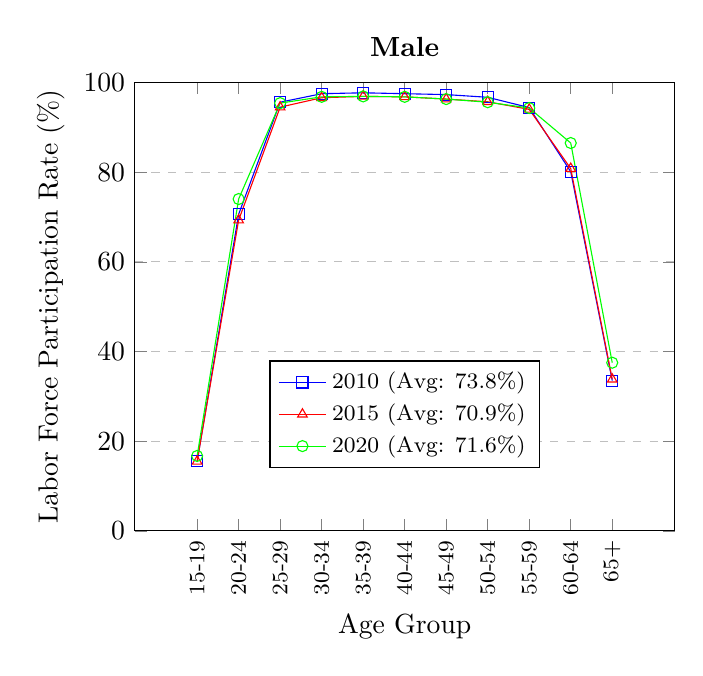
\begin{tikzpicture}
\begin{axis}[
    title={\textbf{Male}},
    xlabel={Age Group},
    ylabel={Labor Force Participation Rate (\%)},
    xmin=0, xmax=12,
    ymin=0, ymax=100,
    xtick={1,2,3,4,5,6,7,8,9,10,11},
    xticklabels={15-19,20-24,25-29,30-34,35-39,40-44,45-49,50-54,55-59,60-64,65+},
    x tick label style={rotate=90,anchor=east,font=\footnotesize},
    legend style={at={(0.5,0.38)},anchor=north,font=\footnotesize,
                  cells={anchor=west},
                  legend columns=1,
                  draw=black,fill=white,align=left},
    ymajorgrids=true,
    grid style=dashed,
    enlarge x limits={abs=0.5},
]

\addplot[color=blue,mark=square,] coordinates {
    (1,15.5)(2,70.6)(3,95.6)(4,97.5)(5,97.7)(6,97.5)(7,97.3)(8,96.7)(9,94.4)(10,80.1)(11,33.5)
};

\addplot[color=red,mark=triangle,] coordinates {
    (1,15.5)(2,69.3)(3,94.5)(4,96.6)(5,96.9)(6,96.8)(7,96.3)(8,95.7)(9,94.0)(10,80.8)(11,33.8)
};

\addplot[color=green,mark=o,] coordinates {
    (1,16.7)(2,74.0)(3,95.4)(4,96.8)(5,96.9)(6,96.8)(7,96.3)(8,95.6)(9,94.3)(10,86.5)(11,37.5)
};

\legend{
    2010 (Avg: 73.8\%),
    2015 (Avg: 70.9\%),
    2020 (Avg: 71.6\%)
}
\end{axis}
\end{tikzpicture}
\end{minipage}
\hfill
\begin{minipage}{0.48\textwidth}
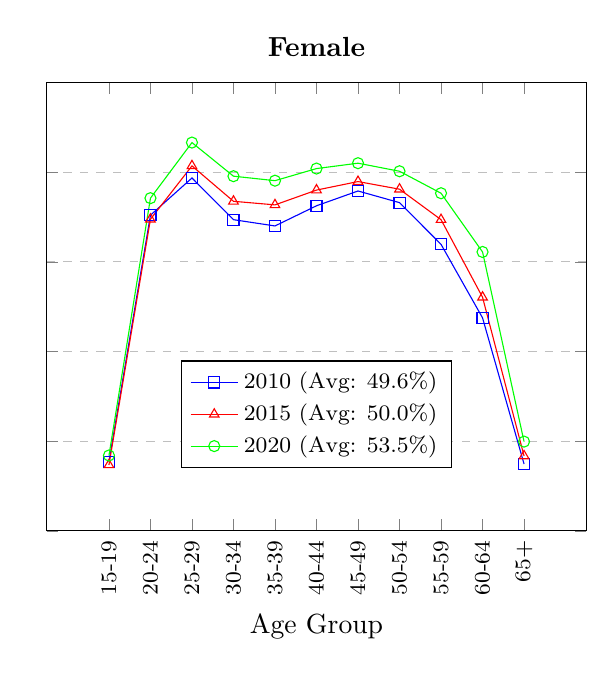
\begin{tikzpicture}
\begin{axis}[
    title={\textbf{Female}},
    xlabel={Age Group},
    ylabel={},
    xmin=0, xmax=12,
    ymin=0, ymax=100,
    xtick={1,2,3,4,5,6,7,8,9,10,11},
    xticklabels={15-19,20-24,25-29,30-34,35-39,40-44,45-49,50-54,55-59,60-64,65+},
    x tick label style={rotate=90,anchor=east,font=\footnotesize},
    legend style={at={(0.5,0.38)},anchor=north,font=\footnotesize,
                  cells={anchor=west},
                  legend columns=1,
                  draw=black,fill=white,align=left},
    ymajorgrids=true,
    grid style=dashed,
    yticklabels={,,},
    enlarge x limits={abs=0.5},
]

\addplot[color=blue,mark=square,] coordinates {
    (1,15.4)(2,70.4)(3,78.7)(4,69.4)(5,68.0)(6,72.5)(7,75.8)(8,73.2)(9,63.9)(10,47.5)(11,14.9)
};

\addplot[color=red,mark=triangle,] coordinates {
    (1,14.7)(2,69.5)(3,81.4)(4,73.5)(5,72.7)(6,76.0)(7,77.9)(8,76.2)(9,69.4)(10,52.1)(11,16.7)
};

\addplot[color=green,mark=o,] coordinates {
    (1,16.8)(2,74.2)(3,86.6)(4,79.1)(5,78.1)(6,80.8)(7,82.0)(8,80.2)(9,75.3)(10,62.2)(11,19.9)
};

\legend{
    2010 (Avg: 49.6\%),
    2015 (Avg: 50.0\%),
    2020 (Avg: 53.5\%)
}
\end{axis}
\end{tikzpicture}
\end{minipage}
\end{subfigure}

\vspace{0.5cm}

\begin{minipage}{\textwidth}
\footnotesize
\textit{Note} Labor force participation rates from the 2010, 2015, and 2020 Population Censuses. The ratio of the labor force to the population aged 15 and over (excluding those with "unknown" labor force status).

\end{minipage}

\caption{Labour Force Participation Rate by Age (Five-Year Groups) and Gender - Fukushima/Japan}

\label{fig:fukushima_labour_force_participation_rate}

\end{figure}

%%%%%%%%%%%%%%%%%%%%%%%%%%%%%%%%%%%%%%%%%%%%%
%%%%%%%%%%%%%%%%%%%%%%%%%%%%%%%%%%%%%%%%%%%%%%
% Hello work job openings
%%%%%%%%%%%%%%%%%%%%%%%%%%%%%%%%%%%%%%%%%%%%%%

\begin{figure}[h!]
    \centering
    \includegraphics[width=0.9\textwidth]{New Job Openings.jpeg}  % 幅を本文の80%に設定
    \caption{Hello Work Job Openings and Applicants in Fukushima}
    \label{fig:new_job_openings}
\end{figure}


%Although the number of job openings in the three disaster-affected prefectures of Iwate, Miyagi, and Fukushima initially decreased significantly immediately after the disaster, they have since outperformed the national average. This improvement is largely attributed to the reconstruction demand, including a surge in the construction industry. The first research question of this study investigates how the gender employment gap has evolved under such circumstances.
%%%%%%%%%%%%%%%%%%%%%%%%%%%%%%%%%%%%%%%%%%%%%%


%%%%%%%%%%%%%%%%%%%%%%%%%%%%%%%%%%%%%%%%%%%%%%
%Women ratio on the number of applicants in Fukushima
%%%%%%%%%%%%%%%%%%%%%%%%%%%%%%%%%%%%%%%%%%%%%%
\begin{figure}[h!]
    \centering
    \includegraphics[width=0.9\textwidth]{Women ratio on the number of job applicants.jpg}  % 幅を本文の80%に設定
    \caption{Women Ratio on the Number of Applicants in Fukushima}
    \label{fig:fukushima_Women_ratio_on_applicant}
\end{figure}
%%%%%%%%%%%%%%%%%%%%%%%%%%%%%%%%%%%%%%%%%%%%%%

%%%%%%%%%%%%%%%%%%%%%%%%%%%%%%%%%%%%%%%%%%%%%%
%Women ratio on the number of active job seekers
%%%%%%%%%%%%%%%%%%%%%%%%%%%%%%%%%%%%%%%%%%%%%%

\begin{figure}[h!]
    \centering
    \includegraphics[width=0.9\textwidth]{Women ratio on the number of active job seekers2.jpeg}  % 幅を本文の80%に設定
    \caption{Women ratio on the Number of Active Job Seekers in Fukushima}
    \label{fig:women_ratio_fukushima}
\end{figure}


%%%%%%%%%%%%%%%%%%%%%%%%%%%%%%%%%%%%%%%%%%%%%%
%Number of Unemployment Insurance Decisions
%%%%%%%%%%%%%%%%%%%%%%%%%%%%%%%%%%%%%%%%%%%%%%

\begin{figure}[h!]
    \centering
    \includegraphics[width=0.9\textwidth]{Number of Unemployment Insurance decisions.jpg}  % 幅を本文の80%に設定
    \caption{Number of Unemployment Insurance Decisions by Gender in Fukushima}
    \label{fig:employment_insurance_decisions}
\end{figure}

%%%%%%%%%%%%%%%%%%%%%%%%%%%%%%%%%%%%%%%%%%%%%%

%%%%%%%%%%%%%%%%%%%%%%%%%%%%%%%%%%%%%%%%%%%%%%
%Women ratio on the number of Unemployment Insurance Recipients
%%%%%%%%%%%%%%%%%%%%%%%%%%%%%%%%%%%%%%%%%%%%%%

\begin{figure}[h!]
    \centering
    \includegraphics[width=0.9\textwidth]{Number of Actual Unemployment Insurance Recipients2.jpeg}  % 幅を本文の80%に設定
    \caption{Women Ratio on the Number of Unemployment Insurance Recipients in Fukushima}
    \label{fig:women_ratio_fukushima2}
\end{figure}

%%%%%%%%%%%%%%%%%%%%%%%%%%%%%%%%%%%%%%%%%%%%%%




%%%%%%%%%%%%%%%%%%%%%%%%%%%%%%%%%%%%%%%%%%%%%%
% JGSS analysis
%%%%%%%%%%%%%%%%%%%%%%%%%%%%%%%%%%%%%%%%%%%%%%%%%%

\begin{figure}[ht!]
    \centering
    % Subfigure for the Kernel Density Graph
    \begin{subfigure}[t]{\textwidth}
        \centering
        \includegraphics[width=0.9\textwidth]{Kernel density graphs of respondent’s annual income from main job.png}
        \caption{Kernel Density Graphs of Respondents' Annual Income from Main Job (Income Bands, $N=20,\!119$)}
        \label{fig:Kernel_density}
    \end{subfigure}
    
    \vspace{1em} % Adds vertical space between the graph and the table

    % Subfigure for the Mean Annual Income Table
    \begin{subfigure}[t]{\textwidth}
        \centering
        \scriptsize
        \setlength{\tabcolsep}{6pt} % Adjust column separation as needed
        \renewcommand{\arraystretch}{1.2} % Increase row height for better readability
        \begin{tabular}{llcccc}
            \toprule
            \multirow{2}{*}{\textbf{Gender}} & \multirow{2}{*}{\textbf{Prefecture}} & \multicolumn{2}{c}{\textbf{Mean Income}} & \multirow{2}{*}{\textbf{Change (\%)}} & \multirow{2}{*}{\textbf{P-value}} \\
            \cmidrule(lr){3-4}
            & & \textbf{Pre} & \textbf{Post} & & \\
            \midrule
            \multirow{2}{*}{Male} 
                & Affected & 7.967 & 7.835 & -1.67 & 0.654 \\
                & Unaffected & 8.660 & 8.300 & \ \quad -4.16*** & 0.000 \\
            \midrule
            \multirow{2}{*}{Female} 
                & Affected & 4.721 & 5.183 & \ +9.79* & 0.065 \\
                & Unaffected & 4.995 & 5.087 & +1.83 & 0.143 \\
            \bottomrule
            \multicolumn{6}{l}{\footnotesize $^{*} p<0.1$, $^{**} p<0.05$, $^{***} p<0.01$}
        \end{tabular}
        \caption{Mean Annual Income from Main Job: Pre/Post-Disaster Period (Income Bands, $N=20,\!119$)}
        \label{table:mean_of_annual_income}
    \end{subfigure}
    
    % Main Caption for the Combined Figure and Table
    \caption{Analysis of Respondents' Annual Income from Main Job and Mean Income Changes by Gender and Prefecture}
    \label{fig:combined_figure_table}
\end{figure}

%%%%%%%%%%%%%%%%%%%%%%%%%%%%%%%%%%%%%%%%%%%%%%%%%%%%%%%%%%%%

%%%%%%%%%%%%%%%%%%%%%%%%%%%%%%%%%%%%%%%%%%%%%%
% DID analysis
%%%%%%%%%%%%%%%%%%%%%%%%%%%%%%%%%%%%%%%%%%%%%%%%%%

%%%%%%%%%%%%%%%%%%%%%%%%%%%%%%%%%%%%%%%%%%%%%%%%%%%%
% Placebo_Employment Status%

\begin{table}[htbp]
\centering
\caption{Placebo Test: DID Estimates of Disaster Impact on Employment Status (2000-2005)}

\vspace{-0.2cm}
\resizebox{\linewidth}{!}{%
\begin{tabular}{@{}l*{6}{c}@{}}
          &\multicolumn{3}{c}{Male}                                &\multicolumn{3}{c}{Female}                              \\\cmidrule(lr){2-4}\cmidrule(lr){5-7}
          &\multicolumn{1}{c}{(1)}         &\multicolumn{1}{c}{(2)}         &\multicolumn{1}{c}{(3)}         &\multicolumn{1}{c}{(4)}         &\multicolumn{1}{c}{(5)}         &\multicolumn{1}{c}{(6)}         \\
\toprule
Placebo Disaster Impact (DID)&   -0.014\sym{***}&   -0.011\sym{***}&   -0.013\sym{***}&    0.001         &   -0.004\sym{**} &   -0.004\sym{**} \\
          &  (0.002)         &  (0.002)         &  (0.002)         &  (0.002)         &  (0.002)         &  (0.002)         \\
\addlinespace
Placebo Post-Period&   -0.033\sym{***}&   -0.016\sym{***}&   -0.014\sym{***}&   -0.009\sym{***}&    0.007\sym{***}&    0.006\sym{***}\\
          &  (0.002)         &  (0.002)         &  (0.002)         &  (0.002)         &  (0.002)         &  (0.002)         \\
\addlinespace
Married   &                  &    0.191\sym{***}&    0.118\sym{***}&                  &   -0.098\sym{***}&   -0.062\sym{***}\\
          &                  &  (0.006)         &  (0.004)         &                  &  (0.007)         &  (0.005)         \\
\midrule
Age       &       No         &      Yes         &      Yes         &       No         &      Yes         &      Yes         \\
Relationship with Head&       No         &       No         &      Yes         &       No         &       No         &      Yes         \\
Residence Type&       No         &       No         &      Yes         &       No         &       No         &      Yes         \\
Household Size&       No         &       No         &      Yes         &       No         &       No         &      Yes         \\
$\textit{N}$&   550771         &   550771         &   550771         &   606094         &   606094         &   606094         \\
$\textit{R}^2$&    0.005         &    0.397         &    0.415         &    0.003         &    0.257         &    0.270         \\
Control Mean&    0.707         &    0.707         &    0.707         &    0.471         &    0.471         &    0.471         \\
\bottomrule
\end{tabular}}
\\\multicolumn{7}{@{}p{\linewidth}}{\footnotesize Standard errors clustered at prefecture level in parentheses}\\
\multicolumn{7}{@{}p{\linewidth}}{\footnotesize $*p<0.1$, $**p<0.05$, $***p<0.01$}\\
\multicolumn{7}{@{}p{\linewidth}}{\footnotesize \textit{Note}: This table presents OLS estimates of the placebo disaster impact on employment status for both males and females using 2000 and 2005 population census data. Residence Duration is not included as it is unavailable in the 2005 data set. All models include prefecture fixed effects, and the error term is clustered at the prefecture level. The binary variable for marital status assigns 1 to those with a spouse present and 0 to those never married, widowed, or divorced. Control Mean represents the mean employment rate for the control group (non-Fukushima prefectures) in the pre-period (2000).}
\label{table:DID_Employment_Status_Placebo}

\end{table}
%%%%%%%%%%%%%%%%%%%%%%%%%%%%%%%%%%%%%%%%%%%%%%%%%%%%


% ----------------------------------------------------
% Placebo: DID analysis on Regular worker
% ----------------------------------------------------

\begin{table}[htbp]
\centering
\caption{Placebo Test: DID Estimates of Disaster Impact on Regular Worker Status (2000-2005)}

\vspace{-0.2cm}

\resizebox{\linewidth}{!}{%
\begin{tabular}{@{}l*{6}{c}@{}}
          &\multicolumn{3}{c}{Male}                                &\multicolumn{3}{c}{Female}                              \\\cmidrule(lr){2-4}\cmidrule(lr){5-7}
          &\multicolumn{1}{c}{(1)}         &\multicolumn{1}{c}{(2)}         &\multicolumn{1}{c}{(3)}         &\multicolumn{1}{c}{(4)}         &\multicolumn{1}{c}{(5)}         &\multicolumn{1}{c}{(6)}         \\
\toprule
Placebo Disaster Impact (DID)&   -0.009\sym{***}&   -0.007\sym{***}&   -0.009\sym{***}&   -0.005\sym{***}&   -0.009\sym{***}&   -0.009\sym{***}\\
          &  (0.002)         &  (0.002)         &  (0.002)         &  (0.001)         &  (0.001)         &  (0.001)         \\
\addlinespace
Placebo Post-Period&   -0.040\sym{***}&   -0.023\sym{***}&   -0.021\sym{***}&   -0.009\sym{***}&    0.003\sym{**} &    0.000         \\
          &  (0.002)         &  (0.002)         &  (0.002)         &  (0.001)         &  (0.001)         &  (0.001)         \\
\addlinespace
Married   &                  &    0.224\sym{***}&    0.130\sym{***}&                  &   -0.168\sym{***}&   -0.092\sym{***}\\
          &                  &  (0.006)         &  (0.004)         &                  &  (0.006)         &  (0.005)         \\
\midrule
Age Group &       No         &      Yes         &      Yes         &       No         &      Yes         &      Yes         \\
Relationship with Head&       No         &       No         &      Yes         &       No         &       No         &      Yes         \\
Residence Type&       No         &       No         &      Yes         &       No         &       No         &      Yes         \\
Household Size&       No         &       No         &      Yes         &       No         &       No         &      Yes         \\
$\textit{N}$&   550771         &   550771         &   550771         &   606094         &   606094         &   606094         \\
$\textit{R}^2$&    0.006         &    0.383         &    0.400         &    0.003         &    0.214         &    0.224         \\
Control Mean&    0.651         &    0.651         &    0.651         &    0.332         &    0.332         &    0.332         \\
\bottomrule
\end{tabular}}
\\\multicolumn{7}{@{}p{\linewidth}}{\footnotesize Standard errors clustered at prefecture level in parentheses}\\
\multicolumn{7}{@{}p{\linewidth}}{\footnotesize $*p<0.1$, $**p<0.05$, $***p<0.01$}\\
\multicolumn{7}{@{}p{\linewidth}}{\footnotesize \textit{Note}: This table presents OLS estimates of the placebo disaster impact on regular worker status for both males and females using 2000 and 2005 population census data, excluding metropolitan areas. Residence Duration is not included as it is unavailable in the 2005 data set. The occupation variable is also excluded. All models include prefecture fixed effects, and the error term is clustered at the prefecture level. Control Mean represents the average proportion of regular workers in non-Fukushima prefectures before the placebo disaster period.}

\label{tab:placebo_Regular_Worker}

\end{table}

% ----------------------------------------------------

%-------------------------------
%Placebo DID impact on Non-Regular worker status
%-------------------------------

\begin{table}[htbp]
\centering
\caption{Placebo Test: DID Estimates of Disaster Impact on Non-Regular Worker Status (2000-2005)}

\vspace{-0.2cm}

\resizebox{\linewidth}{!}{%
\begin{tabular}{@{}l*{6}{c}@{}}
          &\multicolumn{3}{c}{Male}                                &\multicolumn{3}{c}{Female}                              \\\cmidrule(lr){2-4}\cmidrule(lr){5-7}
          &\multicolumn{1}{c}{(1)}         &\multicolumn{1}{c}{(2)}         &\multicolumn{1}{c}{(3)}         &\multicolumn{1}{c}{(4)}         &\multicolumn{1}{c}{(5)}         &\multicolumn{1}{c}{(6)}         \\
\toprule
Placebo Disaster Impact (DID)&   -0.005\sym{***}&   -0.005\sym{***}&   -0.005\sym{***}&    0.005\sym{***}&    0.005\sym{***}&    0.006\sym{***}\\
          &  (0.001)         &  (0.001)         &  (0.001)         &  (0.001)         &  (0.001)         &  (0.001)         \\
\addlinespace
Placebo Post-Period&    0.007\sym{***}&    0.007\sym{***}&    0.007\sym{***}&    0.000         &    0.004\sym{***}&    0.006\sym{***}\\
          &  (0.001)         &  (0.001)         &  (0.001)         &  (0.001)         &  (0.001)         &  (0.001)         \\
\addlinespace
Married   &                  &   -0.033\sym{***}&   -0.037\sym{***}&                  &    0.070\sym{***}&    0.067\sym{***}\\
          &                  &  (0.001)         &  (0.001)         &                  &  (0.003)         &  (0.003)         \\
\midrule
Age Group &       No         &      Yes         &      Yes         &       No         &      Yes         &      Yes         \\
Residence Type&       No         &       No         &      Yes         &       No         &       No         &      Yes         \\
Relationship with Head&       No         &       No         &      Yes         &       No         &       No         &      Yes         \\
$\textit{N}$&   550771         &   550771         &   550771         &   606094         &   606094         &   606094         \\
$\textit{R}^2$&    0.001         &    0.021         &    0.024         &    0.002         &    0.038         &    0.042         \\
Control Mean&    0.056         &    0.056         &    0.056         &    0.139         &    0.139         &    0.139         \\
\bottomrule
\end{tabular}}
\\\multicolumn{7}{@{}p{\linewidth}}{\footnotesize Standard errors clustered at prefecture level in parentheses}\\
\multicolumn{7}{@{}p{\linewidth}}{\footnotesize $*p<0.1$, $**p<0.05$, $***p<0.01$}\\
\multicolumn{7}{@{}p{\linewidth}}{\footnotesize \textit{Note}: This table reports OLS estimates of the placebo disaster's impact on non-regular worker status for males and females using 2000 and 2005 census data, excluding metropolitan areas, with the sample restricted to the population aged 15 and above. The outcome variable includes individuals categorized as unknown. Occupation variables are excluded. All models include prefecture fixed effects, with standard errors clustered at the prefecture level. Control Mean represents the pre-placebo proportion of non-regular workers in non-Fukushima prefectures.}

\label{table:Placebo_DID_Non_Regular_Worker}

\end{table}

%-------------------------------

%-------------------------------
%Placebo DID impact on Each Employment Type
%-------------------------------
\begin{landscape}
\thispagestyle{fancy}
\fancyhf{}  % ヘッダーとフッターをクリア
\fancyhead[R]{\rotatebox[origin=c]{90}{\thepage}}  % ページ番号を90度回転して下部右に配置
\renewcommand{\headrulewidth}{0pt}  % ヘッダーラインを削除
\begin{table}[htbp]
\centering
\caption{Placebo DID Estimates of Disaster Impact on Different Employment Types by Gender}

\vspace{0.2cm}

\resizebox{\linewidth}{!}{%
\begin{tabular}{@{}l*{17}{c}@{}}
          &\multicolumn{2}{c}{Regular Employee} &\multicolumn{2}{c}{Executive}        &\multicolumn{2}{c}{Self-employed}    &\multicolumn{2}{c}{Dispatched Worker}&\multicolumn{2}{c}{Part-time Worker} &\multicolumn{2}{c}{Family Worker}    &\multicolumn{2}{c}{Unknown Worker}   \\\cmidrule(lr){2-3}\cmidrule(lr){4-5}\cmidrule(lr){6-7}\cmidrule(lr){8-9}\cmidrule(lr){10-11}\cmidrule(lr){12-13}\cmidrule(lr){14-15}
          &\multicolumn{1}{c}{(1)}&\multicolumn{1}{c}{(2)}&\multicolumn{1}{c}{(3)}&\multicolumn{1}{c}{(4)}&\multicolumn{1}{c}{(5)}&\multicolumn{1}{c}{(6)}&\multicolumn{1}{c}{(7)}&\multicolumn{1}{c}{(8)}&\multicolumn{1}{c}{(9)}&\multicolumn{1}{c}{(10)}&\multicolumn{1}{c}{(11)}&\multicolumn{1}{c}{(12)}&\multicolumn{1}{c}{(13)}&\multicolumn{1}{c}{(14)}\\
          &\multicolumn{1}{c}{Male}&\multicolumn{1}{c}{Female}&\multicolumn{1}{c}{Male}&\multicolumn{1}{c}{Female}&\multicolumn{1}{c}{Male}&\multicolumn{1}{c}{Female}&\multicolumn{1}{c}{Male}&\multicolumn{1}{c}{Female}&\multicolumn{1}{c}{Male}&\multicolumn{1}{c}{Female}&\multicolumn{1}{c}{Male}&\multicolumn{1}{c}{Female}&\multicolumn{1}{c}{Male}&\multicolumn{1}{c}{Female}\\
\toprule
Placebo Disaster Impact (DID)&   -0.014\sym{***}&   -0.008\sym{***}&    0.004\sym{***}&   -0.002\sym{***}&   -0.000         &    0.003\sym{***}&   -0.004\sym{***}&    0.003\sym{**} &    0.003\sym{***}&    0.000         &    0.000         &    0.000         &   -0.000\sym{***}&   -0.000\sym{***}\\
          &  (0.002)         &  (0.001)         &  (0.001)         &  (0.001)         &  (0.000)         &  (0.001)         &  (0.001)         &  (0.001)         &  (0.001)         &  (0.000)         &      (.)         &      (.)         &  (0.000)         &  (0.000)         \\
\addlinespace
Post-Placebo Period&   -0.012\sym{***}&    0.008\sym{***}&   -0.009\sym{***}&   -0.005\sym{***}&   -0.002\sym{***}&   -0.008\sym{***}&    0.009\sym{***}&    0.013\sym{***}&   -0.003\sym{***}&   -0.000         &    0.000         &    0.000         &    0.000         &    0.000         \\
          &  (0.002)         &  (0.001)         &  (0.001)         &  (0.001)         &  (0.000)         &  (0.001)         &  (0.001)         &  (0.001)         &  (0.001)         &  (0.000)         &      (.)         &      (.)         &  (0.000)         &  (0.000)         \\
\addlinespace
Married   &    0.147\sym{***}&   -0.145\sym{***}&    0.043\sym{***}&   -0.028\sym{***}&   -0.010\sym{***}&    0.066\sym{***}&   -0.023\sym{***}&    0.004\sym{***}&    0.034\sym{***}&    0.005\sym{***}&    0.000         &    0.000         &   -0.000         &    0.000         \\
          &  (0.006)         &  (0.006)         &  (0.002)         &  (0.001)         &  (0.001)         &  (0.003)         &  (0.001)         &  (0.001)         &  (0.001)         &  (0.000)         &      (.)         &      (.)         &  (0.000)         &  (0.000)         \\
\addlinespace
Age Group &      Yes         &      Yes         &      Yes         &      Yes         &      Yes         &      Yes         &      Yes         &      Yes         &      Yes         &      Yes         &      Yes         &      Yes         &      Yes         &      Yes         \\
\midrule
$\textit{N}$&  550,771         &  606,094         &  550,771         &  606,094         &  550,771         &  606,094         &  550,771         &  606,094         &  550,771         &  606,094         &  550,771         &  606,094         &  550,771         &  606,094         \\
$\textit{R}^2$&    0.349         &    0.223         &    0.062         &    0.016         &    0.006         &    0.041         &    0.025         &    0.030         &    0.024         &    0.008         &        .         &        .         &    0.000         &    0.000         \\
Control Mean&    0.488         &    0.285         &    0.117         &    0.033         &    0.015         &    0.061         &    0.041         &    0.079         &    0.046         &    0.014         &    0.000         &    0.000         &    0.000         &    0.000         \\
\bottomrule
\end{tabular}}
\raggedright
\\\\{\linewidth}{\tiny Standard errors clustered at prefecture level in parentheses}\\\\
\vspace{-0.2cm}
\\\\{\linewidth}{\tiny $*p<0.1$, $**p<0.05$, $***p<0.01$}\\\\
\\
\vspace{0.1cm}
  {\setlength{\baselineskip}{0.9\baselineskip}
  \parbox{\linewidth}{\tiny
  \textit{Note}: This table presents Placebo DID estimates of the impact of the disaster on different employment types by gender. The dependent variable for each model is a binary indicator for the respective employment type. All models include prefecture fixed effects and age group fixed effects. The error term is clustered at the prefecture level. The binary variable for marital status assigns 1 to those with a spouse present and 0 to those never married, widowed, or divorced. Metropolitan areas (Tokyo, Kanagawa, Saitama, Chiba, Osaka, Kyoto, Hyogo, and Aichi) are excluded from the analysis. Control Mean represents the mean of the dependent variable for the control group (non-Fukushima) in the pre-placebo period.}}
\end{table}

\label{table:Placebo_DID_Each_Employment_Type}

\end{landscape}

%-------------------------------


%%%%%%%%%%%%%%%%%%%%%%%%%%%%%%%%%%%%%%%%%










%%%%%%%%%%%%%%%%%%%%%%%%%%%%%%%%%%%%%%%%%%%%%%%%%%%%%%%%%%%%
\begin{table}[htbp]
\centering
\caption{Difference in the Number of Workers (2010 vs 2015) in Fukushima}
\scriptsize
\begin{tabular}{l *{9}{S[table-format=-5.0]}}
\toprule
\multirow{3}{*}{Occupation} & {\multirow{3}{*}{\makecell[c]{\textbf{Total}\\\underline{(Reg +}\\\underline{Non-reg)}}}} & \multicolumn{4}{c}{\textbf{Regular}} & \multicolumn{4}{c}{\textbf{Non-regular}} \\
\cmidrule(lr){3-6} \cmidrule(lr){7-10}
& & {\multirow{2}{*}{\makecell[c]{\underline{Regular}\\\underline{(Total)}}}} & {Regular} & {Exec.} & {Self-} & {\multirow{2}{*}{\makecell[c]{\underline{Non-reg.}\\\underline{(Total)}}}} & {Disp.} & {Part-time,} & {Family} \\
& & & {empl.} & & {empl.} & & {workers} & {temp.} & {workers} \\
\midrule
\multicolumn{10}{c}{\textbf{Male}} \\
\midrule
Total & 1289 & -545 & 10591 & -1055 & -10081 & 1834 & 870 & 2719 & -1755 \\
Admin. \& managerial & -84 & -28 & -898 & 1296 & -426 & -52 & 0 & -52 & 0 \\
Prof. \& technical & 3521 & 3186 & 3400 & -119 & -95 & 335 & 112 & 263 & -40 \\
Clerical & 9364 & 7612 & 7251 & 276 & 85 & 1752 & 828 & 925 & -1 \\
Sales & -9636 & -8513 & -5186 & -1813 & -1514 & -1123 & -29 & -692 & -402 \\
Service & -1069 & -441 & 395 & -141 & -695 & -628 & 67 & -596 & -99 \\
Security & 1184 & 1094 & 1142 & -1 & -47 & 90 & 0 & 90 & 0 \\
Agri., forest. \& fish. & -6669 & -5959 & -383 & 32 & -5608 & -710 & -16 & -6 & -688 \\
Manufacturing & -14864 & -12017 & -10002 & -614 & -1401 & -2847 & -1668 & -768 & -411 \\
Trans. \& machine op. & 1042 & 596 & 747 & 19 & -170 & 446 & 122 & 308 & 16 \\
Constr. \& mining & 13740 & 11435 & 11403 & 85 & -53 & 2319 & 0 & 2211 & 108 \\
Carrying, clean., pack. & 7279 & 4519 & 4291 & -67 & 295 & 2760 & 1657 & 1179 & -76 \\
Not Classifiable & -2569 & -2049 & -1569 & 2 & -482 & -520 & -209 & -153 & -158 \\
\midrule
\multicolumn{10}{c}{\textbf{Female}} \\
\midrule
Total & -14626 & -1518 & 208 & 24 & -1750 & -13108 & -194 & -5413 & -7501 \\
Admin. \& managerial & 141 & 173 & -131 & 337 & -33 & -14 & 0 & -14 & 0 \\
Prof. \& technical & 2629 & 1957 & 2245 & 48 & -336 & 672 & -114 & 872 & -86 \\
Clerical & 4734 & 2516 & 2034 & 384 & 98 & 2218 & 921 & 1541 & -244 \\
Sales & -6188 & -2072 & -1053 & -489 & -530 & -4116 & -184 & -2580 & -1352 \\
Service & -2922 & 284 & 1496 & -140 & -1072 & -3206 & 27 & -2359 & -874 \\
Security & -33 & 87 & 72 & 8 & 7 & -120 & 0 & -120 & 0 \\
Agri., forest. \& fish. & -3950 & -127 & 10 & -17 & -120 & -3823 & -16 & -53 & -3754 \\
Manufacturing & -8632 & -4003 & -3494 & -73 & -436 & -4629 & -765 & -3236 & -628 \\
Trans. \& machine op. & 103 & 78 & 29 & -7 & 56 & 25 & -20 & 59 & -14 \\
Constr. \& mining & 328 & 96 & 124 & -27 & -1 & 222 & 0 & 208 & 14 \\
Carrying, clean., pack. & 646 & 12 & -329 & 33 & 308 & 634 & 26 & 537 & 71 \\
Not Classifiable & -1502 & -519 & -795 & -33 & 309 & -983 & -89 & -278 & -616 \\
\bottomrule
\end{tabular}

\addlinespace[0.35em]

\raggedright
\scriptsize
\textit{Note}: This table presents changes in the number of workers aged 15 years and over in Fukushima Prefecture between 2010 and 2015. The data is reorganized from the original census categories, which include regular employees, dispatched workers, part-time workers, executives, self-employed (with and without employees), family workers, and home-based workers. Workers with unclassifiable employment status are excluded from this analysis.\\
\textit{Source}: 2010 and 2015 Population Census.\\
\label{table:difference_workers_fukushima}
\end{table}
%%%%%%%%%%%%%%%%%%%%%%%%%%%%%%%%%%%%%%%%%%%%%%%%%%%%%%%%%%%%

%%%%%%%%%%%%%%%%%%%%%%%%%%
%Employment categories

\begin{table}[htbp]
\centering
\caption{Employment Types Used in Population Census and Study Classification}
\small
\begin{tabular}{>{\raggedright\arraybackslash}p{0.3\textwidth}>{\raggedright\arraybackslash}p{0.4\textwidth}>{\raggedright\arraybackslash}p{0.2\textwidth}}
\toprule
\textbf{Census Category} & \textbf{Definition} & \textbf{Study Classification} \\
\midrule
Regular employees & Regular employee has an indefinite employment contract with the employer. & \multirow{3}{*}{Regular workers} \\
\cmidrule{1-2}
Executives & Directors of a company or a corporation including managing directors. & \\
\cmidrule{1-2}
Self-employed & Persons who ran a business with or without employees. & \\
\midrule
Dispatched workers from temporary labour agency & Dispatched worker from temporary labour agency based on relevant low. & \multirow{3}{*}{Non-regular workers} \\
\cmidrule{1-2}
Part-time/temporary employees and others & "Part-time worker", "Arbeit (temporary worker)" and "Contract employee or entrusted employee". & \\
\cmidrule{1-2}
Family workers & Persons who worked in a business operated by a member of the household in which they lived. & \\
\bottomrule
\end{tabular}
\label{tab:employment_status}
\begin{flushleft}
\footnotesize
\textit{Note}: This table shows the employment type categories used in the Population Census and how I classified in this study. "Self-employed" combines both categories of self-employed (with and without employees) from the census. "Persons doing home handicraft" from the census are included in the "Family workers" category.\\
\textit{Source}: Adapted from Statistics Bureau of Japan, Population Census webpage: \url{https://www.stat.go.jp/english/data/kokusei/index.html}
\end{flushleft}

\label{table:employment_category}

\end{table}

%%%%%%%%%%%%%%%%%%%%%%%%%%



%%%%%%%%%%%%%%%%%%%%%%%%%%%%%%%%%


%%%%%%%%%%%%%%%%%%%%%%%%%%%%%%%%%

\begin{figure}[htbp]

\centering

% 2010 Figure

\begin{subfigure}{\textwidth}
\centering
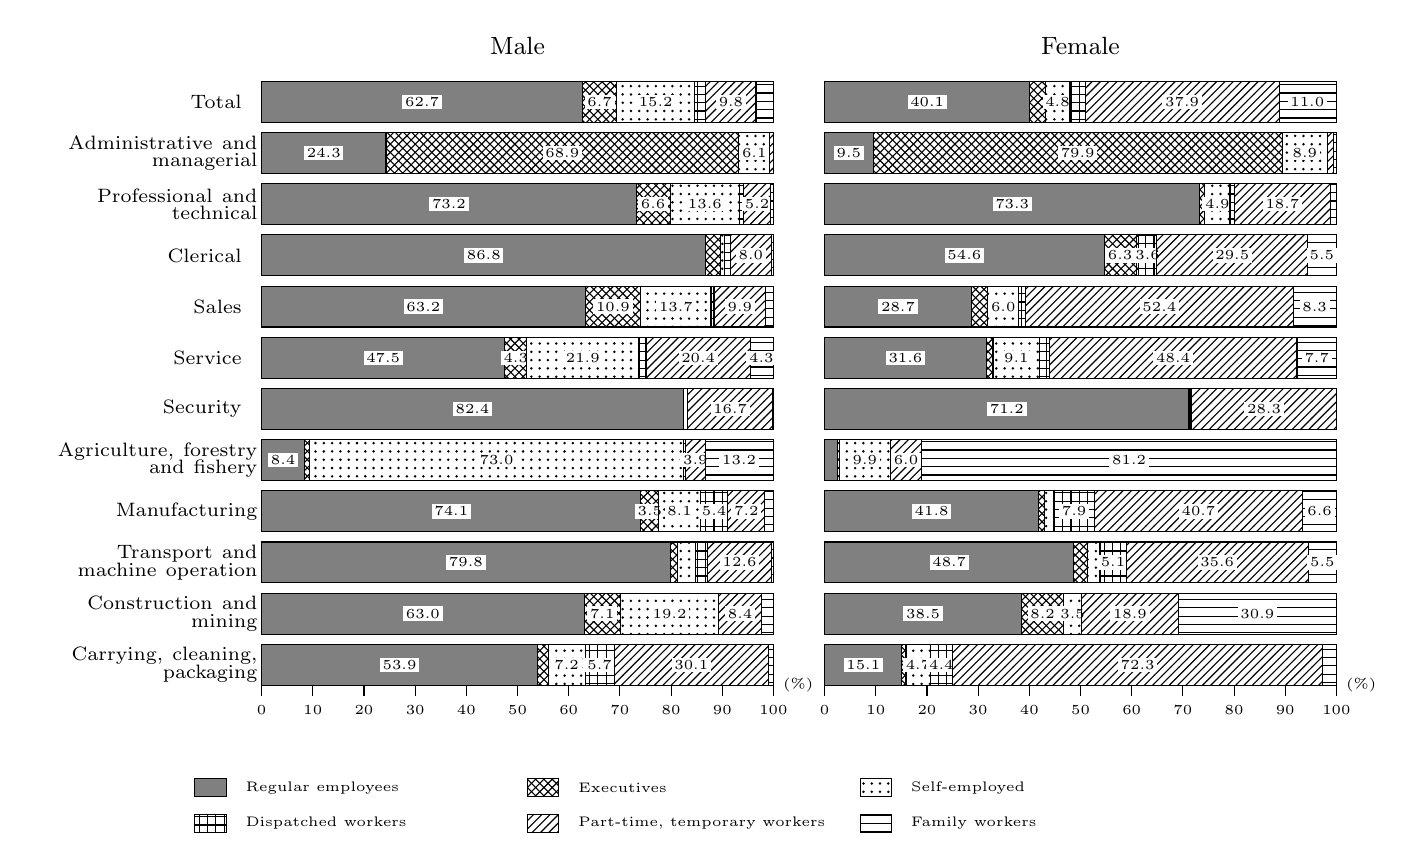
\begin{tikzpicture}[scale=0.65,xshift=-2cm]

\definecolor{color1}{RGB}{128,128,128}
\definecolor{color2}{RGB}{200,200,200}
\definecolor{color3}{RGB}{220,220,220}
\definecolor{color4}{RGB}{180,180,180}
\definecolor{color5}{RGB}{100,100,100}
\definecolor{color6}{RGB}{60,60,60}

% Function to draw a stacked bar
\newcommand{\stackedbar}[8]{
    \draw[fill=color1] (#1,#2) rectangle (#1+#3/10,#2+0.8);
    \pgfmathsetmacro{\result}{(#3 >= 3.5) ? 1 : 0}
    \ifnum\result>0
        \node[font=\tiny,fill=white,text=black,inner sep=1pt] at (#1+#3/20,#2+0.4) {#3};
    \fi
    \draw[fill=color2, pattern=crosshatch] (#1+#3/10,#2) rectangle (#1+#3/10+#4/10,#2+0.8);
    \pgfmathsetmacro{\result}{(#4 >= 3.5) ? 1 : 0}
    \ifnum\result>0
        \node[font=\tiny,fill=white,text=black,inner sep=1pt] at (#1+#3/10+#4/20,#2+0.4) {#4};
    \fi
    \draw[fill=color3, pattern=dots] (#1+#3/10+#4/10,#2) rectangle (#1+#3/10+#4/10+#5/10,#2+0.8);
    \pgfmathsetmacro{\result}{(#5 >= 3.5) ? 1 : 0}
    \ifnum\result>0
        \node[font=\tiny,fill=white,text=black,inner sep=1pt] at (#1+#3/10+#4/10+#5/20,#2+0.4) {#5};
    \fi
    \draw[fill=color4, pattern=grid] (#1+#3/10+#4/10+#5/10,#2) rectangle (#1+#3/10+#4/10+#5/10+#6/10,#2+0.8);
    \pgfmathsetmacro{\result}{(#6 >= 3.5) ? 1 : 0}
    \ifnum\result>0
        \node[font=\tiny,fill=white,text=black,inner sep=1pt] at (#1+#3/10+#4/10+#5/10+#6/20,#2+0.4) {#6};
    \fi
    \draw[fill=color5, pattern=north east lines] (#1+#3/10+#4/10+#5/10+#6/10,#2) rectangle (#1+#3/10+#4/10+#5/10+#6/10+#7/10,#2+0.8);
    \pgfmathsetmacro{\result}{(#7 >= 3.5) ? 1 : 0}
    \ifnum\result>0
        \node[font=\tiny,fill=white,text=black,inner sep=1pt] at (#1+#3/10+#4/10+#5/10+#6/10+#7/20,#2+0.4) {#7};
    \fi
    \draw[fill=color6, pattern=horizontal lines] (#1+#3/10+#4/10+#5/10+#6/10+#7/10,#2) rectangle (#1+10,#2+0.8);
    \pgfmathsetmacro{\result}{(#8 >= 3.5) ? 1 : 0}
    \ifnum\result>0
        \node[font=\tiny,fill=white,text=black,inner sep=1pt] at (#1+#3/10+#4/10+#5/10+#6/10+#7/10+#8/20,#2+0.4) {#8};
    \fi
}

% Male bars
\begin{scope}[xshift=-5.5cm]
\stackedbar{0}{11}{62.7}{6.7}{15.2}{2.2}{9.8}{2.3}
\node[anchor=east, text width=2.6cm, align=right] at (-0.2,11.4) {\scriptsize Total};
\stackedbar{0}{10}{24.3}{68.9}{6.1}{0}{0.7}{0}
\node[anchor=east, text width=2.6cm, align=right] at (-0.2,10.4) {\scriptsize\parbox[t]{2.8cm}{\setstretch{0.8}\raggedleft Administrative and managerial}};
\stackedbar{0}{9}{73.2}{6.6}{13.6}{0.8}{5.2}{0.6}
\node[anchor=east, text width=2.6cm, align=right] at (-0.2,9.4) {\scriptsize\parbox[t]{2.8cm}{\setstretch{0.8}\raggedleft Professional and technical}};
\stackedbar{0}{8}{86.8}{2.9}{0.7}{1.2}{8.0}{0.3}
\node[anchor=east, text width=2.6cm, align=right] at (-0.2,8.4) {\scriptsize Clerical};
\stackedbar{0}{7}{63.2}{10.9}{13.7}{0.7}{9.9}{1.6}
\node[anchor=east, text width=2.6cm, align=right] at (-0.2,7.4) {\scriptsize Sales};
\stackedbar{0}{6}{47.5}{4.3}{21.9}{1.4}{20.4}{4.3}
\node[anchor=east, text width=2.6cm, align=right] at (-0.2,6.4) {\scriptsize Service};
\stackedbar{0}{5}{82.4}{0.1}{0.7}{0}{16.7}{0}
\node[anchor=east, text width=2.6cm, align=right] at (-0.2,5.4) {\scriptsize Security};
\stackedbar{0}{4}{8.4}{1.0}{73.0}{0.4}{3.9}{13.2}
\node[anchor=east, text width=2.6cm, align=right] at (-0.2,4.4) {\scriptsize\parbox[t]{2.8cm}{\setstretch{0.8}\raggedleft Agriculture, forestry and fishery}};
\stackedbar{0}{3}{74.1}{3.5}{8.1}{5.4}{7.2}{1.5}
\node[anchor=east, text width=2.6cm, align=right] at (-0.2,3.4) {\scriptsize\parbox[t]{2.8cm}{\setstretch{0.8}\raggedleft Manufacturing}};
\stackedbar{0}{2}{79.8}{1.5}{3.4}{2.4}{12.6}{0.2}
\node[anchor=east, text width=2.6cm, align=right] at (-0.2,2.4) {\scriptsize\parbox[t]{2.8cm}{\setstretch{0.8}\raggedleft Transport and machine operation}};
\stackedbar{0}{1}{63.0}{7.1}{19.2}{0}{8.4}{2.2}
\node[anchor=east, text width=2.6cm, align=right] at (-0.2,1.4) {\scriptsize\parbox[t]{2.8cm}{\setstretch{0.8}\raggedleft Construction and mining}};
\stackedbar{0}{0}{53.9}{2.1}{7.2}{5.7}{30.1}{1.0}
\node[anchor=east, text width=2.6cm, align=right] at (-0.2,0.4) {\scriptsize\parbox[t]{2.8cm}{\setstretch{0.8}\raggedleft Carrying, cleaning, packaging}};

% X-axis for Male
\draw (0,0) -- (10,0);
\foreach \x in {0,1,...,10}
    \draw (\x,0) -- (\x,-0.2) node[anchor=north] {\tiny \ifnum\x=0 0\else\x0\fi};
\node[anchor=west] at (10,0) {\tiny (\%)};

% Label for Male
\node[anchor=center] at (5,12.5) {\small Male};
\end{scope}

% Female bars
\begin{scope}[xshift=5.5cm]
\stackedbar{0}{11}{40.1}{3.0}{4.8}{3.0}{37.9}{11.0}
\stackedbar{0}{10}{9.5}{79.9}{8.9}{0}{1.1}{0.6}
\stackedbar{0}{9}{73.3}{1.0}{4.9}{0.9}{18.7}{1.2}
\stackedbar{0}{8}{54.6}{6.3}{0.4}{3.6}{29.5}{5.5}
\stackedbar{0}{7}{28.7}{3.2}{6.0}{1.3}{52.4}{8.3}
\stackedbar{0}{6}{31.6}{1.3}{9.1}{1.9}{48.4}{7.7}
\stackedbar{0}{5}{71.2}{0.2}{0.3}{0}{28.3}{0}
\stackedbar{0}{4}{2.5}{0.4}{9.9}{0.1}{6.0}{81.2}
\stackedbar{0}{3}{41.8}{1.1}{1.9}{7.9}{40.7}{6.6}
\stackedbar{0}{2}{48.7}{2.7}{2.4}{5.1}{35.6}{5.5}
\stackedbar{0}{1}{38.5}{8.2}{3.5}{0}{18.9}{30.9}
\stackedbar{0}{0}{15.1}{0.8}{4.7}{4.4}{72.3}{2.8}

% X-axis for Female
\draw (0,0) -- (10,0);
\foreach \x in {0,1,...,10}
    \draw (\x,0) -- (\x,-0.2) node[anchor=north] {\tiny \ifnum\x=0 0\else\x0\fi};
\node[anchor=west] at (10,0) {\tiny (\%)};

% Label for Female
\node[anchor=center] at (5,12.5) {\small Female};
\end{scope}

% Legend (2 rows, 3 columns)
\node[anchor=center, fill=color1, minimum width=0.4cm, minimum height=0.2cm, draw] at (-6.5,-2) {};
\node[anchor=west] at (-6,-2) {\tiny Regular employees};
\node[anchor=center, fill=color2, pattern=crosshatch, minimum width=0.4cm, minimum height=0.2cm, draw] at (0,-2) {};
\node[anchor=west] at (0.5,-2) {\tiny Executives};
\node[anchor=center, fill=color3, pattern=dots, minimum width=0.4cm, minimum height=0.2cm, draw] at (6.5,-2) {};
\node[anchor=west] at (7,-2) {\tiny Self-employed};
\node[anchor=center, fill=color4, pattern=grid, minimum width=0.4cm, minimum height=0.2cm, draw] at (-6.5,-2.7) {};
\node[anchor=west] at (-6,-2.7) {\tiny Dispatched workers};
\node[anchor=center, fill=color5, pattern=north east lines, minimum width=0.4cm, minimum height=0.2cm, draw] at (0,-2.7) {};
\node[anchor=west] at (0.5,-2.7) {\tiny Part-time, temporary workers};
\node[anchor=center, fill=color6, pattern=horizontal lines, minimum width=0.4cm, minimum height=0.2cm, draw] at (6.5,-2.7) {};
\node[anchor=west] at (7,-2.7) {\tiny Family workers};

\end{tikzpicture}
\caption{2010}
\label{fig:proportion_2010}
\end{subfigure}

%%%%%%%%%%%%%%%%%%%%%%%%%%%%%%%%%
\vspace{0.25cm} % 1cm分のスペースを空ける
%%%%%%%%%%%%%%%%%%%%%%%%%%%%%%%%%


% 2015 Figure

\begin{subfigure}{\textwidth}
\centering
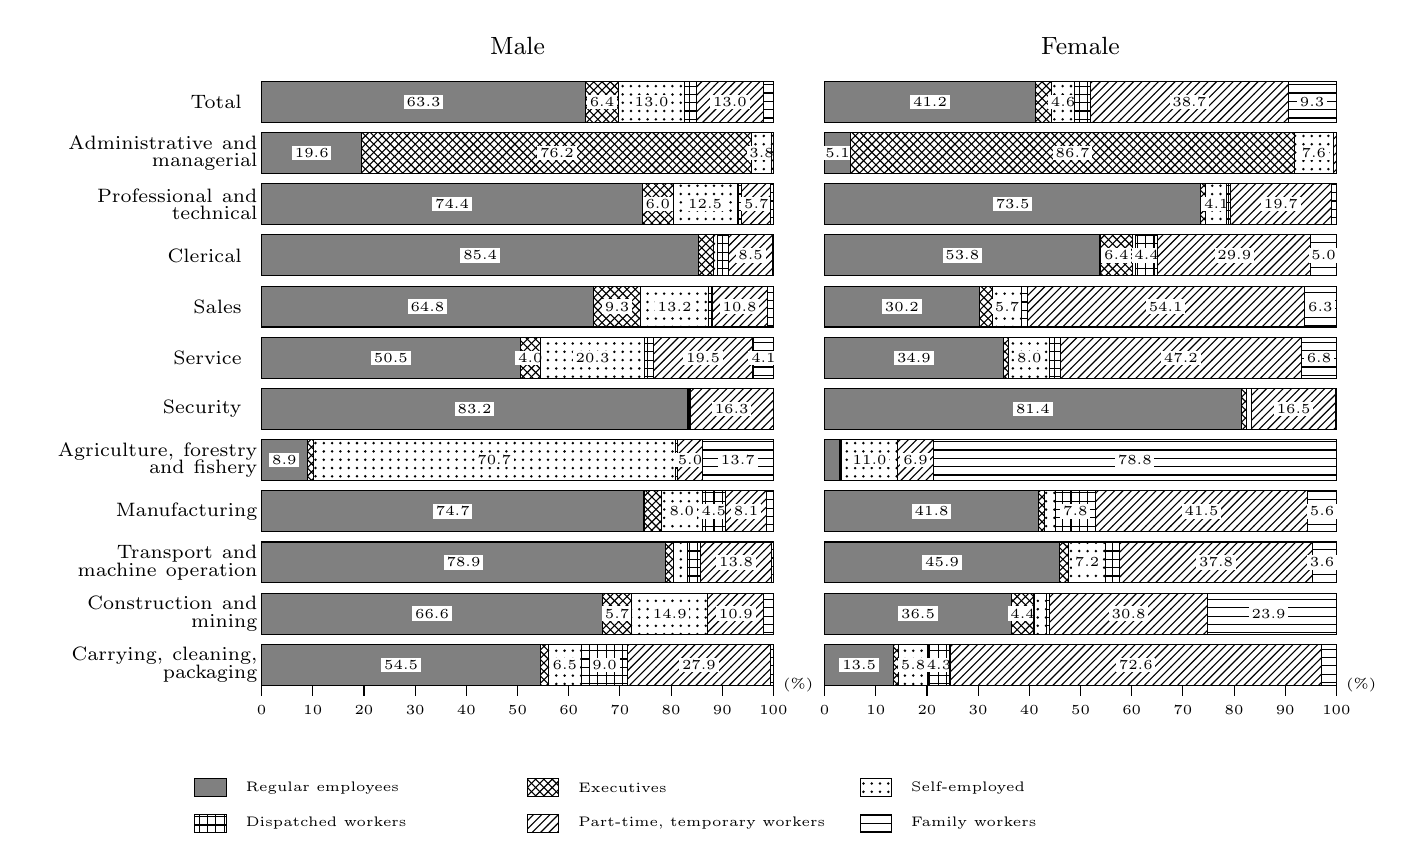
\begin{tikzpicture}
[scale=0.65,xshift=-2cm]
\definecolor{color1}{RGB}{128,128,128}
\definecolor{color2}{RGB}{200,200,200}
\definecolor{color3}{RGB}{220,220,220}
\definecolor{color4}{RGB}{180,180,180}
\definecolor{color5}{RGB}{100,100,100}
\definecolor{color6}{RGB}{60,60,60}

% Function to draw a stacked bar
\newcommand{\stackedbar}[8]{
    \draw[fill=color1] (#1,#2) rectangle (#1+#3/10,#2+0.8);
    \pgfmathsetmacro{\result}{(#3 >= 3.5) ? 1 : 0}
    \ifnum\result>0
        \node[font=\tiny,fill=white,text=black,inner sep=1pt] at (#1+#3/20,#2+0.4) {#3};
    \fi
    \draw[fill=color2, pattern=crosshatch] (#1+#3/10,#2) rectangle (#1+#3/10+#4/10,#2+0.8);
    \pgfmathsetmacro{\result}{(#4 >= 3.5) ? 1 : 0}
    \ifnum\result>0
        \node[font=\tiny,fill=white,text=black,inner sep=1pt] at (#1+#3/10+#4/20,#2+0.4) {#4};
    \fi
    \draw[fill=color3, pattern=dots] (#1+#3/10+#4/10,#2) rectangle (#1+#3/10+#4/10+#5/10,#2+0.8);
    \pgfmathsetmacro{\result}{(#5 >= 3.5) ? 1 : 0}
    \ifnum\result>0
        \node[font=\tiny,fill=white,text=black,inner sep=1pt] at (#1+#3/10+#4/10+#5/20,#2+0.4) {#5};
    \fi
    \draw[fill=color4, pattern=grid] (#1+#3/10+#4/10+#5/10,#2) rectangle (#1+#3/10+#4/10+#5/10+#6/10,#2+0.8);
    \pgfmathsetmacro{\result}{(#6 >= 3.5) ? 1 : 0}
    \ifnum\result>0
        \node[font=\tiny,fill=white,text=black,inner sep=1pt] at (#1+#3/10+#4/10+#5/10+#6/20,#2+0.4) {#6};
    \fi
    \draw[fill=color5, pattern=north east lines] (#1+#3/10+#4/10+#5/10+#6/10,#2) rectangle (#1+#3/10+#4/10+#5/10+#6/10+#7/10,#2+0.8);
    \pgfmathsetmacro{\result}{(#7 >= 3.5) ? 1 : 0}
    \ifnum\result>0
        \node[font=\tiny,fill=white,text=black,inner sep=1pt] at (#1+#3/10+#4/10+#5/10+#6/10+#7/20,#2+0.4) {#7};
    \fi
    \draw[fill=color6, pattern=horizontal lines] (#1+#3/10+#4/10+#5/10+#6/10+#7/10,#2) rectangle (#1+10,#2+0.8);
    \pgfmathsetmacro{\result}{(#8 >= 3.5) ? 1 : 0}
    \ifnum\result>0
        \node[font=\tiny,fill=white,text=black,inner sep=1pt] at (#1+#3/10+#4/10+#5/10+#6/10+#7/10+#8/20,#2+0.4) {#8};
    \fi
}

% Male bars
\begin{scope}[xshift=-5.5cm]
\stackedbar{0}{11}{63.3}{6.4}{13.0}{2.3}{13.0}{1.9}
\node[anchor=east, text width=2.6cm, align=right] at (-0.2,11.4) {\scriptsize Total};
\stackedbar{0}{10}{19.6}{76.2}{3.8}{0.0}{0.4}{0.0}
\node[anchor=east, text width=2.6cm, align=right] at (-0.2,10.4) {\scriptsize\parbox[t]{2.8cm}{\setstretch{0.8}\raggedleft Administrative and managerial}};
\stackedbar{0}{9}{74.4}{6.0}{12.5}{0.9}{5.7}{0.5}
\node[anchor=east, text width=2.6cm, align=right] at (-0.2,9.4) {\scriptsize\parbox[t]{2.8cm}{\setstretch{0.8}\raggedleft Professional and technical}};
\stackedbar{0}{8}{85.4}{2.9}{0.7}{2.3}{8.5}{0.3}
\node[anchor=east, text width=2.6cm, align=right] at (-0.2,8.4) {\scriptsize Clerical};
\stackedbar{0}{7}{64.8}{9.3}{13.2}{0.7}{10.8}{1.1}
\node[anchor=east, text width=2.6cm, align=right] at (-0.2,7.4) {\scriptsize Sales};
\stackedbar{0}{6}{50.5}{4.0}{20.3}{1.7}{19.5}{4.1}
\node[anchor=east, text width=2.6cm, align=right] at (-0.2,6.4) {\scriptsize Service};
\stackedbar{0}{5}{83.2}{0.1}{0.4}{0.0}{16.3}{0.0}
\node[anchor=east, text width=2.6cm, align=right] at (-0.2,5.4) {\scriptsize Security};
\stackedbar{0}{4}{8.9}{1.2}{70.7}{0.4}{5.0}{13.7}
\node[anchor=east, text width=2.6cm, align=right] at (-0.2,4.4) {\scriptsize\parbox[t]{2.8cm}{\setstretch{0.8}\raggedleft Agriculture, forestry and fishery}};
\stackedbar{0}{3}{74.7}{3.4}{8.0}{4.5}{8.1}{1.3}
\node[anchor=east, text width=2.6cm, align=right] at (-0.2,3.4) {\scriptsize\parbox[t]{2.8cm}{\setstretch{0.8}\raggedleft Manufacturing}};
\stackedbar{0}{2}{78.9}{1.5}{2.8}{2.6}{13.8}{0.3}
\node[anchor=east, text width=2.6cm, align=right] at (-0.2,2.4) {\scriptsize\parbox[t]{2.8cm}{\setstretch{0.8}\raggedleft Transport and machine operation}};
\stackedbar{0}{1}{66.6}{5.7}{14.9}{0.0}{10.9}{1.9}
\node[anchor=east, text width=2.6cm, align=right] at (-0.2,1.4) {\scriptsize\parbox[t]{2.8cm}{\setstretch{0.8}\raggedleft Construction and mining}};
\stackedbar{0}{0}{54.5}{1.5}{6.5}{9.0}{27.9}{0.6}
\node[anchor=east, text width=2.6cm, align=right] at (-0.2,0.4) {\scriptsize\parbox[t]{2.8cm}{\setstretch{0.8}\raggedleft Carrying, cleaning, packaging}};

% X-axis for Male
\draw (0,0) -- (10,0);
\foreach \x in {0,1,...,10}
    \draw (\x,0) -- (\x,-0.2) node[anchor=north] {\tiny \ifnum\x=0 0\else\x0\fi};
\node[anchor=west] at (10,0) {\tiny (\%)};

% Label for Male
\node[anchor=center] at (5,12.5) {\small Male};
\end{scope}

% Female bars
\begin{scope}[xshift=5.5cm]
\stackedbar{0}{11}{41.2}{3.1}{4.6}{3.0}{38.7}{9.3}
\stackedbar{0}{10}{5.1}{86.7}{7.6}{0.0}{0.6}{0.0}
\stackedbar{0}{9}{73.5}{1.0}{4.1}{0.7}{19.7}{1.0}
\stackedbar{0}{8}{53.8}{6.4}{0.5}{4.4}{29.9}{5.0}
\stackedbar{0}{7}{30.2}{2.6}{5.7}{1.1}{54.1}{6.3}
\stackedbar{0}{6}{34.9}{1.1}{8.0}{2.0}{47.2}{6.8}
\stackedbar{0}{5}{81.4}{1.0}{1.0}{0.0}{16.5}{0.0}
\stackedbar{0}{4}{3.0}{0.3}{11.0}{0.0}{6.9}{78.8}
\stackedbar{0}{3}{41.8}{1.1}{2.2}{7.8}{41.5}{5.6}
\stackedbar{0}{2}{45.9}{1.8}{7.2}{2.7}{37.8}{3.6}
\stackedbar{0}{1}{36.5}{4.4}{2.5}{0.6}{30.8}{23.9}
\stackedbar{0}{0}{13.5}{0.9}{5.8}{4.3}{72.6}{3.0}

% X-axis for Female
\draw (0,0) -- (10,0);
\foreach \x in {0,1,...,10}
    \draw (\x,0) -- (\x,-0.2) node[anchor=north] {\tiny \ifnum\x=0 0\else\x0\fi};
\node[anchor=west] at (10,0) {\tiny (\%)};

% Label for Female
\node[anchor=center] at (5,12.5) {\small Female};
\end{scope}

% Legend (2 rows, 3 columns)
\node[anchor=center, fill=color1, minimum width=0.4cm, minimum height=0.2cm, draw] at (-6.5,-2) {};
\node[anchor=west] at (-6,-2) {\tiny Regular employees};
\node[anchor=center, fill=color2, pattern=crosshatch, minimum width=0.4cm, minimum height=0.2cm, draw] at (0,-2) {};
\node[anchor=west] at (0.5,-2) {\tiny Executives};
\node[anchor=center, fill=color3, pattern=dots, minimum width=0.4cm, minimum height=0.2cm, draw] at (6.5,-2) {};
\node[anchor=west] at (7,-2) {\tiny Self-employed};
\node[anchor=center, fill=color4, pattern=grid, minimum width=0.4cm, minimum height=0.2cm, draw] at (-6.5,-2.7) {};
\node[anchor=west] at (-6,-2.7) {\tiny Dispatched workers};
\node[anchor=center, fill=color5, pattern=north east lines, minimum width=0.4cm, minimum height=0.2cm, draw] at (0,-2.7) {};
\node[anchor=west] at (0.5,-2.7) {\tiny Part-time, temporary workers};
\node[anchor=center, fill=color6, pattern=horizontal lines, minimum width=0.4cm, minimum height=0.2cm, draw] at (6.5,-2.7) {};
\node[anchor=west] at (7,-2.7) {\tiny Family workers};

\end{tikzpicture}
\caption{2015}
\label{fig:proportion_2015}
\end{subfigure}

\vspace{-0.40cm}

\begin{flushleft} {\footnotesize \textit{Note}: This graph represents employed individuals aged 15 and above in Fukushima Prefecture. Unclassifiable occupations are excluded from the analysis.}

{\footnotesize \textit{Source}: 2010 and 2015 Population Census.}

\caption{Proportion of Employed Persons Aged 15 and Over by Occupation, Employment Type, and Gender in Fukushima} \end{flushleft}

\label{fig_proportion_of_employed}

\end{figure}

%%%%%%%%%%%%%%%%%%%%%%%%%
\clearpage
% すべての文献を引用リストに追加
%\nocite{*}

% 参考文献リストの場所を示す
\bibliography{references}  % 'references.bib'ファイルの名前を指定
\bibliographystyle{plain}  % 引用スタイルを指定


\end{document}
